%% LyX 2.2.1 created this file.  For more info, see http://www.lyx.org/.
%% Do not edit unless you really know what you are doing.
\documentclass[11pt,czech,czech,pointednumbers,normalheadings,liststotoc,idxtotoc]{scrreprt}
\usepackage[utf8]{inputenc}
\usepackage[a4paper]{geometry}
\geometry{verbose,tmargin=2cm,bmargin=2cm,lmargin=3cm,rmargin=2.5cm,headheight=1cm,footskip=1cm}
\usepackage{fancyhdr}
\pagestyle{fancy}
\setlength{\parskip}{\smallskipamount}
\setlength{\parindent}{0pt}
\usepackage{pifont}
\usepackage{float}
\usepackage[czech]{babel}
\usepackage{graphicx}
\usepackage{setspace}
\usepackage{fancyref}
\usepackage[hyphens]{url}
\usepackage{hyperref}
\usepackage{enumitem}
\usepackage{babel}
\usepackage{todonotes}
\usepackage{verbatim}
\usepackage{forest}

\usepackage{datatool}% http://ctan.org/pkg/datatool
\newcommand{\sortitem}[1]{%
  \DTLnewrow{list}% Create a new entry
  \DTLnewdbentry{list}{description}{#1}% Add entry as description
}
\newenvironment{sortedlist}{%
  \DTLifdbexists{list}{\DTLcleardb{list}}{\DTLnewdb{list}}% Create new/discard old list
}{%
  \DTLsort{description}{list}% Sort list
  \begin{itemize}%
    \DTLforeach*{list}{\theDesc=description}{%
      \item \theDesc}% Print each item
  \end{itemize}%
}

\definecolor{folderbg}{RGB}{124,166,198}
\definecolor{folderborder}{RGB}{110,144,169}

\def\Size{4pt}
\tikzset{
  folder/.pic={
    \filldraw[draw=folderborder,top color=folderbg!50,bottom color=folderbg]
      (-1.05*\Size,0.2\Size+5pt) rectangle ++(.75*\Size,-0.2\Size-5pt);  
    \filldraw[draw=folderborder,top color=folderbg!50,bottom color=folderbg]
      (-1.15*\Size,-\Size) rectangle (1.15*\Size,\Size);
  }
}

\onehalfspacing

\makeatletter
%%%%%%%%%%%%%%%%%%%%%%%%%%%%%% Textclass specific LaTeX commands.
\usepackage{wasysym}

%%%%%%%%%%%%%%%%%%%%%%%%%%%%%% User specified LaTeX commands.
\usepackage{graphics}
\usepackage{hyperref}
\usepackage{ifthen}
\usepackage{soul}
\usepackage{colortbl}

\makeglossary
\renewcommand{\arraystretch}{1.25}

\widowpenalty = 10000 \relax
\clubpenalty = 10000 \relax

%********** nastaveni pro float objekty

\renewcommand{\textfraction}{0.15}
\renewcommand{\topfraction}{0.85}
\renewcommand{\bottomfraction}{0.65}
\renewcommand{\floatpagefraction}{0.60}

%********** nastaveni fancyhdr
\renewcommand{\chaptermark}[1]{\markboth{\thechapter.\ #1}{}}
\fancyhf{}
\fancyhead[CO]{\small \leftmark} 
%\fancyhead[LE]{Qt --- programov\'an\'{\i} v p\v r\'{\i}kladech}
\fancyfoot[CE,CO]{\bfseries \thepage}

\fancypagestyle{plain}{%
\fancyhf{}
\fancyfoot[CE,CO]{\bfseries\thepage}
\renewcommand{\headrulewidth}{0pt} 
\renewcommand{\footrulewidth}{0pt}}

%styl pro zahlavi pismennych oddilu
\def\indkap #1{\vspace{0.4em}{\Large \textbf{#1}}\nopagebreak\vspace{0.8em}}

\renewcommand{\headrulewidth}{0.4pt} 
\renewcommand{\footrulewidth}{0pt} 

\widowpenalty = 5000 \relax
\clubpenalty = 5000 \relax

\usepackage{listings}
\usepackage{color}

\definecolor{lightgray}{rgb}{0.95, 0.95, 0.95}
\definecolor{darkgray}{rgb}{0.4, 0.4, 0.4}
\definecolor{purple}{rgb}{0.65, 0.12, 0.82}
\definecolor{editorGray}{rgb}{0.95, 0.95, 0.95}
\definecolor{editorOcher}{rgb}{1, 0.5, 0} % #FF7F00 -> rgb(239, 169, 0)
\definecolor{editorGreen}{rgb}{0, 0.5, 0} % #007C00 -> rgb(0, 124, 0)
\usepackage{upquote}
\usepackage{listings}
% CSS
\lstdefinelanguage{CSS}{
  keywords={color,background-image:,margin,padding,font,weight,display,position,top,left,right,bottom,list,style,border,size,white,space,min,width, transition:, transform:, transition-property, transition-duration, transition-timing-function},	
  sensitive=true,
  morecomment=[l]{//},
  morecomment=[s]{/*}{*/},
  morestring=[b]',
  morestring=[b]",
  alsoletter={:},
  alsodigit={-}
}

% JavaScript
\lstdefinelanguage{JavaScript}{
  morekeywords={typeof, new, true, false, catch, function, return, null, catch, switch, var, if, in, while, do, else, case, break},
  morecomment=[s]{/*}{*/},
  morecomment=[l]//,
  morestring=[b]",
  morestring=[b]'
}

\lstdefinelanguage{HTML5}{
  language=html,
  sensitive=true,	
  alsoletter={<>=-},	
  morecomment=[s]{<!-}{-->},
  tag=[s],
  otherkeywords={
  % General
  >,
  % Standard tags
	<!DOCTYPE,
  </html, <html, <head, <title, </title, <style, </style, <link, </head, <meta, />,
	% body
	</body, <body,
	% Divs
	</div, <div, </div>, 
	% Paragraphs
	</p, <p, </p>,
	% scripts
	</script, <script,
  % More tags...
  <canvas, /canvas>, <svg, <rect, <animateTransform, </rect>, </svg>, <video, <source, <iframe, </iframe>, </video>, <image, </image>
  },
  ndkeywords={
  % General
  =,
  % HTML attributes
  charset=, src=, id=, width=, height=, style=, type=, rel=, href=,
  % SVG attributes
  fill=, attributeName=, begin=, dur=, from=, to=, poster=, controls=, x=, y=, repeatCount=, xlink:href=,
  % CSS properties
  margin:, padding:, background-image:, border:, top:, left:, position:, width:, height:,
	% CSS3 properties
  transform:, -moz-transform:, -webkit-transform:,
  animation:, -webkit-animation:,
  transition:,  transition-duration:, transition-property:, transition-timing-function:,
  }
}

\lstset{%
  % General design
  backgroundcolor=\color{editorGray},
  basicstyle={\small\ttfamily},   
  frame=l,
  % line-numbers
  xleftmargin={0.75cm},
  numbers=left,
  stepnumber=1,
  firstnumber=1,
  numberfirstline=true,	
  % Code design
  identifierstyle=\color{black},
  keywordstyle=\color{blue}\bfseries,
  ndkeywordstyle=\color{editorGreen}\bfseries,
  stringstyle=\color{editorOcher}\ttfamily,
  commentstyle=\color{darkgray}\ttfamily,
  % Code
  language=HTML5,
  alsolanguage=JavaScript,
  alsodigit={.:;},	
  tabsize=2,
  showtabs=false,
  showspaces=false,
  showstringspaces=false,
  extendedchars=true,
  breaklines=true,
  captionpos=b,
  % German umlauts
  literate=%
  {Ö}{{\"O}}1
  {Ä}{{\"A}}1
  {Ü}{{\"U}}1
  {ß}{{\ss}}1
  {ü}{{\"u}}1
  {ä}{{\"a}}1
  {ö}{{\"o}}1
}

\renewcommand\lstlistingname{Zdrojový kód}
\AtBeginDocument{
  \def\labelitemiii{\Pisymbol{psy}{183}}
}

\makeatother

\begin{document}
\thispagestyle{empty}
%export LANG=cs_CZ

\begin{center}
\textsf{\textbf{\large{}VYSOKÁ ŠKOLA EKONOMICKÁ V PRAZE}}\textsf{\textbf{}}\\
\textsf{\textbf{\large{}Fakulta informatiky a statistiky}}\\
\textsf{\large{}Katedra informačních technologií}
\par\end{center}{\large \par}

\begin{center}
\textsf{Studijní program: Aplikovaná informatika}\textsf{\textbf{\large{}}}\\
\textsf{Obor: Kognitivní informatika}
\par\end{center}

\vfill

\begin{center}

\includegraphics[scale=0.8]{img/logo_vse}
\par\end{center}

\vfill

\begin{center}
\textsf{\textbf{\Large{}DIPLOMOVÁ PRÁCE}}
\par\end{center}{\Large \par}

\textsf{\medskip}

\begin{center}
\textsf{\textbf{\large{}Aplikace SEO technik pro marketing}}\textsf{\large{}}\\
\textsf{Application of SEO techniques for marketing}
\par\end{center}

\begin{center}
\textsf{\vfill}
\par\end{center}

\textsf{Diplomant: Bc. Martin Knapovský}

\textsf{Vedoucí diplomové práce: prof. Ing. Václav Řepa, CSc.}

\textsf{Oponent diplomové práce: Ing. Tomáš Bruckner, Ph.D. }
\textsf{\vfill}

\begin{center}
\textsf{\textbf{\small{}Školní rok 2016/2017}}
\par\end{center}{\small \par}

\newpage\thispagestyle{empty}

~

\vspace{\fill}

\textsf{\textbf{\Large{}Prohlášení}}\textsf{\vspace{12pt}}

\textsf{\hspace{30pt}}Prohlašuji, že jsem diplomovou práci zpracoval
samostatně a že jsem uvedl všechny použité prameny a literaturu, ze
kterých jsem čerpal.\textsf{ \\\\\\}

\textsf{\hspace{30pt}}V Praze, dne 6. prosince 2016\textsf{\hspace{\fill}}Martin Knapovský
\newpage\thispagestyle{empty}


\textsf{\textbf{\Large{}Poděkování}}\textsf{\vspace{12pt}}

\textsf{\hspace{30pt}}Rád bych tímto poděkoval prof. Ing.
Václavu Řepovi, CSc. za cenné rady při vedení mé práce. 

\newpage\thispagestyle{empty}

\noindent

\textsf{\textbf{\Large{}Abstrakt}}\vspace{12pt}
	
Cílem této diplomové práce je detailně popsat aktuální způsoby optimalizace webových stránek pro vyhledávače (SEO) a ukázat jejich aplikaci v širší marketingové strategii italské restaurace La Casa Degli Amici. Text předkládá důkazy o důležitosti SEO pro marketing a lze ho využít jako předlohu k optimalizaci vlastních webových stránek. Práce je rozdělena do dvou hlavních částí - části teoretické a praktické. Teoretická část vysvětluje koncepty použité při návrhu a implementaci v praktické části. V teoretické části se na vyhledávání díváme skrze 3 subjekty - vyhledávač, uživatele a SEO, které představuje tvorbu webových stránek a jejich optimalizaci. Je popsána historie vyhledávačů a způsob, kterým vyhledávače analyzují a ohodnocují webové stránky, dále se zabýváme vyhledávacími strategiemi uživatelů a způsobem, kterým čtou výsledky. V části o SEO jsou ukázány její výhody, přínosy, stručná historie, způsob tvorby SEO strategie a dále se text podrobně zabývá technikami a nástroji, které pro optimalizaci můžeme použít. V praktické části sestavujeme plán marketingové strategie pro italskou restauraci, pro kterou byl navržen a implementován vlastní web, na kterém byly použity vybrané techniky uvedené v teoretické části. Implementace marketingové strategie je vyhodnocena na datech získaných v období od spuštění webu (1. 8. 2016) do 31. 11. 2016. Majitel restaurace poskytl data o tržbách restaurace, díky kterým bylo možné také vyhodnotit celkový přínos implementované marketingové strategie. \\ 

\textbf{Klíčová slova:} SEO, Marketing, Vyhledávače, Google, Web, UX, PageRank, Responzivní design, Facebook, Wordpress\\

\textsf{\textbf{\Large{}Abstract}}\vspace{12pt}

The aim of this thesis is to describe in detail the current ways of optimizing websites for search engines (SEO) and to apply them in a broader marketing strategy of italian restaurant La Casa Degli Amici. The thesis presents evidence about the importance of SEO for marketing and can be used as a template for optimizing you own website. This thesis is divided into two main parts - theoretical and practical. The theoretical part explains the concepts used in the design and implementation of the practical part. The theoretical part considers 3 main subjects - search engine, users and SEO which represents website creation and optimization. This thesis describes the history of search engines and the way search engines analyze and evaluate a website. It also describes user search strategies and the way users read the search results. In the SEO section we show its advantages, brief history, SEO strategies and description of techniques and tools that can be used for SEO. In the practical part we put together a marketing strategy which consists of website creation, implementation of selected SEO techniques and social network marketing. Implementation of the marketing strategy is evaluated on data obtained during the period between 1. 8. 2016 and 31. 11. 2016. Owner of the restaurant has provided data on sales which were used for overall evaluation of implemented marketing strategy. \\

\textbf{Keywords:} SEO, Marketing, Search Engines, Google, Web, UX, PageRank, Responsive design, Facebook, Wordpress

\newpage\thispagestyle{empty}

\setcounter{secnumdepth}{2}
\setcounter{tocdepth}{2}
\tableofcontents{}

\listoffigures
\begingroup
\let\clearpage\relax
\listoftables
\endgroup
\begingroup
\let\clearpage\relax
\renewcommand{\lstlistlistingname}{Seznam zdrojových kódů}
\lstlistoflistings
\endgroup

\newpage\thispagestyle{empty}


\chapter{Úvod} 

Vzbudíte se a přemýšlíte o tom, co si vzít na sebe. Schůzku s klientem máte 140km daleko, do telefonu zadáte toto místo a zjistíte, jaké bude ve chvíli příjezdu počasí. Nevíte, zda máte být při oblékání formální a vyhledáte si tedy informace o klientovi. Najdete jeho osobní stránku a také najdete odkaz na LinkedIn profil. Z toho, co jste se dozvěděli, víte, že hnědý kabát bude skvělá volba. Jaká košile by se k němu hodila? Do vyhledávače zadáte \uv{hnědý kabát} a získáte obrázky lidí v hnědých kabátech. Rozhodnete se pro bílou košili, oblečete se, vyhledáte si trasu a najdete si benzínovou stanici s kavárnou, ve které byste si mohli mohli dát svou ranní kávu.

 Použití vyhledávačů se dnes stalo běžnou součástí našich životů. Když jsme online, vyhledáváme. Odpověď požadujeme přesnou a srozumitelnou. K tomu, aby vyhledávač mohl takovou odpověď poskytnout, potřebuje kvalitní informační zdroj o jehož kvalitě vyhledávač rozhoduje podle více než 200 různých signálů - může se jednat o dostupnost informačního zdroje, jeho srozumitelnost, ale také o popularitu v rámci sítě WWW. Pokud vyhledávač takový zdroj nalezne, upřednostní ho ve výsledcích vyhledávání a jeho autor získává možnost navýšení zisků díky vyšší návštěvnoti. Cílem této práce je detailně popsat aktuální způsoby optimalizace webových stránek a ukázat jejich aplikaci v širší marketingové strategii italské restaurace La Casa Degli Amici. V této práci bude popsáno jakým způsobem pracují vyhledávače typu Google (kapitola \ref{section:searchengines}), jakým způsobem lidé vyhledávají (kapitola \ref{section:howpeoplesearch}), jak optimalizovat své stránky z důvodu lepší čitelnosti, věrohodnosti a dostupnosti obsahu a jak tím dosáhnout lepšího umístění v rámci vyhledávání nejvíce rozšířeného vyhledávače Google. Budou také odhaleny některé black-hat SEO techniky, které se dnes dají použít pro posílení pozice mezi výsledky vyhledávání a také budou ukázány nástroje, kterými lze analyzovat výsledky našeho optimalizačního snažení. (kapitola \ref{section:SEO}). V praktické části (kapitola \ref{section:practical}) aplikujeme některé z uvedených SEO technik, SEO zasadíme do širší marketingové strategie a vyhodnotíme její účinek.
 
Tato práce je kvalitním úvodem do problematiky vyhledávačů a do optimalizace, která je s nimi spojená. Text předkládá důkazy o důležitosti SEO a lze ho využít jako předlohu k optimalizaci vlastních webových stránek. K práci je přiloženo CD, na kterém se nachází materiály použité k propagaci restaurace, kompletní webová prezentace a statistická data.

\section{Znalostní požadavky}

Čtenář této práce by měl být seznámen se značkovacím jazykem HTML, dále s CSS styly a se psaním JavaScriptu. Pro seznámení se s webovými technologiemi, doporučuji například český server \url{https://www.jakpsatweb.cz/}. Vzhledem k tomu, že se praktická část zabývá návrhem a implementací marketingové strategie pro restauraci, která sídlí v Londýně, budou často přiloženy obrázky obsahující anglický text. Základní znalost anglického jazyka je tedy doporučená, není však nutná - obsah obrázků je popsán v textu.
 
\section{Použité konvence}
V rámci této práce byla pro lepší čitelnost některá důležitá slova zvýrazněna tučným písmem. Termíny, které by čtenář nemusel znát, jsou vyznačeny kurzívou a jejich vysvětlení je uvedeno v terminologickém slovníku v příloze \ref{section:dictionary}. Hlavní literatura, o kterou se tato práce opírá, je uvedena na konci práce, internetové zdroje jsou převážně citovány v podobě poznámek na stránce samotné - odkaz je tak rychleji dostupný. Byly použity pouze internetové zdroje, které dlouhodobě dodávají kvalitní a ověřené informace - eMarketer, Forrester, oficiální Google blogy a stránky, moz.com a další.

\chapter{Fakta (popisná a úvahová část)}
\label{section:factual}
\label{section:theory}

Univerzální vyhledávače značně vylepšily efektivitu získávání informací. Dle \cite{usageresearch} používá 76 \% uživatelů internetu k získávání informací a k přístupu na webové stránky právě nějaký z vyhledávačů. Mezi všemi možnými způsoby využití internetu je vyhledávání na druhém místě (první místo stále hájí e-mail)\footnote{\url{https://blogs.adobe.com/conversations/2016/10/email-still-the-alpha-channel.html}}. S nárůstem množství informací dostupných na internetu, nemusí tyto vyhledávače často splnit požadavky na přesnost získané informace. Univerzální vyhledávače dnes z tohoto důvodu berou v potaz mnoho \textbf{signálů}, dle kterých uspořádávají výsledky vyhledávání pro dosažení vysoké relevance k vyhledávacímu dotazu. Signálem může být např. historie a osobní nastavení jednotlivých uživatelů, kvalita obsahu vyhledaných stránek či množství odkazů, které na tyto stránky směřují. Pokud bude například vášnivý hrnčíř vyhledávat informace založené na klíčovém slovu \uv{keramika}, získá jiné výsledky než dentista, který vyhledává skrze stejné klíčové slovo materiál pro zubní korunky.

Vyhledávač se stal velice užitečnou aplikací. S rozvojem vyhledávačů a s prudkým nárustem počtu jejich uživatelů se pro ně také rozvinula \textbf{optimalizace}, která přináší lepší pozice ve výsledcích vyhledávání a tím také potencionálně vyšší zisky. Optimalizaci pro vyhledávače se začalo říkat \textbf{SEO} - \textbf{S}earch \textbf{E}ngine \textbf{O}ptimalization. Podle \cite{ataleoftwostudies} získává první výsledek vyhledávání 18,2 \% prokliků, druhý výsledek 10,1 \%, třetí 7,2 \% a čtvrtý už pouze 4,8 \%. Studie \cite{usageresearch} a \cite{usageresearch2} také ukazují, jak je (vzhledem k výnosům) důležité držet se na předních místech ve výsledcích vyhledávání. Společnosti v roce 2015 za služby SEO utratily 65 bilionů dolarů a tento trh neustále roste. Je to trojnásobek toho, co bylo předpovězeno v roce 2008\footnote{\url{http://www.mediapost.com/publications/article/273956/report-companies-will-spend-65-billion-on-seo-in.html}}. Na obrázku \ref{fig:netmarketshare} je možné vidět, že 74 \% všech uživatelů vyhledávačů využívalo vyhledávač Google, na který se dnes díky tomu zaměřuje většina SEO specialistů. I my se na něj v této práci budeme zaměřovat. V optimalizacích pro jiné vyhledávače však není velkého rozdílu a optimalizace pro Google přinášejí lepší umístění i mezi výsledky jiných vyhledávačů. 

\begin{figure}
  \centering
    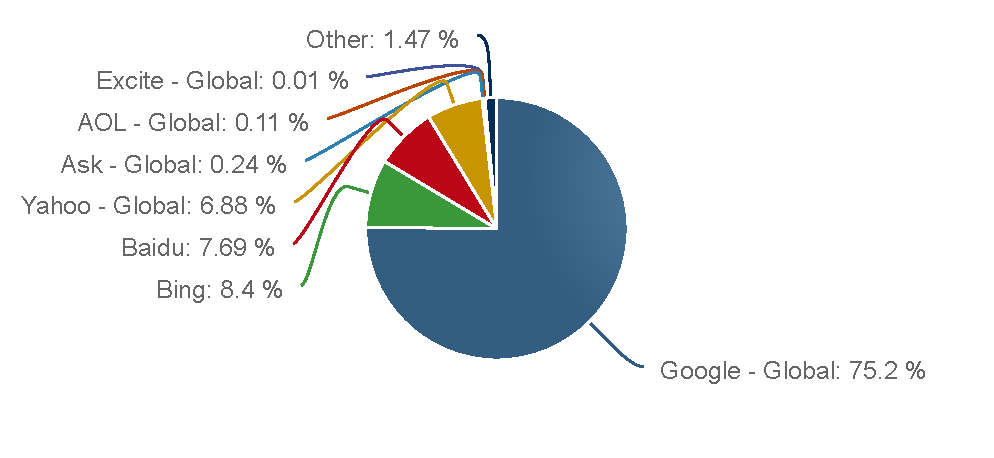
\includegraphics[width=\textwidth]{img/netmarketshare.pdf}
  \caption{Množství zpracovaných dotazů jednotlivými vyhledávači, zdroj: \url{www.netmarketshare.com}, 3.11.2016}
  \label{fig:netmarketshare}
\end{figure}

S rozvojem SEO technik se techniky začaly dělit na 2 tábory. \textbf{White-hat SEO}, které se zabývá formálními přístupy k vylepšení pozice mezi výsledky a \textbf{black-hat SEO}, které využívá mezer vyhledávacích algoritmů.

V této kapitole si představíme pohled na 3 subjekty, které přicházejí s vyhledáváním do styku - je to samotný \textbf{vyhledávač}, \textbf{uživatel} a \textbf{SEO}. Bude popsán způsob, jakým se vyhledávače vyvíjely ruku v ruce s tvorbou SEO technik a také to, jak se tyto dva tábory ve vývoji vzájemně podněcovali. Ukážeme si, jak funguje vyhledávač Google, na který se v této práci zaměřujeme. Musíme chápat, že \textbf{algoritmy tohoto vyhledávače nejsou volně přístupné}, avšak skrze informace, které Google zveřejňuje a skrze výzkum toho, jaké faktory ovlivňují umístění ve výsledcích vyhledávání, můžeme usuzovat, jak tento vyhledávač pracuje a můžeme pro něj optimalizovat. 

\newpage
\section{Webové vyhledávače}
\label{section:searchengines}
Prvních 20 let se tvůrci internetu zajímali spíše o jeho fyzickou infrastrukturu a to přineslo prudký rozvoj rychlostí a datových kapacit sítě. Tento prudký rozvoj s sebou přinesl odpovídající rozvoj v množství dostupných informací. Pro uživatele internetu bylo v tomto datovém oceánu čím dál tím složitější nalézt požadované informace. Uživatel typicky přistupoval k internetu přes poskytovatele služeb jako \textit{\textbf{USENET}}, \textit{\textbf{WHOIS}} a další komunitně specifické zdroje informací. Bez toho, aniž by informace o nových zdrojích (serverech) byla zveřejněna u poskytovatele takovéto služby, uživatel neměl možnost jak se dovědět o nově vzniklých zdrojích informací. Netrvalo to dlouho a začaly se objevovat první vyhledávače. Webový vyhledávač je softwarový systém, který byl navhrnut k vyhledávání informací v síti internetu. Webový vyhledávač prochází síť internetu a mapuje ji. Uživatel zadá do vyhledávače dotaz, který obsahuje popis toho co hledá, vyhledávač tento dotaz zpracuje a vrátí uživateli nejvíce relevantní výsledky, které ho nasměrují k požadované informaci. Výsledky mohou být mixem webových stránek, obrázků a dalších typů souborů - z tohoto důvodu se bavíme o univerzálních vyhledávačích.

Většina dnešních vyhledávačů funguje na základě \textbf{automatizovaných vyhledávacích algoritmů}, které prochází aktivní weby a vytváří si abstraktní reprezentaci webové topologie, kterou následně využívají v procesu zpracování uživatelských dotazů. Oproti této automatizaci stále nacházíme velké množství \textbf{webových adresářů}, které jsou ručně spravovány editory. Udržování takovýchto adresářů je časově mnohem náročnější a neumožňuje reagovat na růst, který world wide web od počátku nového tisíciletí zaznamenal. Vzhledem k cíli této diplomové práce se v následující kapitole nebudeme zabývat webovými adresáři, avšak pouze vývojem webových vyhledávačů, které fungují na základě určitých automatizovaných algoritmů a lze pro ně uplatnit SEO.

\newpage
\subsection{Historie vyhledačů}
\label{section:searchenginehistory}
Koncept \textit{\textbf{hypertextu}} a rozšíření lidské paměti sahá až do roku 1945. Prudký rozvoj technologií v průběhu druhé světové války s sebou přinesl také potřebu učinit získané informace člověku co nejvíce přístupné. \textbf{Dr. Vannervar Bush}, vedoucí oddělení pro vědecký výzkum a rozvoj, koordinoval ve válečném období práci více než 6000 vědců, mimo jiné také projekt Manhattan\footnote{\url{https://en.wikipedia.org/wiki/Manhattan_Project}}. Hned po válce, v roce 1945, vyzval v článku \textbf{As We May Think} \cite{aswemaythink} vědce k tomu, aby našli cestu, jak člověku přiblížit množství informací a rozšířit tak jeho sílu mysli. \\

Vannevar Bush píše:\\
\textit{\uv{Mendelův koncept zákonů genetiky byl ztracen po generaci, jelikož jeho publikace nedosáhla k těm několika, kteří byly schopní ho uchopit a rozšířit. Tyto katastrofy se bez pochyb kolem nás neustále opakují a nechávají tak zmizet to významné v záplavě nevýznamného.}}\cite{aswemaythink}
\\

Vannervar Bush také navrhl myšlenku neomezeného, rychlého, spolehlivého a rozšířitelného zařízení, které bude sloužit jako paměťové úložiště založené na asociativní paměti - stejně tak, jak ukládá informace člověk. Toto zařízení pojmenoval \textbf{Memex}.


Samotný termín hypertext však nepochází přímo od Bushe, avšak od \textbf{Teda Nelsona}. Ten v roce 1960 vytvořil \textbf{projekt Xanadu}, jehož cílem bylo vybudovat jednoduchou počítačovou síť s jednoduchým uživatelským rozhraním, která by řešila problém \textbf{autorství} a \textbf{odkazování}. Xanadu měl být univerzální knihovnou, celosvětovým publikačním systémem a také systémem pro diskuze a debaty. Systém byl navržen tak, aby se vyhnul složitému \textit{markupu} a tzv. mrtvým odkazům, které odkazují na určitý nedostupný dokument - tato vlastnost je něčím, co dnešní web postrádá. Dnešní web je postaven na odkazech, které jsou jednosměrné, avšak Xanadu počítal s \textbf{odkazy obousměrnými}. V síti s obousměrnými odkazy ví každý z uzlů sítě, kdo na něj odkazuje a je tak možné vytvořit celkovou síťovou topologii (abstraktní reprezentaci propojenosti sítě). Samotný projekt se nerozvíjel, avšak inspiroval mnoho svých následníků. Gary Wolf ve svém článku The Curse of Xanadu\footnote{\url{https://www.wired.com/1995/06/xanadu/}} napsal, že tento projekt byl nejdéle běžícím \textit{vaporwarem} s více než 30 lety vývoje. Přes všechnu kritiku, kterou Nelson sklidil, inspiroval tímto projektem mnoho svých následníků, mezi které patří také \textbf{Tim Berners Lee}, tvůrce \textbf{WWW} (kapitola \ref{section:WWW}). Pro bližší popis projektu Xanadu doporučuji knihy \cite{dreammachines} a \cite{literarymachines}.

\subsubsection{Archie}
Archie byl prvním vyhledávačem, který v roce 1990 vytvořil \textbf{Alan Emtage}, student McGill University v Montrealu. Archie neprocházel obsah souborů umístěných v síti tak, jak to dnes například dělá Google, avšak zjednodušil práci s protokolem \textit{\textbf{X.500}} a umožnil tak uživatelům internetu automatické indexování obsahu jejich \textit{FTP} serveru. Arhie se stal databází názvů souborů, které se porovnávaly s vyhledávaným dotazem.

\subsubsection{Veronica \& Jughead}
S roztoucí popularitou vyhledávače Archie jeho uživatelé hledali cesty k jeho vylepšení. Byl vytvořen vyhledávač Veronica, který fungoval podobně jako Archie - indexoval názvy a typy souborů na FTP serverech, avšak uměl také přímo procházet obsah textových souborů. Rozšířil tak možnosti o jednoduché \textit{fulltextové vyhledávání}.

\subsubsection{WWW}
\label{section:WWW}
Před nástupem World Wide Webu (WWW) sdíleli uživatelé sítě internet soubory pomocí FTP. Pokud jste chtěli sdílet nějaký soubor, zřídili jste si FTP server a lidé se k vám mohli připojit pomocí FTP klienta a tento soubor si stáhnout. Roku 1989 byl CERN největším evropským uzlem internetové sítě. \textbf{Tim Berners-Lee}, který dříve spolupracoval s \textbf{Robertem Caillaiau} na prototypu hypertextového systému s názvem \textbf{Enquire}, byl zaměstnancem Evropské organizace pro jaderný výzkum (CERN). Tim chtěl použít znalosti načerpané z tvorby Enquire a chtěl tento systém nasadit v CERNu pro sdílení informací mezi výzkumníky. Tim použil myšlenky systému Enquire, aby vytvořil World Wide Web, který sám navrhl a implementoval také první webový prohlížeč, editor a webový server, který nazval \textbf{httpd} (HyperText Transfer Protocol daemon). \\

Slovy Tima Berners-Lee: \\
\textit{\uv{Prostě jsem musel vzít myšlenku hypertextu a spojit ji s TCP a DNS a ta-dá! World Wide Web. Vytvoření webu byl akt zoufalství, jelikož bez něj byla práce v CERNu složitá. Většina technologií zahrnutá ve webu - hypertext, internet atd. již tou dobou existovala. Musel jsem to jen dát dohromady. Byl to krok generalizace. Krok k vyšší abstrakci, kde se všechny dokumentační systémy staly součástí imaginárního většího dokumentačního systému.}}\footnote{\url{http://www.achievement.org/autodoc/page/ber1int-1}}
\\

První webová stránka měla URL \url{http://info.cern.ch/} a byla spuštěna \textbf{6.8.1991}. Tato stránka obsahovala informace o tom, co je to World Wide Web, jak je možné nainstalovat webový prohlížeč a jak nainstalovat a nastavit webový server. Tato webová stránka byla také prvním adresářem, který spravoval sám Berners-Lee - \textbf{VLib}. Tim Berners-Lee také založil \textbf{W3C} (the World Wide Web Consortium) - mezinárodní komunitu, která vyvíjí otevřené standarty, aby zajistila dlouhodobý růst webu. 

\subsubsection{World Wide Web Wanderer}
V červnu roku 1993, vytváří \textbf{Matthew Gray} prvního \textbf{počítačového robota}. Počítačový robot je program, který urychluje opakující-se úkoly, které provádí rychlostí, kterou by člověk pracovat nemohl. Termín robot, nebo také \textbf{bot}, se v rámci internetu používá pro programy, které sbírají data z webových stránek. Vyhledávače používají roboty, kterým specificky říkají \textbf{spideři}. Jsou to programy, které si vyžádají stránky stejným způsobem, jako by to udělal uživatel skrze webový prohlížeč, přečtou obsah, analyzují ho a zaznamenají výsledek do \textbf{indexu}. Index je abstraktní reprezentace sítě, která slouží pro potřeby vyhledávání.  
Matthew Gray takového robota používá v projektu World Wide Web Wanderer\footnote{\url{http://www.mit.edu/~mkgray/net/background.html}}. Tento projekt měl za cíl měřit velikost WWW sítě pomocí počítačových botů, kteří procházeli aktivní web servery. Boti zachytávali \textit\textbf{{URL adresu}} webů a uchovávaly ji v databázi, která se stala známá jako \textbf{Wandex}. Aby byla tato databáze aktuální, přistupovaly boti na stejnou webovou stránku v řádech stovek návštěv denně, což způsobovalo značné zpomalení tehdejších serverů.\footnote{\url{http://www.searchenginehistory.com}}

\subsubsection{Aliweb}
Aliweb byl spuštěn v říjnu 1993 jako odpověď na problémy World Wide Web Wandereru. Aliweb procházel \textbf{meta informace} webů a umožňoval uživatelům, aby svůj web přihlásily k indexaci. Tím, že Aliweb používal pouze meta informace, snížil tak množství dotazů na servery a tudíž je tolik nepřetěžoval jako World Wide Web Wanderer. 

\subsubsection{Jednoduché webové vyhledávače}
V prosinci roku 1993 pak byly spuštěny 3 nové webové vyhledávače - \textbf{JumpStation}, \textbf{World Wide Web Worm (WWWW)} a \textbf{RBSE Spider}. Tyto vyhledávače procházely weby a indexovaly jejich \textit{\textbf{hlavičky}}. Problém JumpStationu a WWWW byl v tom, že na vyhledávaný dotaz zobrazoval výsledky v pořadí, ve kterém byly weby indexovány. Toto řešil RBSE Spider, který implementoval jednoduchý \textbf{hodnotící systém (ranking system)}, na základě kterého \textbf{vyhodnocoval relevantnost výsledků} vůči uživatelskému dotazu. 

\subsubsection{WebCrawler}
V dubnu roku 1994 spustil \textbf{Brian Pinkerton} z University of Washington vyhledávač, který pojmenoval WebCrawler. Během krátké chvíle se stal tak populárním, že se kvůli počtu uživatelských dotazů stal nepoužitelným. Popularita WebCrawleru byla zapříčiněna tím, že vyhledávač \textbf{indexoval kompletní weby} - nejen hlavičku a meta informace, avšak také jejich obsah. Jedná se tak o \textbf{počátek fulltextového vyhledávání}. WebCrawler byl odpokoupen společností \textbf{AOL}, která ho začlenila do své sítě. Význam WebCrawleru je hlavně ten, že inspiroval ke vzniku dalších projektů - \textbf{Lycos}, \textbf{Infoseek} a \textbf{OpenText}.

\subsubsection{Lycos}
Tento vyhledávač vznikl v červnu 1994 na Carnegie Mellon University. Lycos implementoval hodnotící systém a implementoval sémantickou analýzu \textbf{vzdáleností slov na webových stránkách} pro lepší pochopení obsahu indexovaných stránek. Hlavním rozdílem a konkurenční výhodou Lycosu však byla \textbf{velikost jeho databáze}. V dubnu roku 1994 indexoval 394 000 dokumentů, v lednu 1995 pak 1,5 milionu a v listopadu 1996 více než 60 milionů dokumentů - více než jakýkoliv jiný webový vyhledávač tou dobou. Tehdejším majoritním vyhledávačem \textbf{Netscape} byl Lycos ohodnocen jako nejlepší vyhledávač v počtu nalezených relevantních odkazů na vyhledávaný řetězec \uv{surf}.\footnote{http://www.searchenginehistory.com}

\subsubsection{Infoseek}
Infoseek byl vyvíjen od roku 1994. Tento vyhledávač nepřinášel příliš mnoho inovací, avšak jeho důležitost značně stoupla ve chvíli, kdy jeho představitelé přesvědčily společnost Netscape, aby ve svém webovém prohlížeči používala tento vyhledávač jako primární. Jednou z novinek tohoto vyhledávače byla \textbf{možnost odeslat webovou stránku k indexaci v reálném čase}, což se nakonec ukázalo jako zcestné, jelikož toho s oblibou využívali spammeři. 

\subsubsection{AltaVista}
AltaVista byla revolučním vyhledávačem spuštěným roku 1995, který umožňoval \textbf{vy\-hle\-dá\-vá\-ní pomocí dotazů v přirozeném jazyku}, přinášel \textbf{komplexní dotazy} a také umožňoval uživateli \textbf{přidat a odebrat webové stránky během 24 hodin}. AltaVista ztroskotala díky špatnému managementu a manipulaci výsledků. V době, kdy se pak objevil Google a Inktomi, byla AltaVista mnohem horší ve zpracování dotazů a v poskytování relevantních výsledků. AltaVista byla roku 2003 koupena společností \textbf{Overture}, která byla následně koupena společností Yahoo a vyhledávač AltaVista se tak stal součástí vyhledávače \textbf{Yahoo! Search}. 

\subsubsection{Inktomi}
Vyhledávač \textbf{Hotbot} společnosti Inktomi spatřil světlo světa 20.5.1996 a získal si velmi rychle přízeň velké skupiny uživatelů. Novinkou, kterou Inktomi přineslo byl \textbf{model PPC reklamy}. Inktomi ztratilo většinu uživatelů po \textbf{dot-com bublině}\footnote{\url{https://en.wikipedia.org/wiki/Dot-com_bubble}} a v prosinci roku 2003 bylo prodáno společnosti Yahoo.

\subsubsection{Ask.com (Dříve Ask Jeeves)}
V dubnu 1997 byl spuštěn vyhledávač Ask Jeeves, který \textbf{dokázal zpracovat dotazy zadáva\-né v přirozené řeči}. Vyhledávač implementoval hodnotící systém \textbf{DirectHit}, který hodnotil výsledky vyhledávaní \textbf{podle popularity}. Tento systém byl však jednoduše zneužitelný spammery. DirectHit byl později nahrazen hodnotím systémem \textbf{Teoma}, který některé z těchto nedostatků řešil.

\subsubsection{Meta vyhledávače}
Většina meta vyhledávačů získává své výsledky skrze množinu jiných vyhledávačů, \textbf{kombinují jejich výsledky a pomocí vlastního hodnotícího systému je ohodnotí}. Meta vyhledávače byly populární v dobách, kdy byla indexace stránek internetu systémově náročnou operací a nebyla tak efektivní. Kombinací výsledků různých vyhledávačů bylo dosaženo vysoké efektivity při nízkých systémových nárocích (outsourcing).

\subsubsection{Yahoo!}
Yahoo! bylo založeno roku 1994 jako \textbf{webový adresář}. Dlouhou dobu se Yahoo soustředilo pouze na svůj adresář a vyhledávání \textit{outsourcovalo}. Koncem roku 2002 si Yahoo uvědomilo důležitost vyhledávání, koupilo \textbf{Inktomi} a následně v červnu 2003 společnost \textbf{Overture}, která již dříve koupila \textbf{AllTheWeb} a \textbf{AltaVistu}. 29.června 2009 se Yahoo! rozhodlo, že se vzdá svých ambicí na poli vyhledávačů a podepsalo smlouvu s výhledávačem \textbf{Bing}, který od té chvíle dodává pro Yahoo výsledky hledání\footnote{\url{http://searchenginehistory.com}}.

\subsubsection{Google}
\label{section:historyofgoogle}
Google je mezinárodní společnost specializující se na internetové služby a produkty, které zahrnují reklamu, vyhledávání, výpočetní cloud a software. Většina přijmů Googlu vychází ze systému \textbf{AdWords}, který umisťuje reklamu poblíž výsledků vyhledávání.\footnote{\url{https://abc.xyz/investor/index.html}}. Z hlediska vývoje SEO technik je důležité znát historii vývoje vyhledávače Google. Techniky přicházely a odcházely tak, jak Google aktualizoval své algoritmy. (Přehled aktualizací v příloze \ref{app:GoogleUpdates}). Pro podrobnou historii společnosti Google doporučuji \url{https://www.google.com/about/company/history}.

V lednu 1996 začali \textbf{Larry Page} a \textbf{Sergey Brin} pracovat na vyhledávači pojmenovaném \textbf{BackRub}. Název vycházel z toho, že vyhledávač analyzoval zpětné odkazy a hodnotil webové stránky tak, že upřednostňoval ty, na které bylo hodně odkazováno - podobně jako se hodnotí články v akademické obci, ze které Larry i Sergey vzešli. Algoritmus, který takto stránky hodnotil byl pojmenován \textbf{PageRank} (ze jména Larryho Page). (O PageRanku více v kapitole \ref{section:pagerank}). Sergey se pokusil technologii PageRanku prodat, avšak nikdo neměl o koupi či licencování zájem.\footnote{\url{http://www.searchenginehistory.com}} 

\begin{figure}
  \centering
    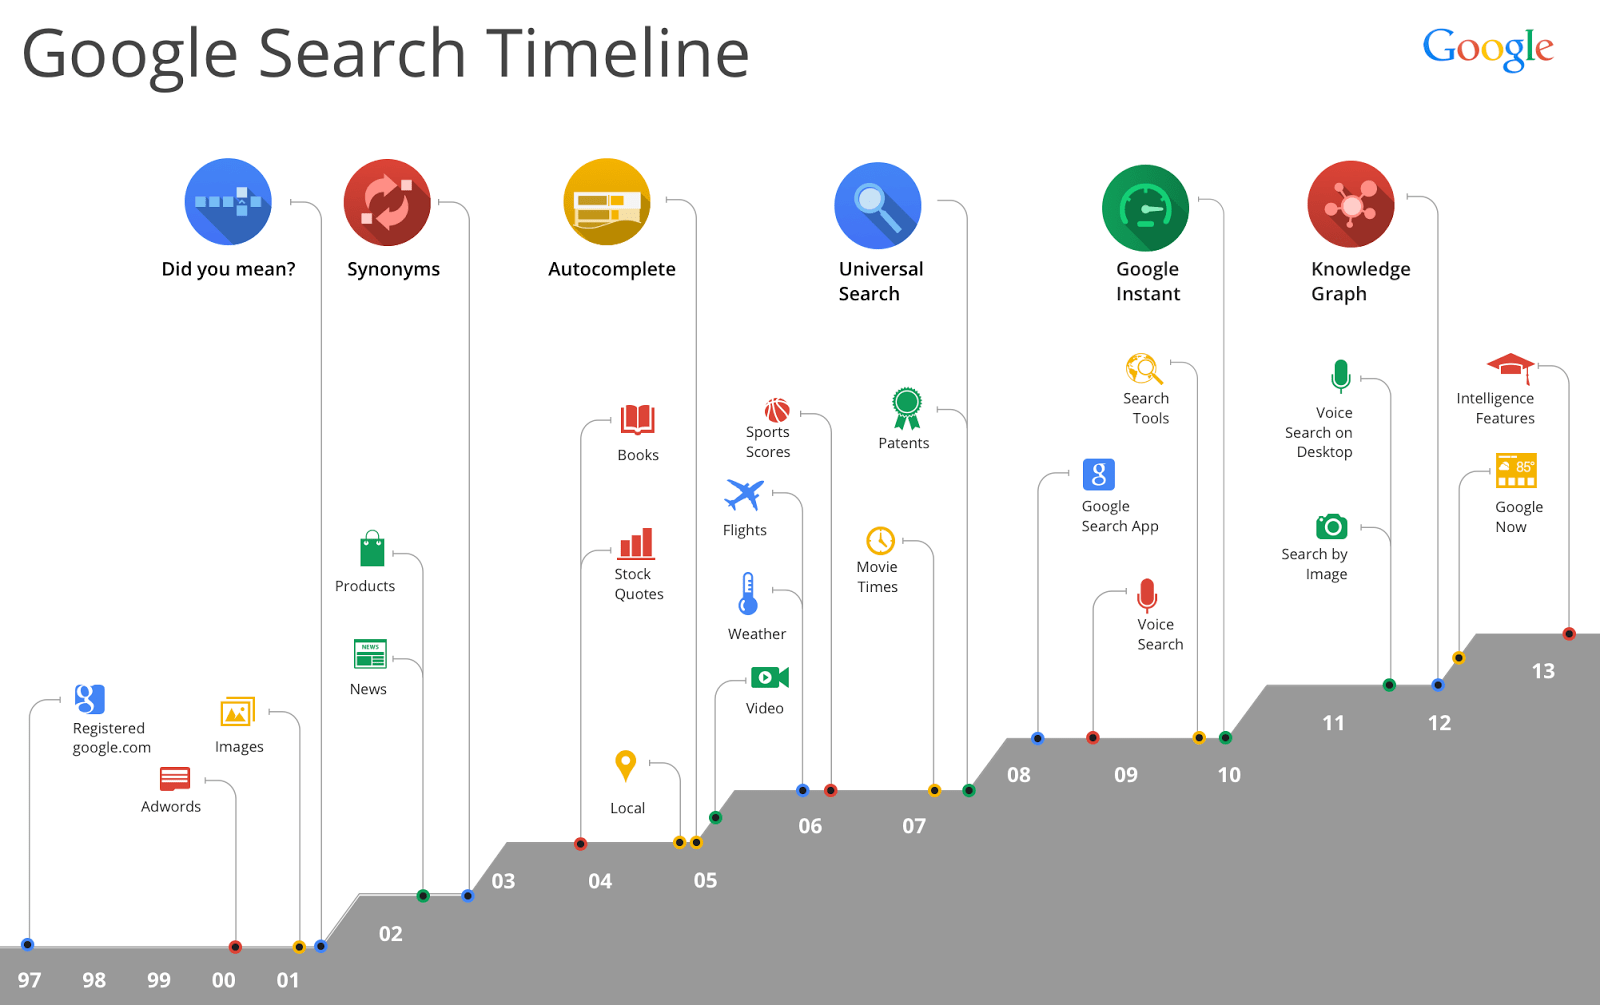
\includegraphics[width=\textwidth]{img/searchtimeline.png}
  \caption{Historie vývoje vyhledávače Google, Zdroj: Google Search Official Blog}
  \label{fig:searchtimeline}
\end{figure}

15. Září 1997 byla registrována doména \url{google.com}, jejíž název vychází z matematického výrazu \textbf{googol}, což je výraz pro číslo 1 následované stem nul\footnote{\url{https://en.wikipedia.org/wiki/Googol}} a má vystihovat Larryho a Sergejovo poslání \textbf{uspořádat zdánlivě nekonečné množství informací na internetu}\footnote{\url{https://www.google.com/about/company/history/}}. Spoluzakladatel společnosti Sun, \textbf{Andy Bertolsheim}, vypisuje v srpnu 1998 šek na 100 000\$ a 4.září je pak založena společnost Google. V prosinci 1998 časopis \textbf{PC Magazine} uvádí, že Google \textit{\uv{má nadpřirozenou schopnost vracet extrémně relevantní výsledky}}, a ve výběru 100 nejlepších webových stránek pro rok 1998 ho oceňuje jako vybraný vyhledávač\footnote{\url{https://web.archive.org/web/19990508042436/www.zdnet.com/pcmag/special/web100/search2.html}}. V květnu 2000 je uvedeno prvních deset jazykových verzí a v září již počet jazykových verzí narůstá na 15. V říjnu 2000 je uvedena služba \textbf{AdWords}, samoobslužný reklamní systém. Roku 2003 pak Google spustil službu \textbf{AdSense}. Následovalo spuštění mnoha služeb jako např. \textbf{Google News}, \textbf{Book Search}, \textbf{Scholar}, \textbf{Blog Search}, \textbf{Gmail}, \textbf{Maps}, \textbf{Calendar} atd. Tyto služby upevnily postavení Googlu na trhu, avšak pro tuto diplomovou práci nejsou sami o sobě podstatné. Jejich důležitost tkví především v tom, že Google takto získal množství informací, které používá v rámci svého vyhledávání. Důležitou službou se roku 2005 stalo \textbf{Google Analytics} (více o nástroji v kapitole \ref{section:analytics}). Analytics pomáhá \textit{webmasterům} ke sledování publika a návštěvnosti webů, což je pro SEO velmi důležité. Další službou, která je uřčena pro webmastery je \textbf{Google Webmaster Tools} (kapitola \ref{section:webmaster}). Tato služba umožňuje přihlásit web k indexování, sledovat kolik stránek bylo naindexováno a pomáhá odhalit chyby, které mohou při indexaci vzniknout. Roku 2006 koupil Google \textbf{Youtube} - největší portál s videi a přidal tak do svého vyhledávání nový zdroj informací. V roce 2009 provedl Google tzv. \textbf{Vince update}, v roce 2011 přišel Google s \textbf{Panda algoritmem} a v roce 2012 s \textbf{Penguin update} (přehled aktualizací v příloze \ref{app:GoogleUpdates}, popis v následujících kapitolách). Těmito aktualizacemi odstranil mnoho spamových stránek, kterých je world wide web plný. V roce 2008 google zpracovával 1 trillion stránek, v současnosti Google zpracovává \textbf{130 trillionů}\footnote{\url{https://www.google.com/insidesearch/howsearchworks/thestory/}} stránek na webu. Jak je vidět, rozvoj webu je velmi rychlý. Způsob, jakým vyhledávač Google pracuje, je popsán v kapitole \ref{section:anatomy}

\subsubsection{Bing}
Historie vyhledávače Bing se datuje do roku 1998, kdy Microsoft spustil \textbf{MSN Search}. Z počátku Microsoft nebral vyhledávání moc vážně, ale ve chvíli, kdy se osvědčil obchodní model Googlu, začal se na vyhledávání více soustředit. 31.1.2005 začal MSN Search používat svou vlastní vyhledávací technologii a odprostil se tak od Yahoo!. 1.6.2009 spustil Microsoft vyhledávač \textbf{Bing}, který do výsledků vyhledávání začal přidávat výsledky příbuzné s vyhledávaným řetězcem. Pokud tak uživatel vyhledával například řetězec \uv{kreditní karty}, přidal vyhledávač Bing výsledky hledání z řetězců \uv{typy kreditních karet}, \uv{žádost o kreditní kartu} a další. Bing nyní (listopad 2016) obsluhuje 8,4 \% všech vyhledávacích dotazů a zaujímá tak druhé místo na trhu vyhledávačů. Algoritmy vyhledávače Bing jsou v mnohém velmi podobné algoritmům vyhledávače Google a SEO techniky, které si uvedeme v kapitole \ref{section:SEO} jsou platné jak pro Bing tak i pro Google. 

\subsection{Anatomie vyhledávače}
\label{section:anatomy}
Předtím než může vyhledávač říci, kde se který dokument v síti nachází, musí být dokument nalezen. Aby vyhledávač získal informace z trilionů webových stránek\footnote{\url{https://www.google.com/insidesearch/howsearchworks/thestory/}}, nasazuje na vyhledání specialní softwarové roboty. Pro tyto roboty se často používá název \textit{\textbf{spideři}}, nebo také \textit{\textbf{boti}}. Proces procházení webů se nazývá \textit{\textbf{crawling}}. Informace získané ze stránek jsou uloženy v \textit{\textbf{indexu}}. Když potom vyhledáváte pomocí vyhledávače, neprohledáváte celou WWW síť, ale procházíte indexem, který si vyhledávač spravuje. Třetí částí vyhledávače je pak vyhledávací rozhraní skrze které uživatel zadává dotazy.

\begin{figure}
  \centering
    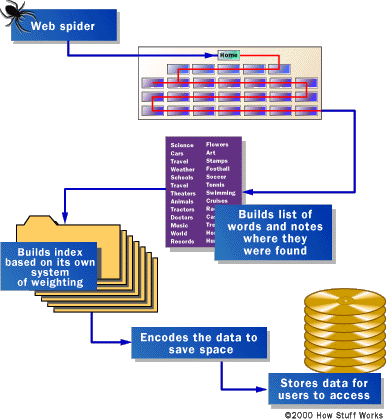
\includegraphics[width=\textwidth]{img/anatomy.png}
  \caption{Anatomie vyhledávače, zdroj: \url{http://computer.howstuffworks.com/internet/basics/search-engine1.htm}}
  \label{fig:anatomy}
\end{figure}

\subsubsection{Crawling a indexace}
K poskytnutí nejlepších výsledků se vyhledávače pokouší nalézt všechny veřejně dostupné stránky a dokumenty na internetu a snaží se prezentovat ty nejvíce relevantní k uživatelskému vyhledávacímu dotazu. Prvním krokem vyhledávače je procházení (crawling). Webové vyhledávače začínají s \textbf{množinou vysoce kvalitních webů} a postupně navštěvují všechny stránky, na které se z těchto kořenových webů odkazuje. Procházení má \textbf{\textit{rekurzivní} charakter} a pokračuje z odkazů na stránkách v druhé úrovni od kořenových, následně ve třetí atd. Spideři, kteří přes tyto odkazy procházejí zdrojový kód stránek, analyzují jejich obsah (kapitola \ref{section:onpageanalysis}) za cílem vybudování indexu. Index je masivní databáze, která je neustále aktualizována prací spiderů. Kvalita indexovací technologie má přímý dopad na přesnost a odezvu výhledávačů \cite{Fishkin2015}.

V průběhu analýzy se buduje \textbf{sémantická mapa}, která definuje vztahy mezi koncepty, kterým je vyhledávač schopen porozumět. Analyzovaná stránka je \textbf{rozdělena na bloky} jako navigace, obsah, patička, tagy, komentáře, atd. Vyhledávače se primárně soustředí na obsah samotný a obsažená klíčová slova. Na obrázku \ref{fig:vseblocks} lze vidět příklad rozdělení stránky pro potřeby analýzy. Unikátním obsahem, který zde vyhledávač primárně analyzuje, je blok \uv{Profil fakulty}. Menu, logo, hlavička samotného webu, vyhledávání a další elementy nejsou pro analýzu tak důležité jako právě unikátní obsah v hlavním bloku \cite{Enge2015}. Pro rychlý přístup k informacím vytváří vyhledávač Google při indexaci stránek také tzv. \textbf{knowledge graph} (kapitola \ref{section:knowledgegraph}), který se následně používá pro rychlé zodpovězení otázek a pro rychlý přehled informací o daném tématu přímo v prostředí vyhledávače. 

\begin{figure}
  \centering
    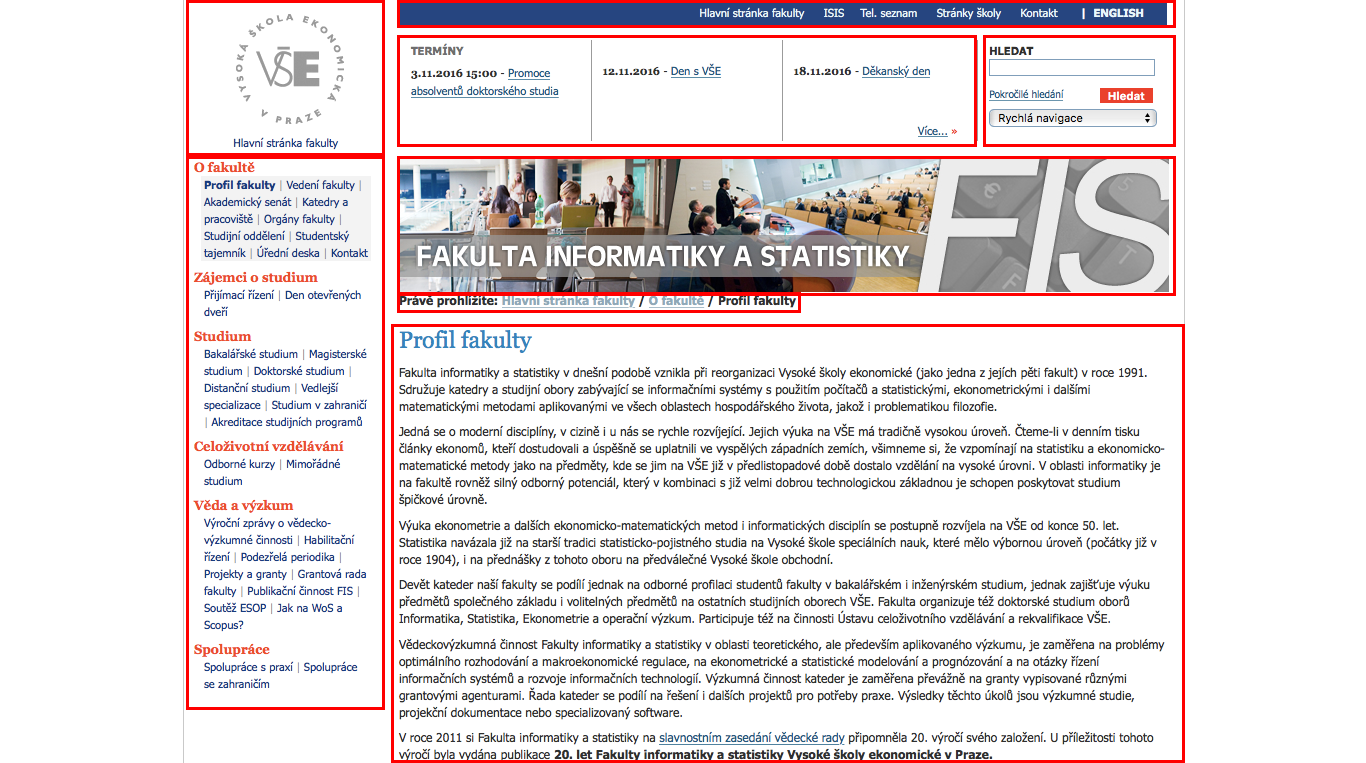
\includegraphics[width=\textwidth]{img/vseblocks.png}
  \caption{Ukázka rozdělení webové stránky na bloky určené k analýze vyhledávačem, zdroj: \url{vse.cz}}
  \label{fig:vseblocks}
\end{figure}

\newpage
\subsubsection{Vyhledávací algoritmy}
\label{section:signals}
Pro běžný dotaz jsou k dispozici tisíce, ne-li milióny webových stránek s užitečnými informacemi. Uživatel však hledá odpověď, nikoliv miliony webových stránek. Vyhledávačům jde hlavně o \textbf{relevanci}, neboli úroveň, ve které koresponduje uživatelský dotaz s poskytnutými výsledky. Relevantnost souvisí také s důležitostí obsahu. V akademické obci jsou důležité ty články, které jsou často citované. Stejně tak je tomu i při vyhledávání. Čím více odkazů vede na daný dokument či webovou stránku, tím je relevantnějším zdrojem informací. Důležitost ani relevantnost \textbf{nejsou hodnoceny manuálně}, avšak slouží k tomu algoritmy, které jednotlivé dokumenty a webové stránky ohodnocují (\textit{\textbf{ranking}}) a určují tak pořadí, ve kterém se výsledky vyhledávání zobrazí. Algoritmy se neustále aktualizují, aby poskytovaly co nejvíce relevantní výsledky a také bojují se spammery, kteří jsou čím dál tím více sofistikovaní. V příloze \ref{app:GoogleUpdates} je uveden přehled nejdůležitějších aktualizací algoritmů vyhledávače Google. U některých z nich si v této práci ukážeme jejich funkci. 
 
Současné algoritmy vyhledávače Google vycházejí z \textbf{více než 200 jedinečných signálů}\footnote{\url{https://www.google.co.uk/insidesearch/howsearchworks/algorithms.html}} neboli vodítek, pomocí kterých lze odhadnout, co asi ve skutečnosti hledáte. Je důležité zmínit, že \textbf{zdrojový kód vyhledávacích algoritmů není volně k dispozici}. SEO specialista, který se snaží dostat své stránky mezi přední pozice, musí optimalizovat krokově a sledovat jakým způsobem se mění umístění optimalizovaného webu a přistupovat tak k vyhledávači jako k \textit{\textbf{šedé skříňce}}\footnote{\url{https://en.wikipedia.org/wiki/Gray_box_testing}}, o které něco málo ví, avšak není schopen se podívat na její přesnou funkci a najít trvalé optimalizační maximum. 

\subsubsection{Vyhledávací rozhraní}
\label{section:searchui}

Vyhledávače indexují širokou škálu datových typů: text (blogové příspěvky, články, osobní weby, ...), rss kanály, videa, obrázky a také \texttt{PDF} a \texttt{mp3} soubory. Vyhledávače v průběhu let získaly jejich používaností mnoho uživatelské zpětné vazby a optimalizovali tak své rozhraní k maximální efektivnosti ve vyhledávání a \textbf{UX} (\textbf{U}ser E\textbf{x}perience). Změny UI a přizpůsobování uživateli je neustálé. Od čistě textových výsledků vyhledávače přešly na vyhledávání skrze mnoho médií, rozvinuly sémantičnost sítě WWW a přiblížily se tak fungování lidské asociativní paměti a lidským myšlenkovým konceptům. Na některé vyhledávací řetězce lépe odpoví video, na některé text na Wikipedii a na jiné zase PDF soubor či obrázek. Vyhledávač, který takto kombinuje výsledky různých datových typů se označuje jako univerzální vyhledávač. 

Na obrázku \ref{fig:mozmegaserp} je vidět možná kombinace výsledků různých typů. Typů výsledků je však ještě mnohem více\footnote{\url{https://moz.com/blog/mega-serp-a-visual-guide-to-google}}.

\begin{figure}
  \centering
    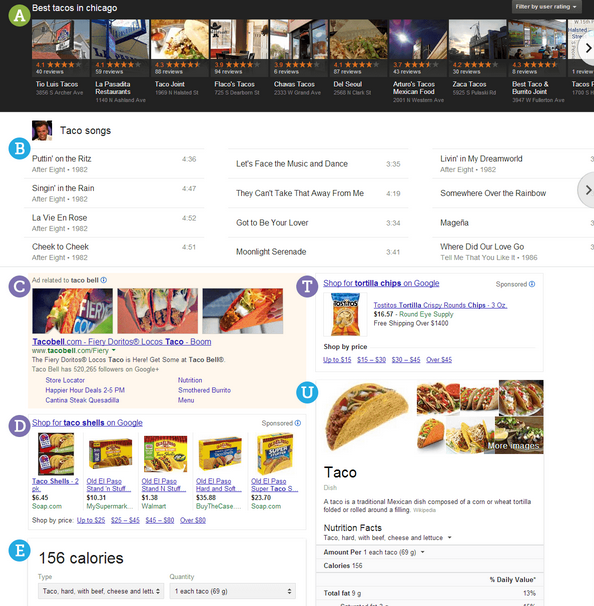
\includegraphics[width=\textwidth]{img/mozmegaserp.png}
  \caption{Možná kombinace výsledků různých datových typu na Google.com, zdroj: \url{moz.com}}
  \label{fig:mozmegaserp}
\end{figure}

\begin{enumerate}[label=(\Alph*)]
	\item Slider s lokálnímy výsledky 
	\item Slider s hudebnímy výsledky
	\item AdWords reklama
	\item Výsledky vyhledávání produktů 
	\item Box s odpověďmi
	\item Výsledky vyhledávání produktů
	\item Výsledky knowledge graphu 
\end{enumerate}

\subsubsection{Příklad vyhledávání v Google}

\begin{figure}
  \centering
    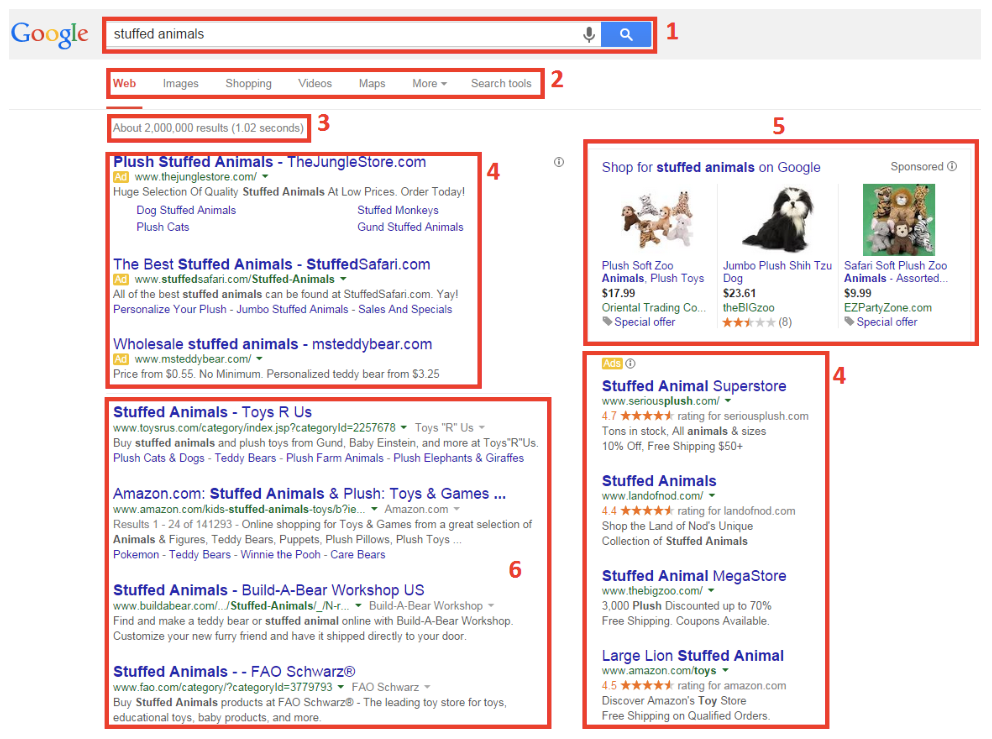
\includegraphics[width=\textwidth]{img/googlesearchexample.png}
  \caption{Příklad vyhledávání na Google.com, zdroj: google.com}
  \label{fig:googlesearchexample}
\end{figure}

Vyhledávač vrací výsledek v podobě \uv{\textbf{S}earch \textbf{E}ngine \textbf{R}esult \textbf{P}age} (SERP). Každý z vyhledávačů má drobně odlišný layout, avšak většina používá vertikální zobrazení. Na obrázku \ref{fig:googlesearchexample} můžeme vidět příklad vyhledávání ve vyhledávači Google. Rozdělení výsledků je ná\-sle\-do\-vné:

\begin{enumerate}
	\item Vyhledávací formulář
	\item Navigace
	\item Výsledky
	\item PPC reklama
	\item Sponzorované výsledky vyhledávání
	\item Organické výsledky vyhledávání
\end{enumerate}

\textbf{Za zobrazení PPC reklamy a sponzorovaných výsledků vyhledávání musíme zaplatit}. Google musí vědět při které kombinaci klíčových slov má propagovaný obsah zobrazit. Oproti organickým výsledkům však u PPC reklamy nezáleží na obsahu stránky. Výsledek PPC reklamy je pouze dočasný, avšak je zaručený. Odkaz na stránky je odstraněn po vyčerpání kreditu. Pokud je propagované klíčové slovo silně konkurenční, bude cena za PPC reklamu vysoká. 

\newpage
\subsection{Analýza a ohodnocení stránek}
Mezi signály vyhledávače pro ohodnocení patří informace získané z předchozích analýz zdrojových souborů stránek, ale také ty, které vyhledávač získá tím, že si buduje abstrakní reprezentaci WWW sítě  (například \textbf{hodnocení PageRank}\footnote{\url{https://www.google.com/insidesearch/howsearchworks/algorithms.html}}, nebo algoritmy, které dokáží posoudit např. \textbf{aktuálnost obsahu} a zjistit, co zrovna \uv{hýbe světem}\footnote{\url{https://www.google.com/trends/}}. 

Analyzuje se velké množství faktorů, které následně představují signály pro posouzení relevantnosti výsledků vyhledávání a zobrazit tak ty, které pravděpodobně zodpoví uživatelský dotaz. Důležitost jednotlivých signálů je při ohodnocování výsledků vyhledávání různá. Podle studie \cite{Dean2016} provedené v roce 2016 a také \cite{Hussien2014} z roku 2014 je možné usuzovat jaké signály jsou pro ohodnocení výsledků vyhledávání nejdůležitější. 
 
 \textbf{Bylo zjištěno, že}:
 \begin{itemize}
 	\item \textbf{Zpětné odkazy} (backlinks) jsou extrémně důležitým hodnotícím faktorem. Ve vý\-sled\-cích studií pořadí mezi výsledky vyhledávání silně korelovalo s množstvím zpětných odkazů. Důležitý je také počet domén, ze kterých odkazy směřují - pro lepší ohodnocení je mnohem důležitější mít 10 odkazů z 10 různých domén než 10 odkazů z 1 domény. (viz obr. \ref{fig:domainslinks} a algoritmus PageRank (kapitola \ref{section:pagerank}))
 	\item \textbf{Doména}, na které se nacházejí jednotlivé stránky je důležitější než samotné jednotlivé stránky. Nově zveřejněné stránky v rámci domény těží ze hodnoty této domény (z toho, že už je doména dlouhou dobu aktivní a že např. pravidelně přináší kvalitní obsah). 
 	\item \textbf{Tématická relevance} příspěvků na stránkách značně vyzdvihuje příspěvky, které hloubkově popisují dané téma. Je tedy vhodné psát obsáhlejší články, které se soustředí na jedno téma. Toto je způsobeno přichodem Hummingbird algoritmu - viz příloha \ref{app:GoogleUpdates} a kapitola \ref{section:hummingbird}. Průměr nejlépe hodnocených výsledků je 1890 slov na příspěvek.
 	\item Použití bezpečného \textbf{\textit{HTTPS}} protokolu silně koreluje s lepším ohodnocením.
 	\item \textit{\textbf{Schema markup}} nekoreluje s lepším ohodnocením.
 	\item Obsah s alespoň jedním \textbf{obrázkem} jednoznačně získává lepší ohodnocení. Další obrázky však již ohodnocení neovlivňují. 
 	\item Oproti očekávání nemá \texttt{<title>} tag takovou váhu. Toto je zřejmě způsobeno přesunem googlu k sémantickému vyhledávání (viz aktualizace vyhledávače - příloha \ref{app:GoogleUpdates}) a \ref{section:hummingbird}.
 	\item Byla odhalena silná pozitivní korelace mezi \textbf{rychlostí načítání stránek} a ohodnocením.
 \end{itemize}
 
 \begin{figure}
  \centering
    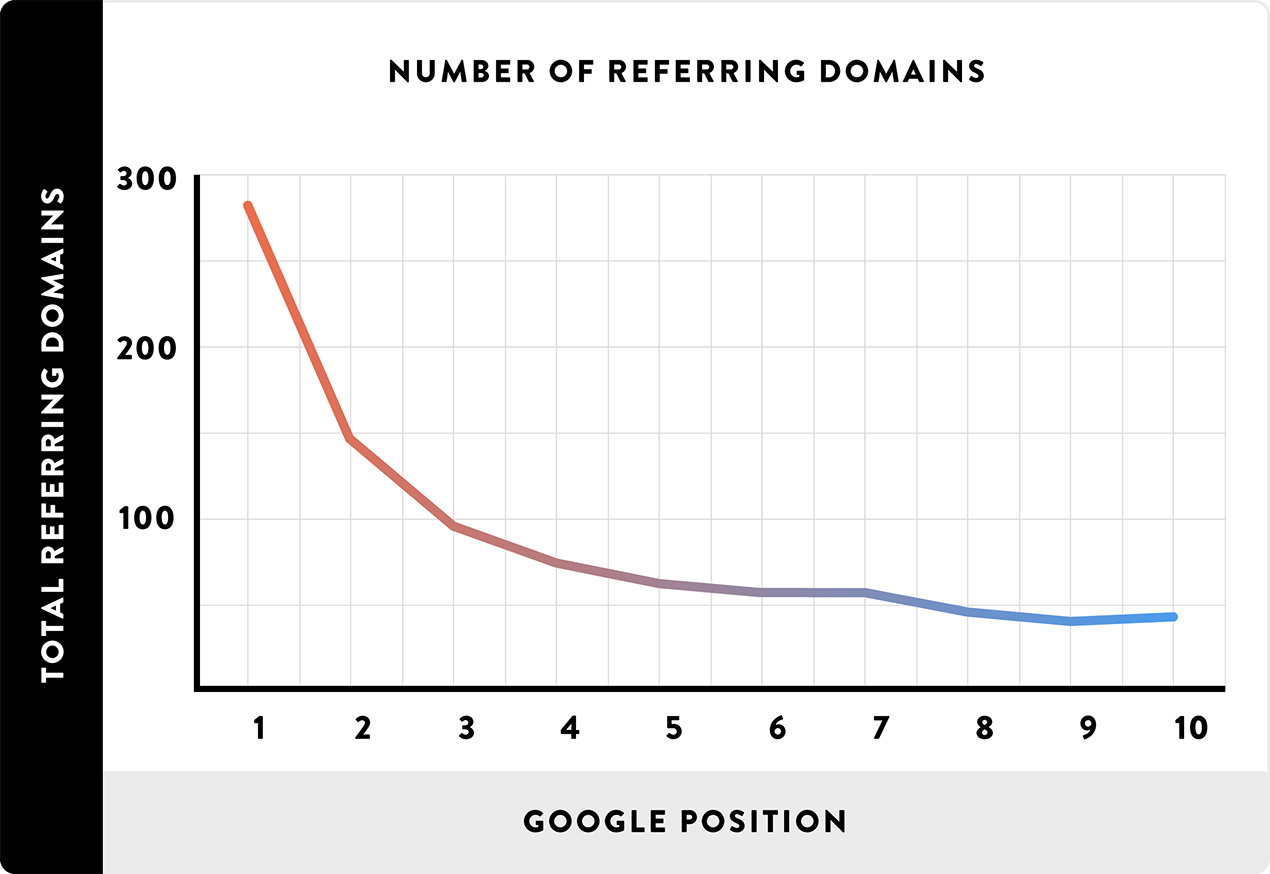
\includegraphics[width=\textwidth]{img/domainslinks.png}
  \caption{Závislost mezi počtem domén, ze kterých se odkazuje a pořadím ve výsledcích vyhledávače Google, zdroj: Backlinkto.com}
  \label{fig:domainslinks}
\end{figure}

\textbf{Analýza je rozdělena do několika částí}:
\begin{itemize}
	\item \textbf{\uv{On-Page} analýza} - Analyzuje informace dostupné přímo ve zdrojovém kódu stránky - nejde tak o vyhodnocení počtu odkazů směřujících na stránku, nebo o analýzu pro\-vá\-za\-no\-sti se sociálními sítěmi, ale především o klíčová slova obsažená v \texttt{<title>} a \texttt{<meta>} HTML tagu a o klíčová slova a odkazy v hlavním obsahovém bloku.
	\item \textbf{\uv{Off-Page} analýza} se zajímá o to, jak jsou dané webové stránky začleněny do sítě internetu - kdo na tyto stránky odkazuje, nebo jak je tato stránka populární na sociálních sítích.
	\item \textbf{Analýza webu jako celku} - Vyhledávače se zajímají o to, kde je umístěn server, na kterém je web umístěn, zda je web optimalizovaný pro mobilní zařízení, nebo zda je daný web přidán do Google Analytics či Google Webmaster Tools.  
	\item \textbf{Analýza domény} - Jak dlouho je spuštěna doména webu, jaká je historie domény a o jakou doménu se jedná (.com, .cz, .uk, .gov, .edu, ...). Obecně mají domény \texttt{.edu} a \texttt{.gov} velkou sílu při ohodnocování.
\end{itemize}

\subsubsection{\uv{On-Page} analýza}
\label{section:onpageanalysis}

\textbf{Analýza klíčových slov}
\label{section:keywordanalysis}

Moderní vyhledávače \textbf{sémanticky analyzují obsah stránek}, aby zjistili jaký typ informace se na stránkách nachází a aby porozuměly jeho významu. Pokud například vyhledávač nalezne slovo \uv{aloha}, asociuje toto slovo s Hawaií a ne s Floridou. Vyhledávače si aktivně vytvářejí vlastní \textbf{slovníky}, dle kterých určují k jakému tématu se váží určitá slova \cite{Enge2015}. Vyhledáváním v těchto slovnících a použitím \textit{\textbf{fuzzy logiky}} mohou rozumět webu podobným způsobem, kterým mu rozumí lidé. Analýza propojenosti slov může vyhledávači odhalit, že pomeranč je oproti banánu kulatý, jelikož se slova \uv{kulatý} a \uv{pomeranč} často vyskytují blízko sebe. Vyhledávač tak může říci, že pokud se vyhledává \uv{výlet do zoo}, bude k danému vyhledávání relevantní také vyhledávání \uv{zvířata}, nebo také \uv{cestování} \cite{Hussien2014}\cite{Fishkin2015}. Velký rozvoj sémantické analýzy doznal vyhledávač Google s tzv. \textbf{Hummingbird aktualizací} (viz kapitola \ref{section:hummingbird} a příloha \ref{app:GoogleUpdates}).

Korelace \textbf{klíčových slov obsažených v \texttt{<title>} HTML tagu} jsou i přes zjištění uvedené v předchozí části stále jedním z nejsilnějších signálů vyhledávače. Tag samotný je určen ke stručnému a přesnému popisu obsahu webové stránky. Vyhledávače využívají obsahu v tomto tagu k zobrazení titulku stránky v seznamu výsledků. Skrze \texttt{<title>} tag sdělujeme vyhledávači, na která klíčová slova se zaměřujeme. První slovo v tomto tagu získává největší pozornost \cite{Fishkin2015}.

\textbf{Klíčová slova v \texttt{<meta name='keywords' >} tagu} již dnes nemají takový význam - tento tag byl zneužíván k tzv. \uv{keyword stuffingu} a vyhledávače značně snížily jeho význam při ohodnocování \cite{Fishkin2015}.

\textbf{Klíčová slova v \texttt{<H1>} tagu} slouží jako další signál k určení relevance stránky. Obsah \texttt{<H1>} tagu je chápán jako popis stránky a je vhodné zde uvádět klíčová slova, na která se zaměřujeme.\\

\textbf{Google Hummingbird aktualizace}
\label{section:hummingbird}

Hummingbird aktualizace byla představena v září 2013 a zaměřuje se na sémantické vyhledávání - specificky na kontext a synonyma. Pomocí tohoto algoritmu lze lépe zjistit záměr vyhledávání\footnote{\url{https://moz.com/blog/hummingbird-unleashed}}. Hummingbird se více zaměřuje na jednotlivá slova a analyzuje jejich možné synonymní kombinace k tomu, aby mohl více porozumět samotnému sémantickému významu vyhledávání. Stejně tak jako knowledge graph (kapitola \ref{section:knowledgegraph}) se Hummingbird snaží \uv{pochopit} lidské myšlenkové koncepty a vztahy mezi klíčovými slovy\footnote{\url{http://www.bbc.co.uk/news/business-24292897}}. \\

\textbf{Analýza kvality a unikátnosti}

Vyhledávače se také zaměřují na \textbf{kvalitu} a \textbf{unikátnost} obsahu. Kvalita se dá např. jednoduše posoudit tím, že vyhledávač spočítá \textbf{počet gramatických chyb} a z toho usoudí, že si autor s obsahem nedal moc práce. Dalším krokem je \textbf{analýza náročnosti textu}. Ta se dá provést \textbf{Flesch-Kincaidovým}\footnote{\url{https://en.wikipedia.org/wiki/Flesch–Kincaid_readability_tests}} testem čitelnosti zohledňujícím \textbf{délku slov} a \textbf{počet slov} na větu. Jeho výsledkem je \textbf{úroveň vzdělání}, která je nutná pro čtenáře a vyhledávač tak může usoudit, že pokud se na stránkách, kde se prodávají dětské hračky, vyskytují texty, které potřebují minimálně středoškolské vzdělání, nejsou tyto stránky kvalitně zpracované pro tuto oblast prodeje a celkově tedy nejsou kvalitně zpracované. Vyhledávač také může kvalitu obsahu posuzovat tak, že se dívá na \textbf{statistiku návštěvnosti analyzovaných stránek}. Pokud se velké procento uživatelů hned po kliknutí na výsledek vyhledávání vrátí zpět do vyhledávače, bude vyhledávač usuzovat, že obsah, který uživatelé navštívili není kvalitní a příště bude výsledek s tímto obsahem zobrazovat na nižších pozicích. Google začal tento přístup uplatňovat s tzv. \textbf{Panda aktualizací}, kterou vydal v únoru 2011 (viz příloha \ref{app:GoogleUpdates} a kapitola \ref{section:panda}). Podobné signály také Google využívá ze své služby Google Analytics, kterou dle statistik z roku 2008 používalo 59 \% všech stránek\footnote{\url{http://blog.immeria.net/2008/01/web-analytics-vendors-market-shares.html}} a dá se tedy předpokládát, že toto číslo ještě narostlo \cite{Hamel2008}. Webmasteří nasazují Google Analytics k tomu, aby mohli sledovat návštěvnost stránek. Google díky tomu může sledovat kolik návštěvníků shlédlo danou stránku, kolik času strávili na této doméně a také z jakých zemí návštěvníci na web přistupovali. Dat je však dostupných mnohem více\footnote{\url{https://analytics.google.com/analytics/web/}}.\\  

\textbf{Analýza obrázků}

Zpracování velkého množství stránek s sebou přináší komplexní problémy, které vznikají tím, že počítačový algoritmus je oproti člověku jiným \textbf{\uv{kognitivním systémem}}. Web obsahuje text, video, obrázky a další média. Pro člověka je jednoduché pochopit to, co vidí na obrázku, avšak vyhledávač \textbf{postrádá lidskou inteligenci}. V případě \textbf{obrázků} vyhledávač postrádá informaci o tom, co se na obrázku nachází. Vyhledávač dokáže rozpoznat pouze základní typy informace jako například to, že je na obrázku obličej, nebo že se jedná o obrázek s pornografickým obsahem. Vyhledávač také nerozpoznává text, který byl do obrázku vložen. Technologie pro určitou míru rozpoznání je k dispozici (např. Google Image Search), avšak při množství obrázků, které se na webu vyskytují, není možné detekovat obsah každého obrázku. Pro detekci \textbf{textu} v \textit{rastrovém obrázku} je možné použít OCR technologii, avšak ta také není při procházení webů vyhledávači běžně používána \cite{Enge2015}.\\

\textbf{Analýza multimediálních souborů}

\textbf{Audio} a \textbf{video} soubory jsou pro vyhledávač také složité na analýzu a indexaci. Vyhledávač je schopen přečíst \textit{ID3 tagy} z MP3 a jiných hudebních souborů, poznámky a kapitoly z AAC souborů, avšak zvukovou analýzou nerozpozná, o který žánr se jedná, nedokáže rozpoznat autora skladby, nebo nástroje, které v dané skladbě hrají. Informace musí být vyhledávači dodána v podobě dodatečné informace. V případě videa není schopen vyhledávač rozlišit mezi lesním požárem a fotbalovým zápasem. Informace se stejně (jako tomu je u obrázků) dodávají v podobě metadat v hlavičce souboru, nebo jsou obsaženy v \texttt{alt} atributu HTML elementu \texttt{<img>} \cite{Enge2015}.  

Dalším typem obsahu, kterému vyhledávač rozumí s velkou obtíží, je \textbf{Flash}. Flash je technologie, která byla v minulosti hojně používána, avšak dnes je již na ústupu a k tvorbě nových webových stránek je použita pouze zřídka\footnote{\url{http://www.bbc.co.uk/news/technology-36301904}}.\\

\textbf{Analýza CSS a JavaScript souborů}
\label{section:jsanalysis}

V minulosti nebylo zapotřebí procházet \textbf{CSS soubory} a \textbf{spouštět JavaScript} - vyhledávač si vystačil s procházením HTML souborů. V současnosti je web plný dynamického obsahu, který silně využívá JavaScriptu a vyhledávače se tomuto trendu přizpůsobují. Při procházení stránek aplikují CSS styly a spouští JavaScript soubory a tím získávají přehled o tom, co vidí běžný uživatel a jak se stránky chovají při interakci. V některých případech však vyhledávače nejsou schopny analýzy \cite{Enge2015}.

\textbf{Příklady}:
\begin{itemize}
	\item JavaScript a CSS soubory jsou na hostingu umístěny v oddělených částech souborového systému, jsou blokovány a vyhledávací robot (spider) je nemůže přečíst. Jedná se také například o blokaci pomocí \textit{\textbf{robots.txt}} souboru. JavaScript a CSS soubory se doporučuje neblokovat. Pro roboty jsou tyto soubory také velmi důležité kvůli tomu, aby byly schopni rozeznat weby, které jsou optimalizované pro mobilní zařízení.
	\item Neschopnost serveru vyhovět požadavkům (pomalý server, DDoS) na crawling může vést ke špatné interpretaci na straně vyhledávače. 
	\item Komplexní JavaScript
	\item JavaScript, který ze stránek odstraňuje obsah, znemožňuje vyhledávači analýzu tohoto obsahu.
\end{itemize}

\subsubsection{\uv{Off-Page} analýza}
\label{section:offpageanalysis}

Off-page analýza se soustředí na hodnotící faktory webových stránek, o kterých lze získat informace pouze tím, že už má vyhledávač vybudovanou nějakou abstraktní reprezantaci sítě WWW a dokáže tedy určit vzájemnou propojenost webových stránek skrze odkazy.

V \textbf{analýze odkazů} vyhledávač zjišťuje, \textbf{kdo všechno odkazuje na danou stránku} a \textbf{co o stránce říkají}. Nejde pouze o součet počtu odkazů, ale také o to, \textbf{odkud se odkazuje}. Odkaz ze stránky, která je vysoce ohodnocená (např. \url{http://www.nytimes.com/}) má mnohem větší váhu než odkaz na osobním blogu neznámého studenta. Pokud se například zajímáte o programování v jazyce Java, vyhledávač použije svůj index k identifikaci stránek relevantních k tomuto tématu a zjistí, na který web vede nejvíce kvalitních odkazů. Takový web má pak mezi výsledky zvýhodněné postavení a odkaz, který je na něm umístěn předává kvalitní ohodnocení odkazované stránce. Více v následující části o algoritmu PageRank.\\

\newpage
\textbf{Detail algoritmu PageRank}
\label{section:pagerank}

PageRank je algoritmus, který přiřazuje numerické váhy jednotlivým URL webových dokumentů aby tak změřil jejich relevanci. Každý odkaz je v PageRank algoritmu chápán jako určitý \uv{volební hlas}, a posiluje tak ohodnocení stránky, na kterou směřuje. Váha, kterou přiřazují elementu $E$ je nazývána jako \textbf{PageRank elementu E} a označuje se $PR(E)$ (rovnice \ref{eq:pagerank}). Myšlenka PageRanku je taková, že webové stránky mohou být hierarchicky seřazeny dle popularity podle počtu a kvality odkazů, které na ně směřují. PageRank je však pouze jedním z mnoha ukazatelů, dle kterých se vyhledávač rozhoduje (kapitola \ref{section:signals}). 

 Výstupem algoritmu PageRank je distribuce pravděpodobnosti reprezentující prav\-dě\-po\-dob\-nost, že uživatel náhodně klikne na odkaz, který ho zavede na danou stránku \cite{PageRankPatent}. PageRank ohodnocení je možné spočítat pro jakkoliv velkou množinu dokumentů (webových stránek). Výpočet požaduje několik iterací, které postupně aproximují výsledné ohodnocení celé množiny. Pravděpodobnost je vyjádřena v rozsahu od $0$ do $1$. Pravděpodobnost $0.5$ říká, že s $50\%$ šancí uživatel přejde právě na danou stránku.

 Název PageRank je ochrannou známkou společnosti Google, která byla patentována jako U.S. Patent 6.285.999. Díky tomuto patentu jsou dostupné základní informace o vnitřním fungování tohoto algoritmu. Od roku 2001, kdy byl patentován, doznal algoritmus mnoha změn, základní myšlenka algoritmu však zůstala stejná. Dalšími podobnými algoritmy jsou HITS (používaný na ASK.com), IBM Clever project, TrustRank a Hummingbird algoritmus.
 
 Od publikace patentu bylo provedeno množství výzkumů, které poukazují na zranitelnost PageRank algoritmu. Ke správné funkci algoritmu je potřeba z množiny hodnocených we\-bo\-vých stránek odstranit ty, které jsou například při ohodnocování posíleny množstvím odkazů vedoucích ze spamových stránek nízké kvality. Z tohoto důvodu Google a jiné vyhledávače implementují širokou množinu signálů (kapitola \ref{section:signals}), které tento typ stránek dokáží penalizovat \cite{Zoltan2006}.

\textbf{Příklad}

Mějme stránky \textbf{A}, \textbf{B}, \textbf{C} a \textbf{D}. Reflexivní odkazy a vícenásobné odkazy z jedné stránky na jinou jsou ignorovány. PageRank začíná se stejným ohodnocením pro všechny stránky. Předpokládejme pravděpodobnostní distribuci mezi hodnotami 0 a 1. Každá stránka na počátku dostane ohodnocení 0,25. Ohodnocení stránky je mezi odkazy, které se na ní nacházejí, rovnoměrně rozděleno v následující iteraci stránkám, na které tyto odkazy ukazují. Pokud všechny odkazy v této množině stránek směřují na stránku A: ($B \rightarrow A, C \rightarrow A, D \rightarrow A$), bude ze stránek B, C, D přeneseno jejich ohodnocení na stránku A, která tak získá ohodnocení 0,75 (rovnice \ref{eq:pageranksample2}). 

\begin{equation}
\label{eq:pageranksample1}
	PR(A) = PR(B) + PR(C) + PR(D)
\end{equation}
\begin{equation}
\label{eq:pageranksample2}
	PR(A) = 0,25 + 0,25 + 0,25
\end{equation}

Nechť nyní odkazy ze stránky \textbf{B} směřují na stránky \textbf{C} a \textbf{A} ($B \rightarrow C, B \rightarrow A$), odkaz ze stránky \textbf{C} směřuje na stránku \textbf{A} ($C \rightarrow A$) a odkazy ze stránky \textbf{D} směřují na stránky \textbf{A}, \textbf{B} i \textbf{C} ($D \rightarrow A, D \rightarrow B, D \rightarrow C$). V první iteraci algoritmu předá stránka \textbf{B} polovinu svého ohodnocení stránce \textbf{A} a další polovinu stránce \textbf{C} - každá tak od stránky \textbf{B} získá ohodnocení 0,125. Ve stejné iteraci přenese stránka C všechno své ohodnocení na stránku \textbf{A} (0,25). Vzhledem k tomu, že stránka \textbf{D} obsahuje 3 odkazy, její ohodnocení se přenese na stránky \textbf{A}, \textbf{B} i \textbf{C} ve třetinovém podílu ($0,25/3 = 0,083$). Na konci této iterace získá stránka \textbf{A} ohodnocení 0,458. 

\begin{equation}
\label{eq:pageranksample3}
	PR(A) = \frac{PR(B)}{2} + \frac{PR(C)}{1} + \frac{PR(D)}{3}
\end{equation}

\begin{equation}
\label{eq:pageranksample3a}
	PR(A) = \frac{0.25}{2} + \frac{0.25}{1} + \frac{0.25}{3}
\end{equation}

\begin{equation}
\label{eq:pageranksample3b}
	PR(A) = 0,125 + 0,25 + 0,083 
\end{equation}

\begin{equation}
\label{eq:pageranksample3c}
	PR(A) = 0,458
\end{equation}

Jinými slovy: Ohodnocení, neboli obecně PageRank stránky je vypočítán pomocí hodnoty odkazů, které na ni směřují - hodnota je vypočítána jako podíl ohodnocení stránky a množství odkazů na stránce se vyskytujících (rovnice \ref{eq:pageranksample4}).

\begin{equation}
\label{eq:pageranksample4}
	PR(A) = \frac{PR(B)}{L(B)} + \frac{PR(C)}{L(C)} + \frac{PR(D)}{L(D)}
\end{equation}

Obecně lze rovnici zapsat takto:

\begin{equation}
\label{eq:pageranksample5}
	PR(u) = \sum_{v\in{B_{u}}}{\frac{PR(v)}{L(v)}},
\end{equation}

kde $B_{u}$ je množina všech stránek, které odkazují na stránku $u$.\\

\textbf{Tlumící faktor algoritmu PageRank}

PageRank algoritmus implementuje model teoretického uživatele, který náhodně kliká na odkazy, přechází z jedné stránky na druhou a na určité stránce se zastaví (našel například informaci, kterou hledal). Pravděpodobnost, že uživatel bude v jakémkoliv kroku procházení stránkami pokračovat, je označována jako \textbf{tlumící faktor} (en: damping factor) \textbf{d}. Studie ukazují, že tlumící faktor je vhodné nastavit na hodnotu \textbf{0,85} \cite{Page1998}. Tlumicí faktor slouží k odstranění problému webových stránek, ze kterých nevede žádný odkaz a pouze přijímají ohodnocení od svého okolí. Bez tlumícího faktoru by uživatel vždy nakonec skončil na takovéto stránce. Použití tlumícího faktoru je možné vidět v rovnici \ref{eq:pagerank}.

\begin{equation}
\label{eq:pagerank}
	PR(A)=(1-d) + d (\frac{PR(T1)}{C(T1)} + ... + \frac{PR(Tn)}{C(Tn)}) \cite{Mukherjee2003}
\end{equation}

Na obrázku \ref{fig:pagerank} je možné vidět, že stránka \textbf{C} má vyšší PageRank ohodnocení než stránka \textbf{E} i přesto že na stránku \textbf{C} vede méně odkazů - důvodem je odkaz ze stránky \textbf{B}, která má vysoké ohodnocení. Pokud uživatel začne na náhodné stránce a s pravděpodobností 85 \% přejde na stránku, která je z této počáteční stránky odkazovaná a s pravděpodobností 15 \% přejde na jakoukoliv stránku z celé sítě, dosáhne stránky \textbf{E} s pravděpodobností 8,5 \%. Takovéto rozdělení odpovídá útlumovému faktoru 85 \%. Bez tohoto faktoru by všichni uživatelé skončily na stránkách \textbf{A}, \textbf{B} nebo \textbf{C} a všechny ostatní stránky by měli PageRank ohodnocení rovno 0.

\begin{figure}
  \centering
    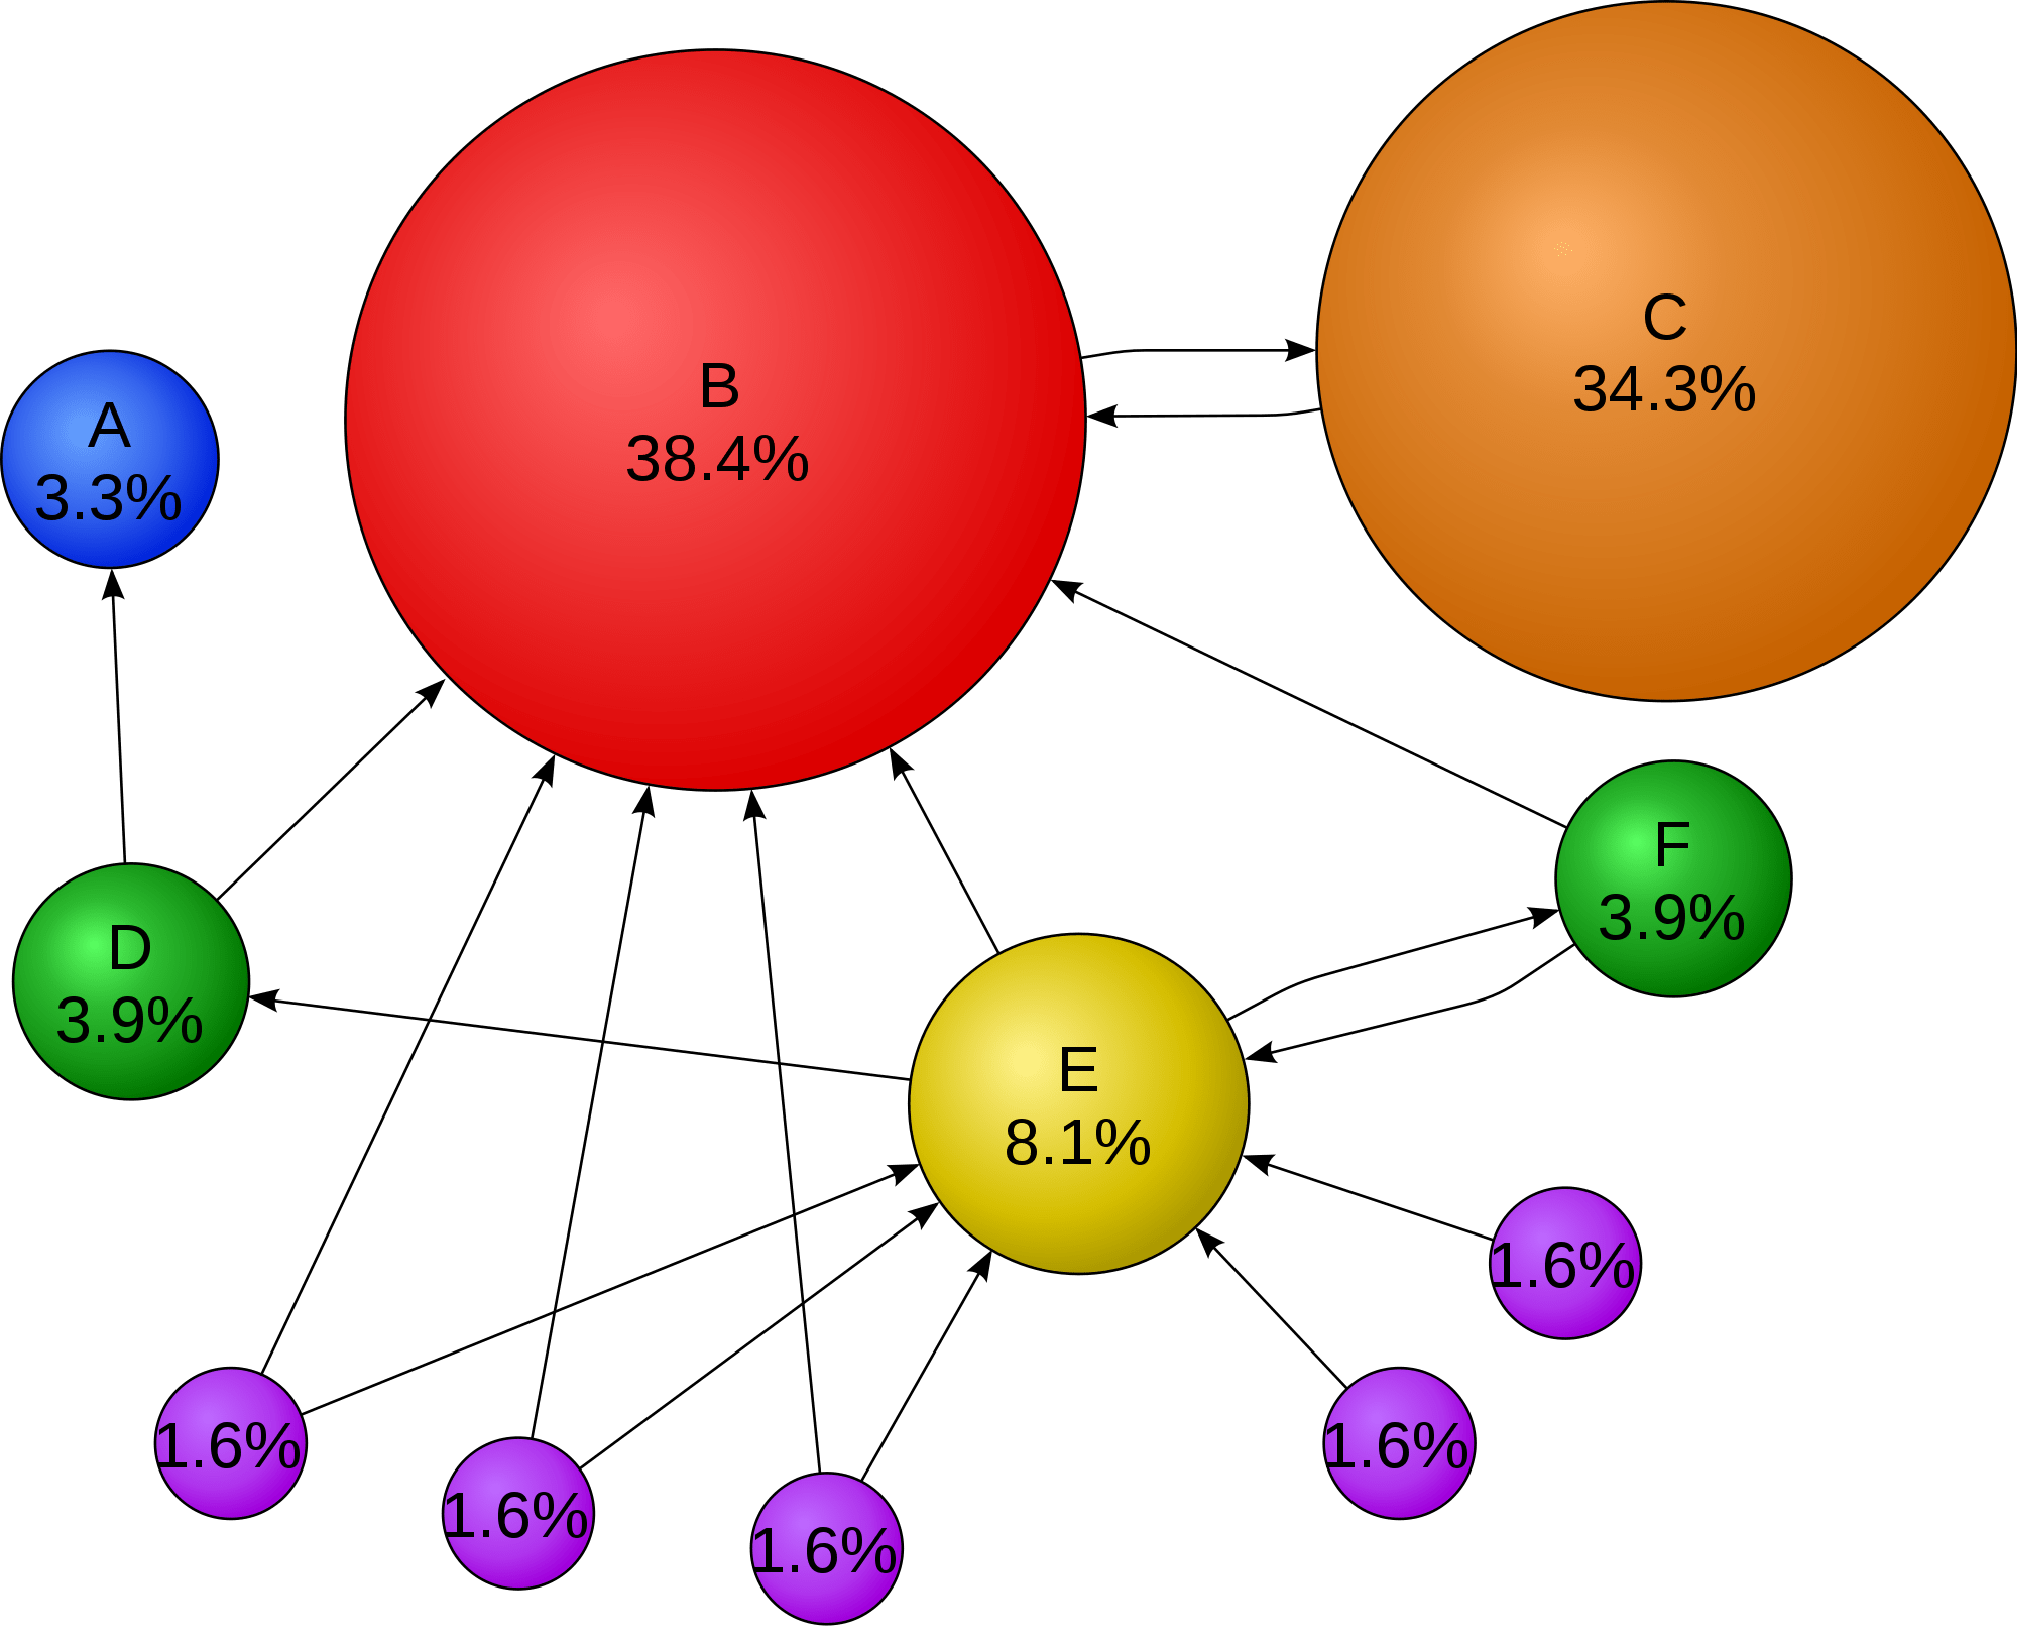
\includegraphics[width=\textwidth]{img/pagerank.png}
  \caption{Příklad ohodnocení PageRank algoritmem, zdroj: wikipedia.com}
  \label{fig:pagerank}
\end{figure}

Google přepočítává ohodnocení stránek \textbf{při každém crawlingu} (viz \ref{section:anatomy}). Se zvětšující se množinou stránek, které Google prochází a ohodnocuje, je ohodnocení jednotlivých stránek stále snižováno. Pokud se narazí na stránku, ze které nevedou žádné odkazy, PageRank algoritmus \textbf{rovnoměrně přerozdělí} ohodnocení této stránky na celou množinu jím hodnocených stránek (všechny stránky sítě WWW). Ve svém původním článku \cite{Page1998_2} autoři algoritmu uvádějí, že množina stránek obsahující 322 milionů odkazů konverguje k tolerovatelnému výsledku během 52 iterací. Množina poloviční velikosti pak konverguje po přibližně 45 iteracích. Skrze toto zjištění pak mohli autoři usoudit, že algoritmus je velmi dobře škálovatelný \cite{Page1998_2}.

Od zveřejnění PageRank algoritmu bylo objeveno několik black-hat SEO technik, které tohoto algoritmu zneužívají. Jednou z nich je například obchodování s umístěním odkazů na stránkách s vysokým ohodnocením, nebo např. vznik tzv. odkazových farem\footnote{\url{https://www.mattcutts.com/blog/how-to-report-paid-links/}}. Od prosince 2007 Google aktivně penalizuje takové počínaní - to jak odhaluje obchodování a odkazové farmy je firemním tajemstvím, je však známo, že se některé aktualizace algoritmů s označením Penguin a Panda zaměřují právě na potírání black-hat SEO technik.

\newpage
\textbf{Google Penguin algoritmus}
\label{section:penguin}

Google Penguin je označení pro aktualizaci vyhledávacích algoritmů vyhledávače Google, která byla poprvé oznámena 24. dubna 2012. Aktualizace se zaměřuje na \textbf{penalizaci} ohodnocení stránek, které porušují tzv. \textbf{Webmaster Guidelines\footnote{\url{https://support.google.com/webmasters/answer/35769?hl=en\#3}}} tím, že používají black-hat SEO techniky k manipulaci ohodnocení stránek skrze vytváření velkého množství odkazů směřujících na tyto stránky. Často se k tomu používá právě odkazových farem\footnote{\url{https://webmasters.googleblog.com/2012/04/another-step-to-reward-high-quality.html}}. Podle odhadů Penguin ovlivnil asi 3,1 \% vyhledávání v angličtině a přibližně 3 \% v jazycích jako němčina, čínstina, arabština a mnoho dalších vysoce zaspamovaných mutací WWW sítě. Google specificky zmiňuje tzv. \textbf{doorway pages}, které vydělávají pouze na tom, aby přilákaly publikum.\\

\textbf{Google Panda algoritmus}
\label{section:panda}

Google Panda je aktualizací vyhledávače Google představená v únoru 2011. Tato aktualizace se stejně jako Google Penguin (kapitola \ref{section:penguin}) zaměřuje na penalizaci spamových stránek a stránek s nekvalitním obsahem\footnote{\url{https://www.wired.com/2011/03/the-panda-that-hates-farms/}}. CNET po uvedení aktualizace zaznamenal pokles v ohodnocení zpravodajských a sociálních sítí a také pokles v oblasti stránek s velkým množstvím reklamy\footnote{\url{https://www.cnet.com/news/testing-googles-panda-algorithm-cnet-analysis/}}. Změna ovlivnila přibližně 12 \% všech vyhledávání\footnote{{\url{https://www.wired.com/2011/03/the-panda-that-hates-farms}}}.\\

\textbf{Knowledge Graph}
\label{section:knowledgegraph}

Knowledge graph je \textbf{strukturovaná databáze informací}, kterou Google začal používat v květnu 2012 (viz příloha \ref{app:GoogleUpdates}). Počáteční data byla převzata z databáze \textbf{Freebase}, \textbf{Wikipedia} a \textbf{CIA Fact Book} \cite{Enge2015}. Tato data uspokojila pouze malé množství dotazů a proto Google neustále svou databázi vylepšuje. Cílem je rychle zodpovědět základní dotazy zadané do vyhledávače. Na obrázku \ref{fig:knowledgegraph} můžeme vidět výsledek vyhledávání, na který byl knowledge graph použit. Výsledek poskytuje základní informace o VŠE - je nám poskytnuta mapa, logo, fotografie interiéru, popis, adresa, datum založení, telefon a další informace. Vše v přehledné tabulce na jednom místě.\\ 

\begin{figure}
  \centering
    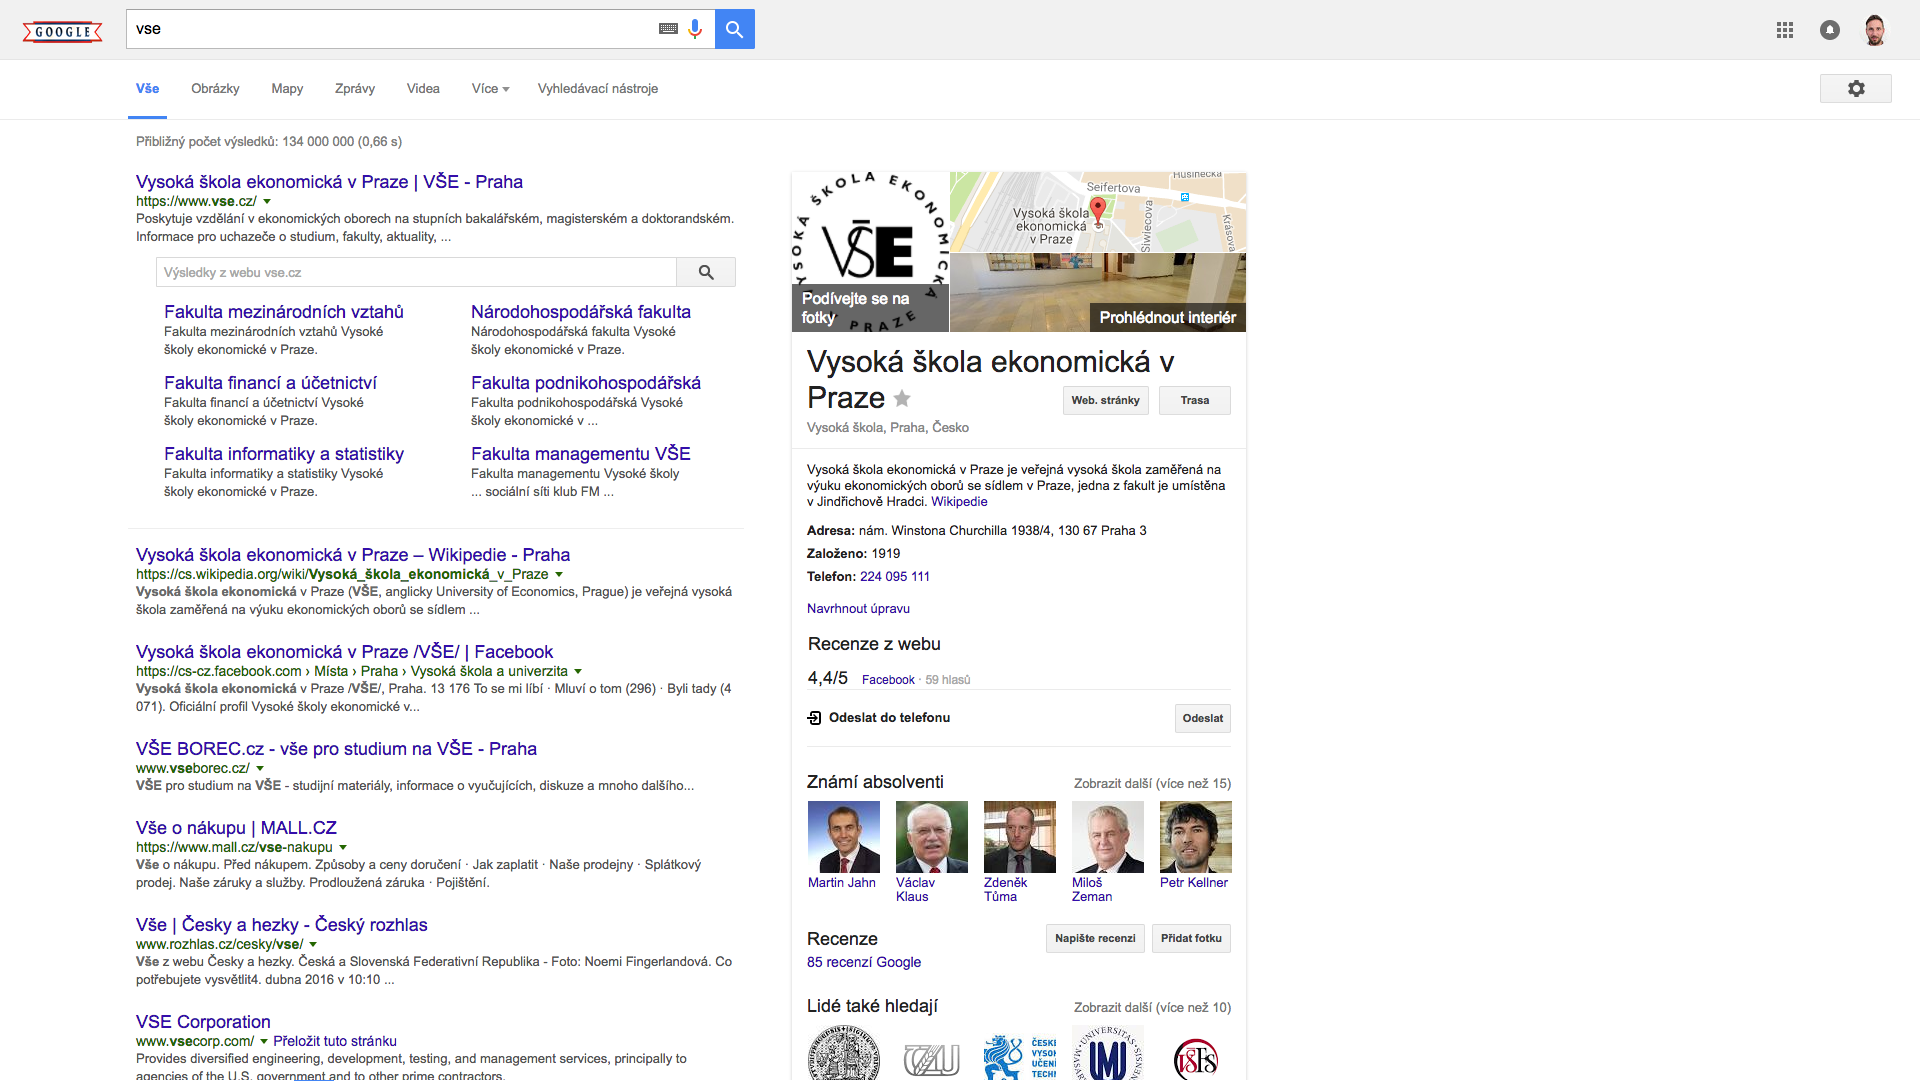
\includegraphics[width=\textwidth]{img/knowledgegraph.png}
  \caption{Ukázka použití knowledge graphu při vyhledávání, zdroj: google.com}
  \label{fig:knowledgegraph}
\end{figure}

\textbf{Analýza textu odkazu}\\
Dalším důležitým prvkem je samotný \textbf{text odkazu}. Tento text často obsahuje \textbf{klíčová slova}, která popisují web, na který se odkazuje. Tato klíčová slova pak pomocí sémantické analýzy vyhledávači vytvoří vcelku dobrou představu o obsahu odkazovaného odkazované stránky a celého webu.\\

\textbf{Signály sociálních sítí}\\
Weby jako \textbf{Facebook}, \textbf{Twitter} a \textbf{Google+} vytvořily zcela novou cestu ke sdílení a ohodnocení webů a jejich obsahu. Vyhledávače tyto informace používají a ohodnocují dle nich výsledky vyhledávaní. Dle článku respektovaného SEO portálu MOZ.com\footnote{\url{https://moz.com/blog/google-bing-confirm-twitter-facebook-influence-seo}} je možné vidět značnou korelaci mezi hodnocením pomocí tlačítka Google+1 a pořadím, ve kterém se vý\-sled\-ky zobrazují.\\

\textbf{Aktuálnost výsledků}\\
Většinou dává smysl upřednostňovat výsledky, které přečkaly tlak času a ospravedlnily svou existenci, někdy je však potřebné zobrazit \textbf{aktuální výsledky}. Při zemětřesení se například mnoho lidí začne vyhledávače vyptávat na informace, avšak první články se začnou objevovat až po 15 minutách. V těchto případech je potřeba indexovat nové články téměř v \textbf{reálném čase}. Google tento koncept označuje jako \textbf{Q}uery \textbf{D}eserves \textbf{F}reshness (\textbf{QDF}). Podle New York Times\footnote{\url{http://www.nytimes.com/2007/06/03/business/yourmoney/03google.html?_r=3&ref=yourmoney&pagewanted=all}} bere QDF v potaz několik faktorů:

\begin{itemize}
	\item Množství dotazů
	\item Množství zpráv
	\item Množství blogových příspěvků
\end{itemize}

QDF je aplikováno na výše popsaný příklad nebo také na nové produkty a slevy, na které je velké množství dotazů.   

\subsubsection{Negativní hodnotící signály}
Mimo pozitivních hodnotících faktorů, které jsme si uvedli výše, zkoumají vyhledávače také faktory, které mohou hodnocený web ovlivnit negativně \cite{Enge2015}.

\textbf{Jedná se např. o}:
\begin{itemize}
	\item \textbf{Malware} - Vyhledávače penalizují stránky, které obsahují viry a trojské koně.
	\item \textbf{Cloaking} - Penalizace za zobrazení jiného obsahu vyhledávači a jiného obsahu lidem.
	\item \textbf{Obchodování s odkazy} - Vyhledávače silně penalizují stránky, které obchodují s umístěním odkazů\footnote{\url{https://support.google.com/webmasters/answer/66356?hl=en&rd=1}}.
	\item \textbf{Rychlost stránek} - Roku 2010 Matt Cutts, vedoucí Google Web Spam oddělení, oznámil, že se rychlost stránek stala jedním ze signálů, které ovlivňují ohodnocení. Lidé, kteří neoptimalizovali obsah své stránky pro rychlé načítání tak získávají horší ohodnocení.\footnote{\url{https://www.mattcutts.com/blog/site-speed/}}
\end{itemize}


\subsubsection{Další hodnotící signály}
Jak bylo uvedeno v úvodu této kapitoly (\ref{section:signals}), hodnotících signálů je velké množství a stále přibývají. Uvedeme si ještě 2 důležité signály.

\begin{itemize}
	\item \textbf{Rychlost zisku odkazů} - Pokud vaše stránky získávají v průměru 5 odkazů za den a náhle začnou získávat 10 odkazů za den, vyhledávače budou na tuto změnu nahlížet jako na pozitivní signál. Pokud stránky z původních 5 odkazů získávají v průměru pouze 2 odkazy denně, jedná se naopak o negativní signál. Ve chvíli, kdy však stránky náhle začnou získávat 300 nových odkazů denně, jedná se buďto o silný nárůst publika, nebo o získávání odkazů pomocí spamu. Algoritmy se nejvíce zajímají o zdroj těchto odkazů a pokud se jedná o spam (viz kapitola \ref{section:blackhatseo}), budou stránky silně penalizovány. Koncept tohoto hodnotícího signálu je uveden v US patentu 20050071741\footnote{\url{http://appft1.uspto.gov/netacgi/nph-Parser?Sect1=PTO1&Sect2=HITOFF&d=PG01&p=1&u=/netahtml/PTO/srchnum.html&r=1&f=G&l=50&s1=\%2220050071741\%22.PGNR.&OS=DN/20050071741&RS=DN/20050071741}}.
	\item \textbf{Uživatelská data} - Vyhledávače berou také v potaz \textbf{lokaci vyhledávajícího}. To je velmi výhodné, pokud vyhledávající vyhledává například místní restauraci. Uživatel získá výsledky přizpůsobené místu, kde se aktuálně nachází a cesta k vyhledávané informaci se tak zkrátí. Dalším uživatelským faktorem je také \textbf{nastavení vyhledávače} - pokud uživatel preferuje výsledky v čestině, budou takovéto výsledky ohodnoceny lépe než např. více relevantní anglické výsledky. V neposlední řadě jsou tady také sinály z historie vyhledávání. 
	\item \textbf{Historie vyhledávání} - Jak jsme si ukázali (\ref{section:anatomy}), vyhledávací algoritmy jsou velice komplexní a často dokáží přesně odhadnout to, co uživatel dotazem zamýšlí. Problém však nastává v případě, kdy uživatel definuje svůj dotaz příliš obecně. Pokud například napíše \uv{auto}, vyhledávač neví, zda má uživateli poskytnout odkazy na nákup automobilu, na recenze automobilů, na autoškolu, nebo na něco jiného. Stejně tak tomu může být, pokud uživatel do vyhledávače napíše \uv{jaguar}. Vyhledávač sám o sobě neví, zda uživatel hledá automobil, nebo zvíře. Vyhledávače tento problém řeší pomocí adaptivního vyhledávání. Z historie vyhledávání jsou schopny určit pravděpodobný záměr aktuálního vyhledávání. Google tento koncept nazývá \textbf{Adaptive Search}. 
\end{itemize}

\newpage
\subsection{Shrnutí}
V části \ref{section:searchengines} jsme si ukázali jak se vyhledávače stali běžnou součástí našich životů, ukázali jsme jak pracují - jak sbírají informace o webových stránkách, jak tyto informace analyzují a na co se zaměřují. Koncepty vysvětlené v této kapitole jsou důležité pro pochopení SEO technik, které jsou popsány v kapitole \ref{section:SEO} a při aplikaci technik v praktické části. Nyní se přesuneme k dalšímu subjektu, kterého se vyhledávání týká - uživatel. 


\newpage
\section{Lidé a vyhledávače}
\label{section:howpeoplesearch}
Vyhledávače investují velké množství svých zdrojů do výzkumu toho, jak lidé s vyhledávačem zacházejí. To jim umožňuje podávat lepší (rychlejší, čerstvější a relevantnější) výsledky. Poznatky z výzkumu a jejich implementace podněcují vytváření čitelných a použitelných webů, jelikož kompatibita s vyhledávači přináší pozitiva v podobě lepšího ohodnocení a umístění ve výsledcích \cite{Enge2015}.

V této části práce bude ukázáno, \textbf{jak uživatelé s vyhledávačem interagují} - to je oblast studia pro vyhledávače i SEO. Vyhledávače se přizpůsobují uživatelům a SEO se přizpůsobuje aktuálním vyhledávačům, pro které optimalizuje webové stránky z důvodu potencionálních vyšších zisků. Ukážeme si jak roste celý sektor vyhledávání a SEO a také to, jak se mění vyhledávací strategie uživatelů. 

\subsection{Vyhledávací strategie}
\label{section:searchstrategy}

\subsubsection{Cíle vyhledávání}
Základním cílem vyhledávání je získání informací popsaných \textbf{vyhledávacím dotazem} v podobě množiny klíčových slov a frází vložených do vyhledávacího pole. Uživatel ho může formulovat jako \textbf{otázku}, avšak většina dotazů je jednoduše formulována jako \textbf{kombinace klíčových slov}. Vyhledávače se v průběhu let značně vyvinuly, avšak primární principy vyhledávání zůstávají nezměněny.

\begin{itemize}
	\item Uživatelé pociťují potřebu po informaci. 
	\begin{itemize}
		\item Mohou hledat informaci obsaženou na specifické webové stránce, nebo webovou stránku samotnou (\textbf{navigační dotaz})
		\item Mohou chtít něco koupit (\textbf{transakční dotaz})
		\item Mohou se chtít něco naučit (\textbf{informační dotaz})
	\end{itemize}
	\item Uživatel formuluje dotaz pomocí klíčových slov a frází
	\item Uživatel odešle dotaz a zkontroluje výsledky
\end{itemize}

Výzkum z Pennsylvania State University a z Queensland University of Technology ukazuje, že více než \textbf{80 \% dotazů je informačního charakteru} a pouze kolem \textbf{10 \% je transakčního, nebo navigačního typu} \cite{Jansen2008}.

\subsubsection{Způsob vyhledávání}

\textbf{Interakce uživatele s vyhledávačem může být vícekrokovým procesem}. Na obrázku \ref{fig:merrellshoes} můžeme vidět ukázku vyhledávání bot. Uživatel hledá boty značky Merrell. Začne na internetovém obchodu \texttt{www.onlinestores} a pokračuje na oficiální stránku této značky. Zřejmě se uživateli boty líbí, hledá slevu na tyto boty, pak specifikuje dotaz a hledá dámské sandály této značky a přechází na web \texttt{www.coachlikeapro.com}. Tam uživatele pravděpodobně zaujmou boty značky Clarks, které po dvou dotazech konečně zakoupí v internetovém obchodu \texttt{www.easyspirit.com}. Finální rozhodnutí padne až po 55 minutách a 44 sekundách.

\begin{figure}
  \centering
    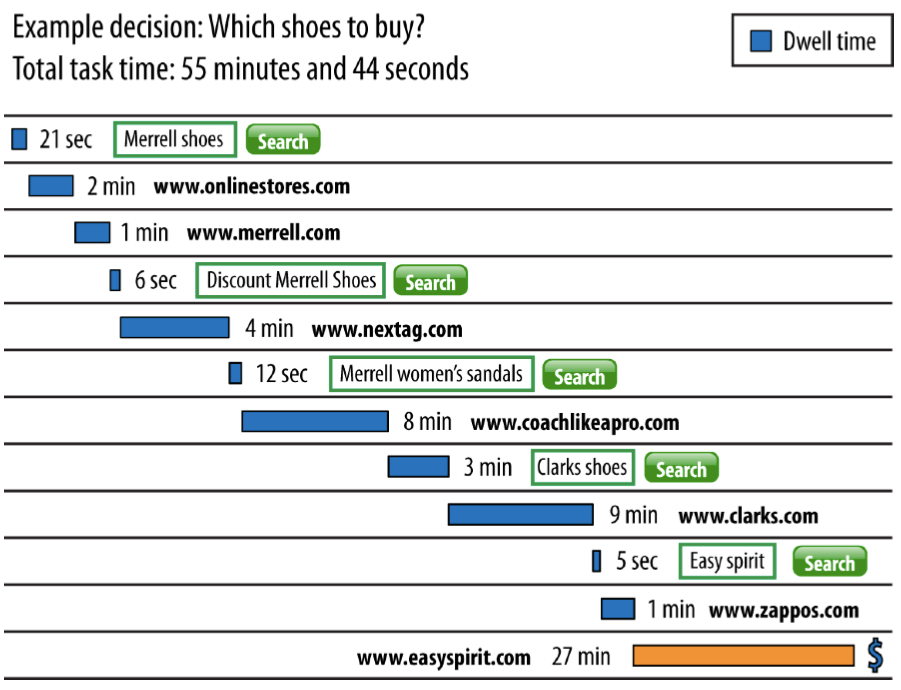
\includegraphics[width=\textwidth]{img/merrellshoes.png}
  \caption{Ukázka postupu vyhledávání bot, zdroj: \cite{Enge2015}}
  \label{fig:merrellshoes}
\end{figure}

\begin{table}
\centering
\begin{tabular}{|l|l|}
  \hline
  \textbf{Interval mezi prvním návštěvou a nákupem} & \textbf{Procento uživatelů} \\
  \hline
  Stejný den & 50 \% \\
  \hline
  2-7 dní & 9 \% \\
  \hline
  8-30 dní & 12 \% \\
  \hline
  31-90 dní & 26 \% \\
  \hline
  Více než 90 dní & 3 \% \\
  \hline
\end{tabular}
\caption{Tabulka zobrazující interval mezi první návštěvou a nákupem, zdroj: \cite{Enge2015}}
\label{tab:interval}
\end{table}

Tabulka \ref{tab:interval} ukazuje pravděpodobnost koupě (konverze) po určitém čase započatém prvním příchodem zákazníka. Lidé vybírají v několika krocích - obecně se může jednat o hledání nejnižší ceny, nebo může jít např. o vyhledávání důvěryhodnějšího prodejce.

\begin{figure}
  \centering
    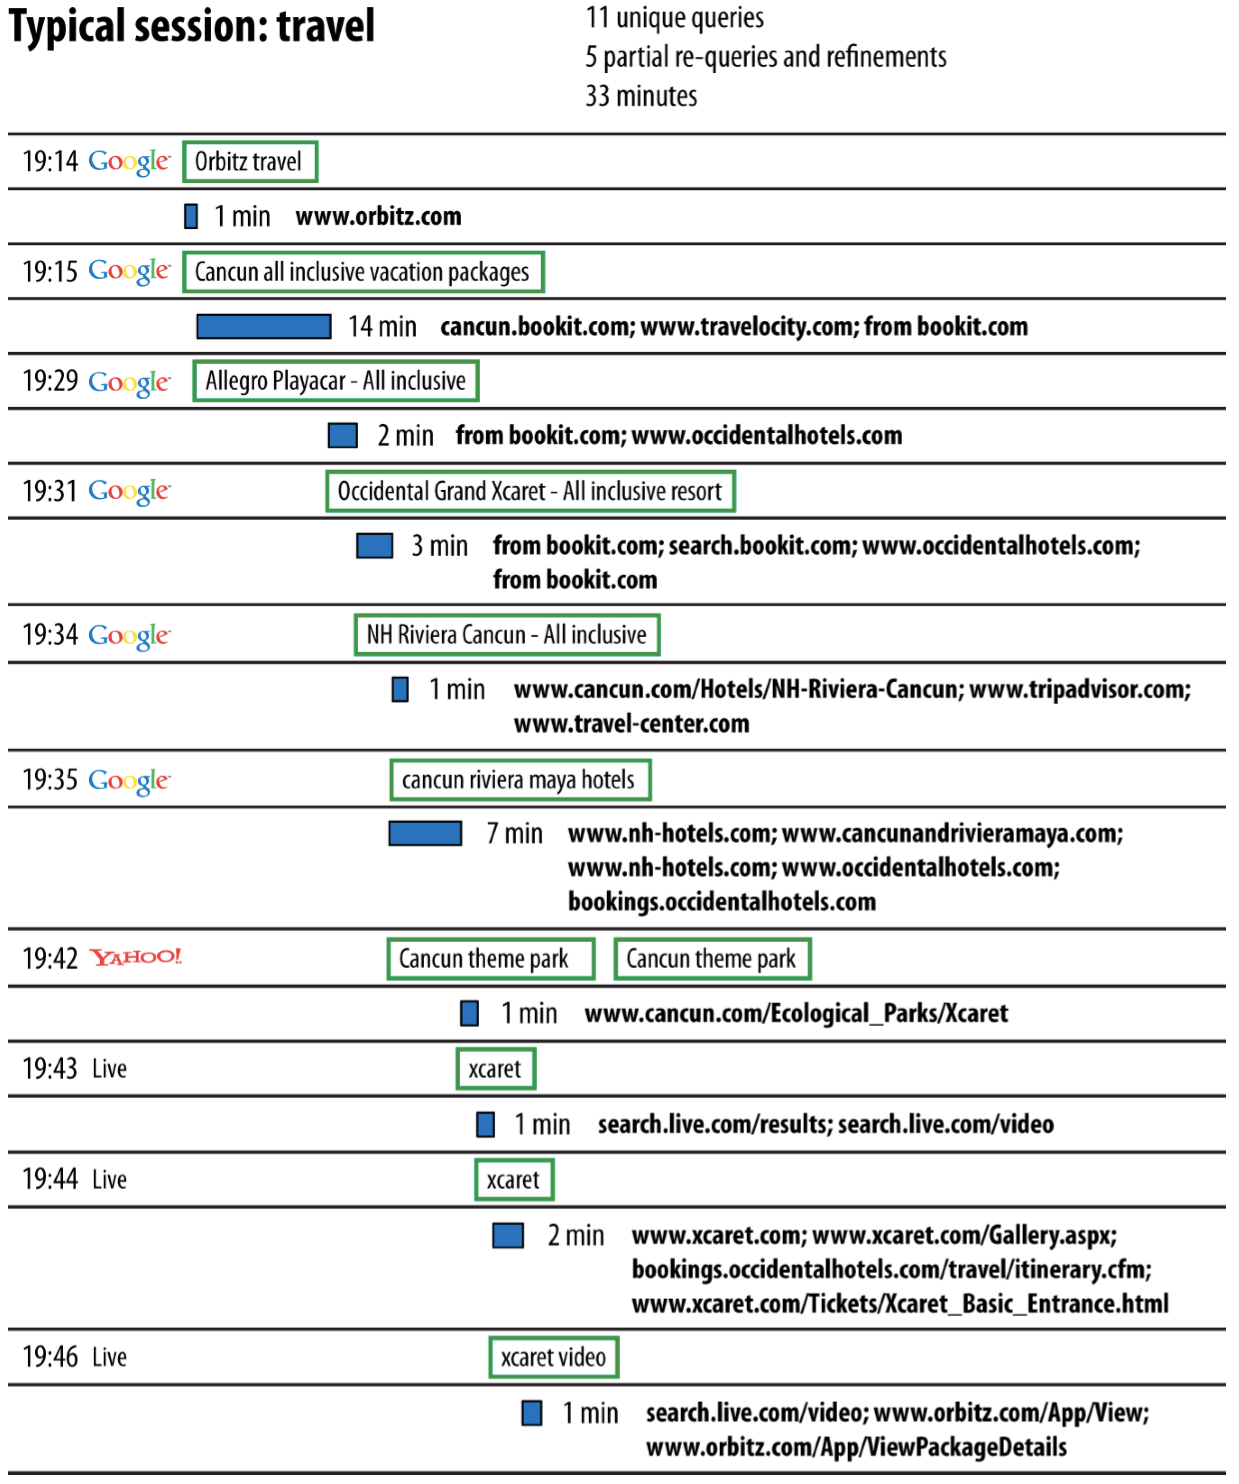
\includegraphics[width=\textwidth]{img/orbitz.png}
  \caption{Ukázka vyhledávání ubytování, zdroj: \cite{Enge2015}}
  \label{fig:orbitz}
\end{figure}

Další příklad vyhledávání je na obrázku \ref{fig:orbitz}. Uživatel chce jednoduše najít cestovatelskou webovou stránku \texttt{www.orbitz.com}. Uživatel na této stránce zůstane pouze 1 minutu a pak začne hledat \uv{Cancum all inclusive vacation packages} - all inclusive ubytování v oblasti Cancum. Následuje vyhledávání několika specifických resortů a konečně se rozhodne pro Cancum Riviera Maya Hotels a zabookuje si ubytování na \texttt{bookings.occidentalhotels.com}. Uživatel následně vyhledává možnosti kulturního vyžití - změní vyhledávání na \uv{cancum theme park} a následně začne hledat informace o \uv{xcaret}, velmi známém ekoparku poblíž ubytování. \textbf{Uživatelé často mění strategie vyhledávání, aby našli požadovanou informaci}. Příklady na obrázku \ref{fig:merrellshoes} a \ref{fig:orbitz} jsou typickými příklady vyhledávání. Nedávná data také ukazují, že se \textbf{uživatelé chovají jiným způsobem ve chvíli, kdy vyhledávají na mobilním zařízení}. Vyhledávače se přizpůsobují tomuto způsobu vyhledávání a volbě různých vyhledávacích strategií. Z těchto důvodů musí SEO specialista rozumět lidskému záměru vyhledávání také.

\subsubsection{Přesun k mobilním zařízením}
\label{section:mobileshift}
V březnu 2015 server eMarketer\footnote{\url{https://www.emarketer.com}} publikoval studii ukazující růst reklamy v mobilním segmentu na úkor reklamy na desktopu. Předpokládá se, že do roku 2019 vzrostou výdaje na mobilní reklamu na \textbf{65.87 billionů dolarů, což je 72.2 \% celkových výdajů za reklamu v US}. Růst je možné vidět na obrázku \ref{fig:deviceadspending}.
Podle výzkumu analytického serveru StatCounter stoupl v listopadu 2016 počet přístupů z mobilních zařízení natolik, že překonal klasické desktopy (stolní počítače a notebooky)\footnote{\url{http://gs.statcounter.com/press/mobile-and-tablet-internet-usage-exceeds-desktop-for-first-time-worldwide}}.

\begin{figure}
  \centering
    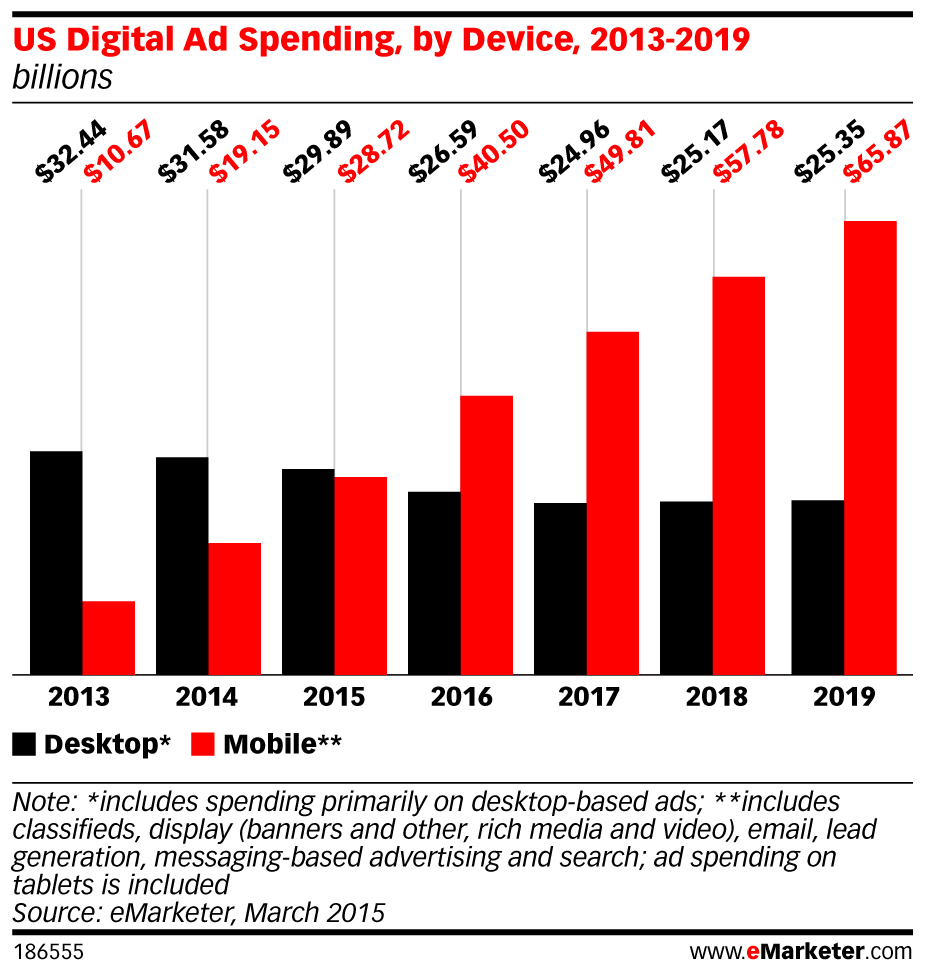
\includegraphics[width=\textwidth]{img/deviceadspending.png}
  \caption{Porovnání trhů digitalní reklamy na destopech a mobilních zařízeních, zdroj: eMarketer.com}
  \label{fig:deviceadspending}
\end{figure}

V souvislosti s růstem mobilního sektoru vyhledávání je nutno zmínit, že uživatelé na mobilních zařízeních používají jiné vyhledávací strategie. Dle studie společnosti Forrester\footnote{\url{http://blogs.forrester.com/julie_ask/16-07-26-mobile_search_its_different}} se mobilní strategie vyhledávání liší hlavně v těchto bodech:

\begin{itemize}
	\item \textbf{Lokalizace uživatele} - S příchodem mobilních zařízení bylo uživateli umožněno získávat informace kdykoliv a kdekoliv. Uživatelé přechází od plánování k akci - často věci spontánně řeši na poslední chvíli. Mobilní zařízení jsou běžně používané na vyhledávání restaurací, obchodů či autobusových zastávek v okolí místa, kde se uživatel aktuálně nachází. 
	\item \textbf{Rychlost} - Uživatel mobilního zařízení vyhledává, aby mohl ihned vyhledané informace uplatnit, nebo ihned koupit produkt, který našel. Uživatelé jsou dnes často závislí na svém mobilním zařízení a vyhledávání typu \uv{doprava z letiště do hotelu Hilton} jsou běžně prováděny až na letištích bez předchozího plánování. 
	\item \textbf{Bohatý obsah} - Mobilní stránky byly dříve používány k prezentaci základních informací - telefoního čísla uživatelské podpory, adresa, atd. Dnes jsou mobilní stránky komplexní a mají buďto stejnou, nebo velmi podobnou funkcionalitu jako jejich desktopové verze. 
	\item \textbf{Komplexní vyhledávání} - Komplexní vyhledávání je stále výsadou desktopových zařízení.
\end{itemize}

\subsection{Čtení výsledků}
V roce 2006 byla založena společnost Enquiro (dnes Mediative), která provedla testování \textbf{zaměření pozornosti vyhledávajcích uživatelů}. Výsledek je vidět na heat-mapě na obrázku \ref{fig:googleheatmap}. Je vidět, že uživatel se zaměřuje podstatně více na první 4 výsledky než na výsledky ostatní. První výsledek získává 18,2 \% prokliků, druhý výsledek 10,1 \%, třetí 7,2 \% a čtvrtý už pouze 4,8 \%. Studie \cite{usageresearch} a \cite{usageresearch2} ukazují podobné rozdělení a také to, jak je důležité držet se na předních místech ve výsledcích vyhledávání.

Přístup k vyhledávání se změnil při uvedení \textbf{Google Universal Search}, který zobrazuje deset vybraných relevantních webů (\uv{10 blue links}) a přidává obrázky, video, zprávy a další relevantní výsledky různých datových typů. Další vyhledávače postupně začaly používat stejnou techniku a dnes je tento přístup obecně nazýván blended search (více v kapitole \ref{section:searchui}). Způsob vyhledávání typu \uv{blended search} je na obrázku \ref{fig:googleheatmapblended}. Je možné vidět, jak se pozornost uživatele rozdělila mezi výsledky různých datových typů. Tento způsob vyhledávání je člověku bližší, jelikož spojuje typy informací dle kontextu a připomíná tak lidskou asociativní paměť (více v kapitole \ref{section:searchui}). 

\begin{figure}
  \centering
    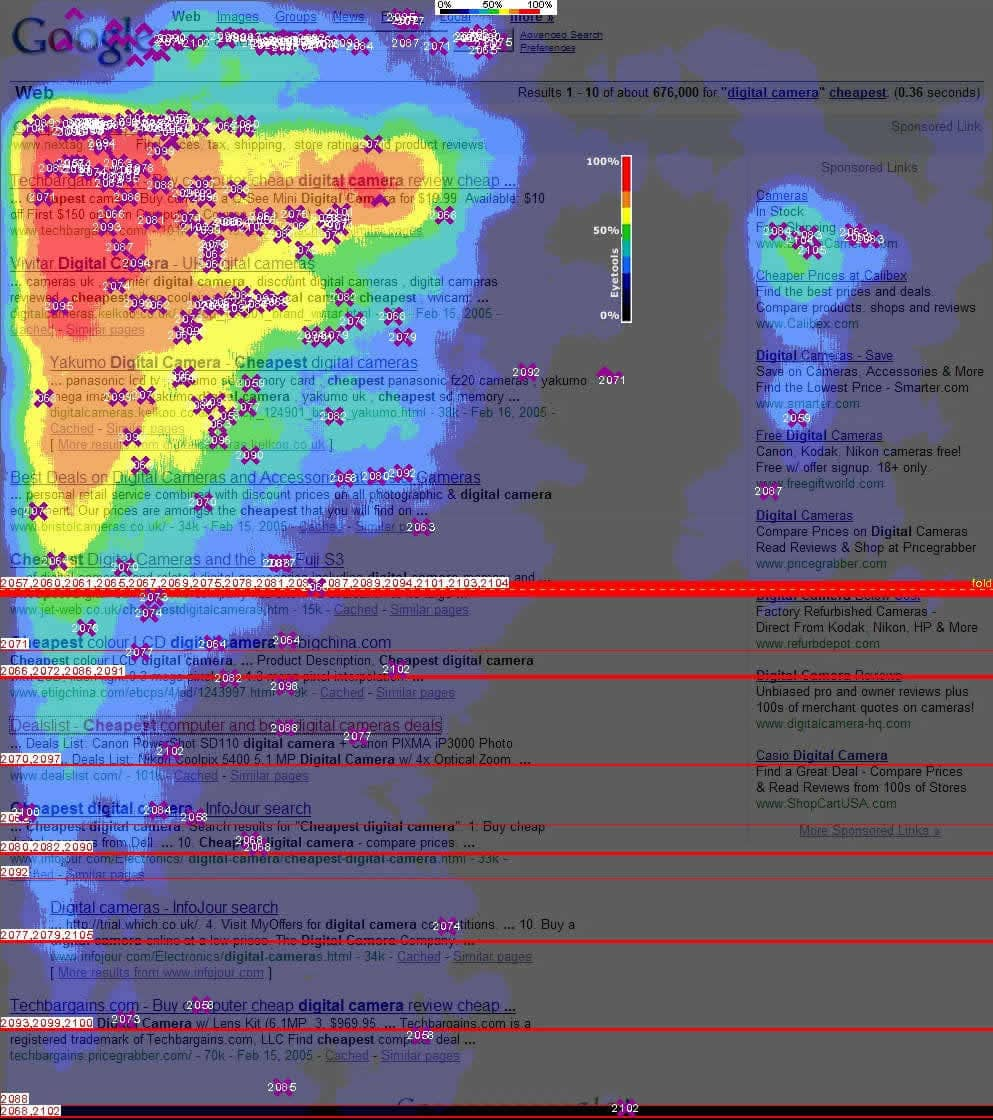
\includegraphics[width=\textwidth]{img/googleheatmap.jpg}
  \caption{Výsledky eye-tracking studie na Google.com, zdroj: Enquiro}
  \label{fig:googleheatmap}
\end{figure}


\begin{figure}
  \centering
    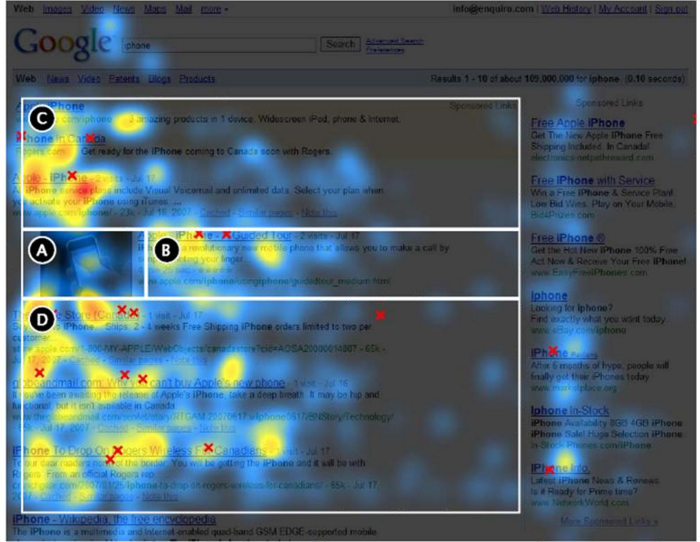
\includegraphics[width=\textwidth]{img/googleheatmapblended.png}
  \caption{Výsledky eye-tracking studie na google.com, \uv{blended search}, zdroj: Enquiro}
  \label{fig:googleheatmapblended}
\end{figure}

\subsection{Vliv vyhledávačů na společnost}
\label{section:society}
Vzhledem k tomu, že uživatelé z velké části využívají k přístupu do sítě WWW vyhledávače, jsou ovlivněny tím, jaké výsledky jsou jim poskytovány. \textbf{Laura Granka} se zabývá tím, \textbf{jak lidé vnímají výsledky vyhledávání a jak výsledkům na prvním pozicích dávají svou důvěru}. PageRank algoritmus (kapitola \ref{section:pagerank}) se spolu s dalšími signály stává hodnotícím faktorem produktů, ruzných druhů podnikání a celkové kvality informací na WWW. Informace, které uživatel vnímá jsou primárně ty, které jsou na prvním pozicích. Ty pak následně \textbf{utvářejí jeho pohled na svět}. Je důležité si uvědomit, že informace jsou nám předkládany na základě výsledků algoritmů, které nemají stejný kognitivní systém jako lidé a poskytnutá informace tak nemusí být vybrána vhodně \cite{Granka2010}.

\label{section:attentioneconomy}
\textbf{Matteo Pasquinelli} hledá spojitosti mezi PageRank algoritmem a myšlenkou \textbf{ekonomie pozornosti}\footnote{\url{https://en.wikipedia.org/wiki/Attention_economy}}. V ekonomii pozornosti je hodnota přiřazena produktu, který získává širší pozornost a tím pádem získává také lepší PageRank ohodnocení (více referencí - odkazů). Díky lepšímu ohodnocení je častěji zobrazován mezi nejlepšími výsledky vyhledávání, vstupuje do lidského vědomí v širším měřítku a může tak pravděpodobněji ovlivnit lidské rozhodování a akce. Díky lepší pozici ve vyhledávání je zaručena vyšší návštěvnost a tím pádem i více nákupů. \textbf{PageRank tak určuje důvěryhodnost, která ovliňuje naše akce} \cite{KonradBecker2009}.

\textbf{Katya Mayer} na PageRank nahlíží jako na způsob, kterým jsou \textbf{různé pohledy a my\-šlen\-ky sdružovány na jednom místě}. Lidé vyhledávající informace skrze vyhledávač (a tím pádem i PageRank algoritmus či jeho obdobu) jsou zaplaveni citacemi autorů, kteří mají na dané téma také nějaký názor. Tím je vytvořeno místo, kde může být vše diskutováno a shromažďováno. Toto místo se neustále adaptuje a stává se tak bodem, který \textbf{umožňuje hloubkový sociometrický průzkum na aktuálních datech} \cite{KonradBecker2009}.

\subsection{Shrnutí}

V této části jsme si ukázali jakým způsobem uživatel interaguje s vyhledávačem a jak může měnit strategie k nalezení požadovaných informací. Pochopení toho, jak uživatel vyhledává námi poskytovanou informaci je zásadním krokem pro návrh a implementaci SEO. Jsme pak schopni přizpůsobit klíčová slova tak, aby odpovídali vyhledácím dotazům. Nejde však pouze o to. Jde o vytvoření kvalitního \uv{internetového profilu}, který svědčí o kvalitě a důvěryhodnosti poskytovaných informací a také o celkovou komunikaci s klientem, kvalitu nabízených služeb, hodnotu a stabilitu značky či dostatek kvalitních hodnocení. 

V kapitole \ref{section:society} bylo diskutováno zpětné působení výsledků algoritmů na člověka. Výsledky, které jsou člověku často předkládány jsou posilovány pozitivní zpětnou vazbou. Více se o nich mluví, je na ně více referencí a udržují si svou pozici. Pro úspěch musí být marketingová strategie použita i v offline prostředí - musí se člověku udržovat v paměti i v prostoru kolem něj.

V praktické části si ukážeme rozšíření SEO optimalizace o propagaci na sociálních sítích. Vzhledem k tomu, že obsah sociálních sítí je vytvářen lidmi kolem nich, jsou sociální sítě kanálem s vysokým dosahem. 

\newpage
\section{SEO}
\label{section:SEO}

SEO, neboli \textbf{S}earch \textbf{E}ngine \textbf{O}ptimalization je \textbf{informatická a marketingová disciplína}, která se soustředí na publikaci informací ve formátu, který webové vyhledávače dokáží dobře rozpoznat a přibližuje tak uživatelům informace skrze lepší viditelnost ve výsledcích vyhledávání. Ve svých počátcích se SEO zaměřovalo na optimalizaci názvů souborů, titulků stránek a jejich metadata. S rozvojem vyhledávačů a se změnou jejich algoritmů se optimalizace stávala stále komplexnější. Do konce roku 2003 bylo velice jednoduché optimalizovat - stačilo koupit několik silných pozic pro umístění zpětného odkazu na dobře ohodnocených doménách. Po roce 2003 začal Google nasazovat sémantické hodnocení obsahu a začal penalizovat stránky zneužívající mezer vyhledávacích algoritmů. Pořadí ve výsledcích doznalo prudkých změn (viz aktualizace algoritmů v příloze \ref{app:GoogleUpdates} a kapitola \ref{section:anatomy}). V posledních letech se SEO stalo \textbf{jednou z hlavních součástí digitálního marketingu}. Hlavní příčinou rozvoje tohoto odvětví se stala skutečnost popisovaná ve statistikách o chování uživatelů na webu (kapitola \ref{section:howpeoplesearch}) - \textbf{jsou-li lidé online, vyhledávají}. 

Investice do SEO zvyšuje zisky online bussinessu a pro úspěch v konkurenčním boji je dnes taková investice nutná. Stejně tak, jak je tomu v ostatních makretingových oborech, je SEO \textbf{iterativním procesem}, který vyžaduje neustálé sledování vývoje aktuálních vyhledávacích a webových technologií a aplikaci nově nabytých poznatků. Výsledky SEO nemají okamžitou zpětnou vazbu a je tedy nutné dlouhodobé sledování různých faktorů, aby se dané webové stránky udrželi na nejlepším možném místě ve výsledcích vyhledávání. Google často své algoritmy mění a pro SEO při těchto změnách začíná tzv. \textbf{\uv{Google Dance}}\footnote{\url{https://metamend.com/archive/education/google-dance/}} - postupná reoptimalizace vůči změnám algoritmů.

 Společnosti v roce 2015 za služby SEO utratily \textbf{65 billionů dolarů} a tento sektor neustále roste. Je to trojnásobek toho, co bylo předpovězeno v roce 2008\footnote{\url{http://www.mediapost.com/publications/article/273956/report-companies-will-spend-65-billion-on-seo-in.html}}. Na obrázku \ref{fig:channelsfig} je možné vidět provázanost SEO s ostatními marketingovými oblastmi. Vyhledávání je v samotném průsečíku sektorů prodeje, brandingu (budování značky) a online marketingu. Vyhledávač má širokého využití. Může se jednat o průzkum, lokalizaci či koupi produktů. Tržby eCommerce neustále stoupají (obrázek \ref{fig:forrester}), \textbf{pro rok 2017 je odhadováno 370 billionů USD}, což je 10 \% veškerého koncového prodeje. Růst tohoto sektoru podporuje růst sektoru SEO. Tyto dva sektory se vzájemně posilují a během posledních let změnily způsob, kterým nakupujeme. 

V této části práce si ukážeme výhody SEO, jeho stručnou historii, ukážeme si, jaké prvky ovlivňují SEO strategii a v neposlední řadě si ukážeme některé z white-hat a black-hat SEO technik, které budeme používat v praktické části. 

\begin{figure}
  \centering
    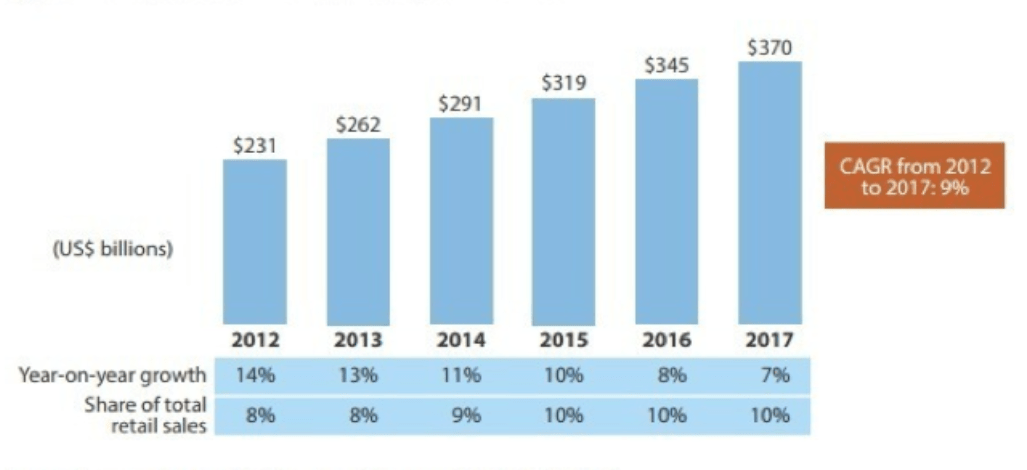
\includegraphics[width=\textwidth]{img/forrester2017.png}
  \caption{Předpověď online prodejů pro rok 2017, zdroj: Forrester Research, Inc.}
  \label{fig:forrester}
\end{figure}

\begin{figure}
  \centering
    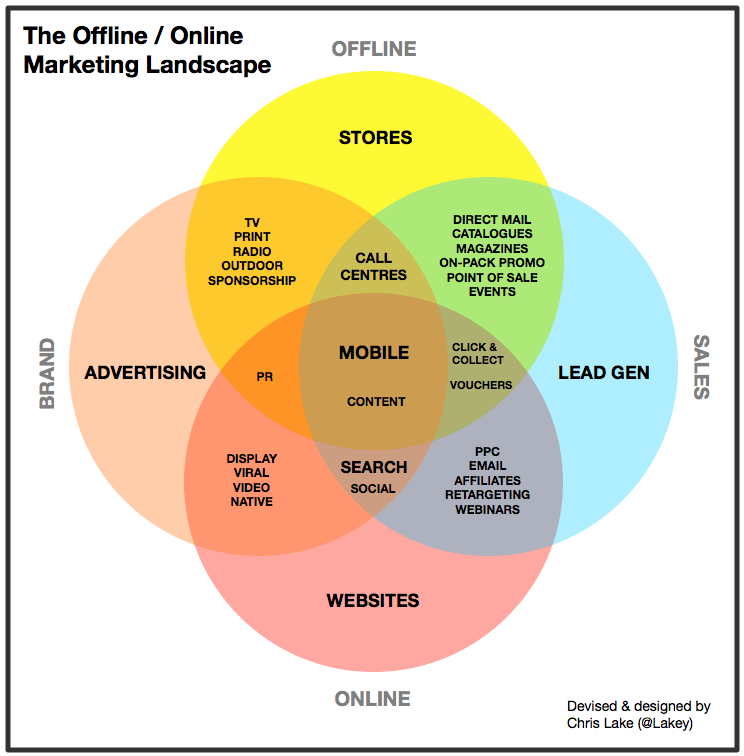
\includegraphics[width=\textwidth]{img/channelsfig.png}
  \caption{Vyhledávání v širších marketingových souvislostech, zdroj: Econsultancy}
  \label{fig:channelsfig}
\end{figure}

\newpage
\subsection{Výhody SEO}
\label{section:seoplus}
\subsubsection{Viditelnost (Branding)}

Branding je komplex úkonů, které vedou k vybudování úspěšné značky. Jde například o vytvoření trefného názvu, loga, sloganů a všeho, co posiluje povědomí dané značky u svých zákazníků. Značka může představovat samotného výrobce zboží, avšak většinou je něčím více - dalo by se říci, že značka je vytvářena jako určitá forma komunikace s koncovými zákazníky. Značka je také abstraktní strukturou, do které její tvůrci vkládají hodnoty, se kterými se její zákazníci mohou ztotožnit. Mnoho uživatelů webových vyhledávačů chápe umístění ve vyhledávači také jako součást značky. Čím výšší je postavení ve vyhledávání, tím větší kvalita se očekává - cílem vyhledávacích algoritmů je také poskytnout nejvíce relevantní informace k danému vyhledávanému řetězci. Zisk dobrého umístění zvyšuje sílu značky a SEO je tedy součástí brandingu. Podle statistik z roku 2015\footnote{\url{http://interbrand.com/best-brands/best-global-brands/2015/ranking/\#?listFormat=ls}} patří mezi nejúspěšnější globální značky Apple, Google, Coca Cola, Microsoft a IBM. 

\subsubsection{Zvýšení návštěvnosti}

Posunem na vyšší pozice ve vyhledávání zaznamenávají stránky exponenciální nárůst návštěv\-nos\-ti. Jak bylo uvedeno v kapitole \ref{section:howpeoplesearch}, první 4 odkazy získávají velké procento celkové návštěvnosti. První výsledek získává 18,2 \% prokliků, druhý výsledek 10,1 \% prokliků, třetí 7,2 \% prokliků a čtvrtý už pouze 4,8 \% prokliků. K dosažení takto kvalitních výsledků U těchto výsledků však samotné SEO nestačí a je potřeba nasadit \textbf{komplexní marketingový plán}. Takový plán se vyznačuje svým iterativním vylepšováním - nestačí jednou optimalizovat, aby bylo vše hotovo, protože \textbf{hotovo nikdy není}. Způsob, jakým lidé vyhledávají, se mění a s tím se mění také klíčová slova, která jsou při vyhledávání používána. Jedním z úkolů SEO profesionála je \textbf{průzkum klíčových slov}, na které se při optimalizaci zaměřit. Pokud se například vyhledávající zajímá o \uv{hybridní úsporný automobil}, je vysoce pravděpobné, že se právě na takovouto kombinaci klíčových slov zaměří výrobce elektromobilů a to i v případě, že se kombinace klíčových slov \uv{elektromobil} nebo \uv{elektrický automobil} v dotazu \uv{hybridní úsporný automobil} nevyskytuje. 

\subsubsection{Vysoká návratnost investice}

Zvýšení viditelnosti a návštěvnosti je pouze prvním krokem k úspěchu. Cesta k úspěchu opět vede skrze iterativní proces vyhodnocování a postupného zlepšování SEO strategie tak, \textbf{aby bylo dosaženo cíle}. Pro někoho může být cílem jeho strategie zvýšení \textbf{tržeb}, pro někoho jiného to však může být předání nějaké \textbf{vize}. Nelze tedy pokaždé použít stejný SEO přístup, vždy je nutné SEO \textbf{přizpůsobit} dáné strategii a cíli.
Samotná návštěvnost také nezaručuje úspěch. \textbf{Jde primárně o návštěvníky, kteří jsou schopni vykonat akci} související s naším cílem - koupit si produkt, nebo např. šířit dál naši myšlenku. Takové akci se v odvětví SEO říká \textbf{konverze}. Dobře navržená SEO strategie má potenciál velké návratnosti (viz Attention Economy Matteo Pasquinelliho - \ref{section:attentioneconomy}). SEO obecně přináší \textbf{vyšší návratnost než televizní/radio reklamy}. Stejně tak tomu je v porovnání s reklamnímy letáky. Důvod lze hledat hlavně v \textbf{přesunu pozornosti od těchto médií k internetu}. Mnoho dnešních businessů se soustředí čistě na prostředí internetu a ostatní média budťo nevyužívají vůbec, nebo pouze ve velmi omezené míře. Příkladem může být LindedIn, Amazon, nebo eBay. Pro online business je důležité udržet se v předních výsledcích vyhledávání a proto je SEO v takovém rozkvětu. 
Podle studie ze srpna 2016\footnote{\url{https://econsultancy.com/blog/67734-three-key-charts-from-our-2016-email-marketing-census/}} je SEO v návratnosti investice hned za e-mailem, který 73 \% respondentů označilo za excelentní nebo dobrý kanál v návratnosti investice. SEO samotné je na druhé příčce s 67 procenty (obrázek \ref{fig:channels}). 

\begin{figure}
  \centering
    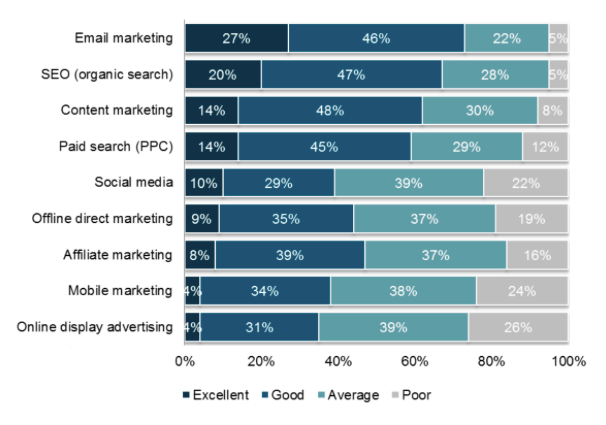
\includegraphics[width=\textwidth]{img/channels.png}
  \caption{Porovnání návratnosti investice, zdroj: Econsultancy}
  \label{fig:channels}
\end{figure} 

\subsection{Stručná historie SEO}

V následujících několika odstavcích si ve stručnosti představíme historii vývoje SEO. K porozumění souvislostí doporučuji procházet až po přečtení kapitoly \ref{section:searchenginehistory}.

Webmasteři se o optimalizaci svých stránek pro webové vyhledávače začali zajímat v polovině 90. let, v době kdy se rozmáhala nová technologie World Wide Webu a kdy vznikaly první vyhledávače, které analyzovaly webové stránky. Z počátku stačilo odeslat URL adresu do vyhledávače, vyhledávací robot naindexoval stránky a stránka se zobrazila ve výsledcích vyhledávání. Vlastníci webových stránek si při pohledu na úspěch své konkurence začaly uvědomovat důležitost dobrého umístění ve vyhledávačích a otvíraly se tak dveře pro white-hat i black-hat SEO specialisty. 

Vyhledávací algoritmy tehdejších vyhledávačů spoléhaly na analýzu názvů souborů a na klíčová slova uvedená v \texttt{<meta name='keywords'>} v \texttt{<meta name='description'>} HTML tagu, který měl sloužit k popisu stránek. Ukázalo se však, že do \texttt{<meta>} tagu se často uvádí nepřesný popis a to znemožnilo vyhledávači doručit jeho uživateli relevantní výsledky \cite{Doctorow2001}. Tento HTML tag byl také zneužíván k tzv. \uv{keyword stuffingu} (viz kapitola \ref{section:keywordstuffing}) a bylo s ním možné manipulovat s výsledky vyhledávání. Roku 1997 postupně vyhledáče (AltaVista, Infoseek - viz \ref{section:searchenginehistory}) od analýzy tohoto tagu postupně upustilo a namísto hustoty klíčových slov začaly vyhledávače raději zkoumat samotný sémantický obsah webových stránek \cite{Flynn1996}. 

Roku \textbf{1996} byl vyvinut algoritmus \textbf{Backrub}, který se následně přejmenoval na \textbf{PageRank} (viz kapitola \ref{section:historyofgoogle}). Algoritmus se stal jedním z hlavních hodnotících signálů nového vyhledávače Google \textbf{1998}. Algoritmus již nehodnotil relevanci pouze podle klíčových slov obsažených na webových stránkách, ale dokázal procházet skrze odkazy, které byly umístěny na stránkách, analyzovat jejich propojení a budovat si tak abstraktní reprezentaci sítě WWW, ze které následně mohl usuzovat, která stránka je k vyhledávanému dotazu relevantní a která nikoliv. (Popis PageRank algoritmu je v kapitole \ref{section:pagerank})

Vyhledávač Google díky velmi relevantním výsledkům převzal vedoucí postavení na poli vyhledávačů. Off-page faktory jako PageRank v kombinaci s analýzou off-page faktorů byly z počátku pokládány za těžko zmanipulovatelné. Brzy se však objevily techniky podobné těm, které byly dříve používané pro manipulaci pořadí mezi výsledky vyhledávače Inktomi. Mnoho webů se soustředilo na výměnu a obchodování s odkazy a objevily se také linkové farmy, jejichž účel byl čistě manipulativní \cite{Gyongyi2005}. 

Roku \textbf{2004} bylo do vyhledávače Google zahrnuto mnoho faktorů (signálů), které dokázaly odhalit použití black-hat SEO technik. 

Roku \textbf{2005} se začali personalizovat výsledky vyhledávání a black-hat SEO zaznamenalo další ránu - nyní již nebylo tak důležité jak byla daná stránka ohodnocena absolutně, jelikož se stránky ohodnocovaly relativně vůči historii vyhledávání uživatele. 

\label{section:nofollow}
V roce \textbf{2007} Google započal boj proti obchodování s odkazy - do svého hodnocení zahrnul tzv. \texttt{nofollow} atribut, který při použití v odkazu (např. zdrojový kód \ref{code:nofollow}) nepřenáší PageRank ohodnocení na cílovou stránku \cite{Cutts2009}. Black-hat SEO tak zaznamenalo další ránů, která snížila počet spamových komentářů na blogu a dalších médiích. Black-hat SEO specialisté opět přišly na cestu k manipulaci s výsledky. Tentokrát použitím JavaScriptu a dalších technologií \footnote{\url{http://searchengineland.com/google-loses-backwards-compatibility-on-paid-link-blocking-pagerank-sculpting-20408}}.\\

\begin{lstlisting}[caption=Ukázka odkazu s \texttt{nofollow} atributem,label=code:nofollow]
	<a href="http://www.vse.cz" rel="nofollow">Vysoka skola ekonomicka</a>
\end{lstlisting} 

V březnu roku \textbf{2011} byla ohlášena Google Panda aktualizace (kapitola \ref{section:panda}), která začala penalizovat duplicitní a okopírovaný obsah stránek. Historicky bylo kopírování obsahu často používanou technikou pro vylepšení pozice ve vyhledávačích. 

Roku \textbf{2012} vyšla aktualizace Google Penguin (kapitola \ref{section:penguin}), která má za cíl potírání linkových farem a roku \textbf{2013} pak vyšla aktualizace Google Hummingbird (kapitola \ref{section:hummingbird}), která sémanticky analyzuje obsah a dokáže tak odhalit automatický generovaný obsah (kapitola \ref{bh:generatedcontent}). 

\textbf{Změny algoritmů jsou neustále}, proto se SEO techniky neustále mění. Například \textbf{21. dubna 2015} byla uvedena aktualizace, která upřednostňuje stránky \textbf{optimalizované pro mobilní za\-ří\-ze\-ní}. Toto je přímý následek růstu počtu vyhledávání na mobilních zařízeních v posledních letech. V listopadu 2016 dokonce překonal počet vyhledávání na desktopových zařízeních (více v kapitole \ref{section:mobileshift}). SEO se opět muselo přizpůsobit vyhledávacím algoritmům, aby udrželo optimalizované stránky na předních příčkách. Studie provedená serverem BrightEdge\footnote{\url{http://www.brightedge.com/blog/non-mobile-friendly-share-of-serps-decreases-21-with-april-21-mobile-algorithm-change/}} ukazuje, že touto aktualizací bylo ovlivněno 21 \% všech vyhledávání. 

Obecně lze sledovat trend, který ve vyhledávačích \textbf{upřednostňuje webové stránky po\-u\-ží\-va\-jí\-cí moderní technologie a hodnotný obsah}. Stránky se musejí rychle načítat, musejí být zobrazitelné na mobilním zařízení, musí obsahovat unikátní, hodnotný a aktuální obsah a musejí být často citované v podobě odkazů - ideálně ze stránek s vysokým ohodnocením.  

\subsection{SEO strategie}
\label{section:seostrategy}
Každá SEO strategie je \uv{šitá na míru}. Otázky, které si při plánování strategie pokládáme jsou následující:

\begin{itemize}
	\item Co se snaží daná organizace propagovat?
	\item Na koho se při propagaci zaměřujeme? (studenti, těhotné ženy, ...)
	\item Specifika propagované značky (co značna znamená, co obecně přezentuje, jaké používá grafické prvky, ...)
	\item Struktura webových stránek a jejich obsah (na co se můžeme při propagaci odkazovat, jak snadno můžeme obsah upravit)
	\item Jaký typ obsahu bude v budoucnosti publikován?
	\item Jaká je naše konkurence?
\end{itemize}

Průzkum specifik trhu a konkurence je základní krok při plánování SEO strategie. Často se stává, že výrobci podobného produktu používájí jiné SEO strategie a lákají tak jiné zákazníky. Jak jsme si uvedli v kapitole \ref{section:searchstrategy}, lidé k vyhledávání používají různé strategie, používají různá klíčová slova a nechávají se ovlivnit různými faktory.
Po zodpovězení předchozích otázek můžeme přistoupit v výběru technik, které chceme pro SEO použít. 
Uvedené otázky si pro návrh SEO strategie budeme pokládat v praktické části této práce.

\subsection{SEO techniky}
SEO techniky lze dělit na \textbf{\uv{on-page}} a \textbf{\uv{off-page}} techniky. On-page techniky se soustředí na optimalizaci zdrojovového kódu stránek, jejich obsahu a zdrojů, které se nacházejí přímo na serveru (obrázky, video, JavaScript, CSS). Off-page SEO techniky se zaměřují na vylepšení ohodnocení ve vyhledávačích pomocí budování odkazů směřujících na optimalizované stránky.

Další rozdělení je na \textbf{white-hat} a \textbf{black-hat} SEO techniky. White-hat SEO jsou techniky, které často vycházejí ze zásad publikování \textbf{přístupných a bezbariérových stránek}, které vyhledávač díky dodatečně obsažené informaci dokáže lépe \uv{pochopit} a zvýhodní je pak mezi výsledky vyhledávaní. Jedná se o etické metody, které zvyšují kvalitu stránek pro čtenáře i vyhledávacího robota. Black-hat SEO techniky jsou naopak neetickou variantou SEO, která se zaměřuje pouze na zisk lepších pozic ve vyhledávačích. Často toho tyto techniky dosahují pomocí spamu (webových stránek nízké kvality určených čístě k posílení stránek, na které se odkazují), oklamávání vyhledávacích robotů a také pomocí skrytého textu, který uživatel nevidí, ale vyhledávací robot ano.  

V následujícím textu se nejdříve zaměříme na popis on-page technik a následně na některé z off-page technik. Text se bude často odkazovat na kapitolu o webových vyhledávačích a jejich analyzačních metodách (\ref{section:anatomy}). V závěru si uvedeme nejčastější black-hat SEO techniky. 

\subsubsection{On-page SEO}

\textbf{Validní HTML, CSS a JavaScript kód}

Mnoho dnešních webových stránek nedodržuje standarty pro psaní webových stránek\footnote{\url{http://www.zeldman.com/2009/03/05/web-standards-test-top-100-sites/}}. Vzhledem k množství stránek, které nejsou validní, není dnes možné zařadit test validity mezi hodnotící signály vyhledávače\footnote{\url{https://searchenginewatch.com/sew/how-to/2297152/does-google-penalize-for-invalid-html-matt-cutts-says-no}}. Pro vývoj stránek je však důležité validitu dodržovat - kód je přehlednější a při vývoji nevzniká tolik magických chyb, kterým nejsme schopni porozumět. Často se jedná o neuzavřené tagy, chybně vnořené tagy, chyby v syntaxi atd. Pro některé prohlížeče to je problém, pro jiné to problém není - dokáží si s takovými stránkami poradit (pokud problémy nejsou příliš závažného charakteru). Validitu stránek lze zkontrolovat pomocí \url{http://validator.w3.org}.\\

\textbf{Datová velikost stránek}

Je velmi důležité, aby uživatel nebyl při vyhledávání požadované informace omezován pomalým spouštěním JavaScript souborů, načítáním velkých obrázků, či videí. V souvislosti s přesunem k mobilním zařízením toto platí ještě silněji. Pokud se stránky načítají dlouhou dobu, snižuje to jejich hodnotu a uživatel dnes často z takových stránek odchází. To však není jediný problém - rychlost stránek je signálem vyhledávacích algoritmů a stránky tedy nebudou dosahovat takových ohodnocení, jakých by dosáhnout mohly. Pokud je to s rychlostí hodně špatné, vyhledávací robot ani nemusí stáhnout celou stránku a stránka tedy nebude naindexována.
 
V první řadě je při vytváření webových stránek mít na mysli, abychom používaly pouze to, co je nezbytně nutné. Můžeme vkládat velké obrázky, videa, tlačítka pro sdílení na sociálních sítích, měřící skripty jako Google Analytics, plovoucí hlavičku, efekty atd. Každý takový prvek stránky zpomaluje a je tedy nutné hledat minimální funkční verzi, která uspokojí uživatele a dodá potřebné informace bez jeho zbytečného čekání.

V HTML, JavaScript a CSS souborech ponecháváme pouze ty části kódu, které se používají - ano, možná se tyto části v budoucnosti využijí, avšak v produkční verzi stránek nemají co dělat. 

\newpage
\textbf{Optimalizace HTML, CSS a JavaScript souborů}
\label{section:datasizeoptimalization}

Webové prohlížeče fungují tak, že načítají HTML soubor, parsují ho a následně zobrazují (renderují) naparsovaný obsah do okna prohlížeče. Pokud do HTML souboru vložíme JavaScript tzv. inline metodou (přímo do HTML kódu), prohlížeč musí čekat na to, až se JavaScript provede a teprve poté může pokračovat v parsování dále (ukázka ve zdrojovém kódu \ref{code:jsinhtml}).

\begin{lstlisting}[caption=Ukázka blokujícího JavaScriptu,label=code:jsinhtml]
<html>
	<head>
		<title>Ukazkova stranka</title>
		<script src="jquery-3.1.1.js"></script>
		<script src="main.js"></script>
	</head>
	<body>

	<script>
		(function(i,s,o,g,r,a,m){i['GoogleAnalyticsObject']=r;i[r]=i[r]||function(){
					(i[r].q=i[r].q||[]).push(arguments)},i[r].l=1*new Date();a=s.createElement(o),
				m=s.getElementsByTagName(o)[0];a.async=1;a.src=g;m.parentNode.insertBefore(a,m)
		})(window,document,'script','https://www.google-analytics.com/analytics.js','ga');

		ga('create', 'UA-1234567-1, 'auto');
		ga('send', 'pageview');

	</script>
	
		<div>
			<p>Obsah, ktery bude naparsovan az po spusteni javascriptu</p>
		</div>
	</body>
</html>
\end{lstlisting} 

Ve zdrojovém kódu \ref{code:jsinhtml} je možné vidět 2 typy blokace. Zaprvé se čeká na načtení souboru \texttt{jquery\-3.1.1.js}, který ani není nijak komprimovaný (obsahuje zbytečné mezery, řádky, dlouhé názvy proměnných a funkcí, ...) a zadruhé se čeká na naparsování a provedení inline JavaScriptu, který patří Google Analytics.

Pokud chceme uživateli zaručit plynulé načítání, přesuneme soubory \texttt{jquery-3.1.1.js} a \texttt{main.js} až na konec HTML souboru, prohlížeč tak nebude při načítání HTML blokován, stránku zobrazí bez čekání a teprve poté se nahraje JavaScriptová funkcionalita. Problém blokujícího JavaScriptu lze také řešit pomocí asynchronního načítání - soubory jsou načteny až ve chvíli, kdy jsou opravdu potřeba - uživatel např. klikne na tlačítko, načte se JS soubor a zobrazí hlášku \uv{Ahoj, jak se máš?}. Pro asynchronní načítání lze použít např. knihovnu \texttt{requirejs}\footnote{\url{http://requirejs.org/docs/optimization.html}}. Knihovny typu \texttt{jQuery} je také možné načítat pomocí tzv. CDN - \textbf{C}ontent \textbf{D}elivery \textbf{N}etwork. CDN urychluje načítání díky tomu, že si webový prohlížeč uchovává načtené soubory stránek v tzv. \textbf{cache} a pokud by u naší stránky objevil žádost o načítání specifického souboru, který již byl načten dříve na jiné stránce, využije lokální soubor z cache a odstraní tak nutnost čekaní na opětovné načítání z jiného umístění.

V produkční verzi by měli být JavaScript soubory \textbf{minifikovány}. Minifikace je komprimační proces odstranění přebytečných mezer, řádků, nahrazení názvů proměnných atd. Velikost aktuální minifikované verze \texttt{jQuery 3.1.1}\footnote{\url{https://code.jquery.com/jquery-3.1.1.min.js}} je 87kB a velikost neminifikované verze\footnote{\url{https://code.jquery.com/jquery-3.1.1.js}} 267kB. Na dnešních webových stránkách se dnes takových JavaScript knihoven používá mnohem více a použitím minifikovaných verzí lze značně urychlit načítání. 

CSS soubory často obsahují popis stylů, které se na stránkách nikdy nepoužijí. Mnoho stránek dnes jako základ svých stylů používá knihovny \texttt{bootstrap}\footnote{\url{https://getbootstrap.com}} a \texttt{foundation}\footnote{\url{http://foundation.zurb.com}}. Tyto knihovny jsou často využity pouze ke stylizaci rozložení stránky (layout, grid) a zbytek stylů pro tabulky, formuláře, tlačítka, navigaci, písmo atd. bývá přepisován (ve smyslu zanechání stylu knihovny a přepisu (přebití) stylu v jiném souboru), nebo není použit vůbec a zbytečně zvětšuje velikost souboru. \textbf{V CSS souborech by mělo být obsaženo pouze to, co se používá}. Lepší přístup k použití výše zmíněných knihoven vede přes vygenerování CSS souboru knihovny obsahující pouze ty styly prvků, které používáme (např. tlačítka). Ještě lepší přistup je však použití CSS preprocesorů jako \texttt{SCSS}\footnote{\url{http://sass-lang.com}} nebo \texttt{LESS}\footnote{\url{http://lesscss.org}}, které umožňují vkládat částečné soubory a upravovat proměnné tak, aby styl odpovídal našim představám. Není tedy potřeba generovat CSS soubor pro tlačítka a pak přepisovat styly tak, abychom dostali požadovaný výsledek (přebíjet je jinou definicí). Stačí nám zaměřit se na změnu proměnných a získáme tak menší CSS soubor, který je uzpůsobený k rychlému načítání webových stránek. Pro CSS soubory platí také (stejně jako pro JS) pravidlo minifikace pro produkční verzi stránek - ve vývojové verzi pro dodatečné úpravy ponecháváme soubory v původní nekomprimované verzi.

Další částí je optimalizace obrázků a videí. Pro optimalizaci obrázků lze využít 2 přístupy - komprimaci \textbf{ztrátovou} a \textbf{bezztrátovou}. U bezztrátové optimalizace se zaměřujeme na \textbf{odstranění metadat} v hlavičce souboru - jedná se například o datum pořízení snímku, jeho autora, typ fotoaparátu, použitou clonu, délku expozice, atd (více viz EXIF\footnote{\url{https://en.wikipedia.org/wiki/Exif}}). Tyto informace nejsou u obrázků používaných na webu důležité (pokud se náhodou nejedná o fotografický server plný nadšenců, které tyto informace zajímají). Po odstranění nepotřebných dat z obrázku zůstává obrazová kvalita obrázku nezměněna. Ztrátová optimalizace používá nejčastěji formát \textbf{jpeg}. Tento formát umožňuje pomocí diskrétní kosinové transformace z obrázku odebrat obrazovou informaci, která sníží jeho kvalitu, avšak zachová to podstatné. V závislosti na míře komprese může být rozdíl pro člověka nerozpoznatelný\footnote{\url{https://cs.wikipedia.org/wiki/JPEG}}. Webové prohlížeče začínají podporovat\footnote{\url{http://caniuse.com/\#search=webm}} WebP\footnote{\url{https://en.wikipedia.org/wiki/WebP}} formát, který slibuje lepší kompresní poměry při srovnatelné obrazové kvalitě oproti jpeg formátu. Důležitým faktorem je \textbf{rozměr obrázku}. Optimalizací rozměrů obrázků a optimalizací pro různé typy zařízení se zabývá kapitola \ref{section:responsive}. Obrázky nelze na webu používat tak, že přímo do nich vkládáme text. Text je nutné používat tak, aby ho vyhledávače mohly přečíst, analyzovat a uložit do svého indexu. Pokud už text musí být v obrázku vložen, vkládáme do stránky informaci o vloženém textu pro lepší kompatibilitu s vyhledávačem. Při vkládání obrázků do stránek používáme \texttt{alt} atribut HTML elementu \texttt{<img>}, do kterého vpisujeme sémanticky přesný popis obsahu obrázku. Vyhledávač tak dokáže lépe porozumět tomu, co je na obrázku vyobrazeno a může tak např. samotný obrázek zobrazit jako další možnost relevantního výsledku vyhledávání.\\

\begin{figure}
  \centering
    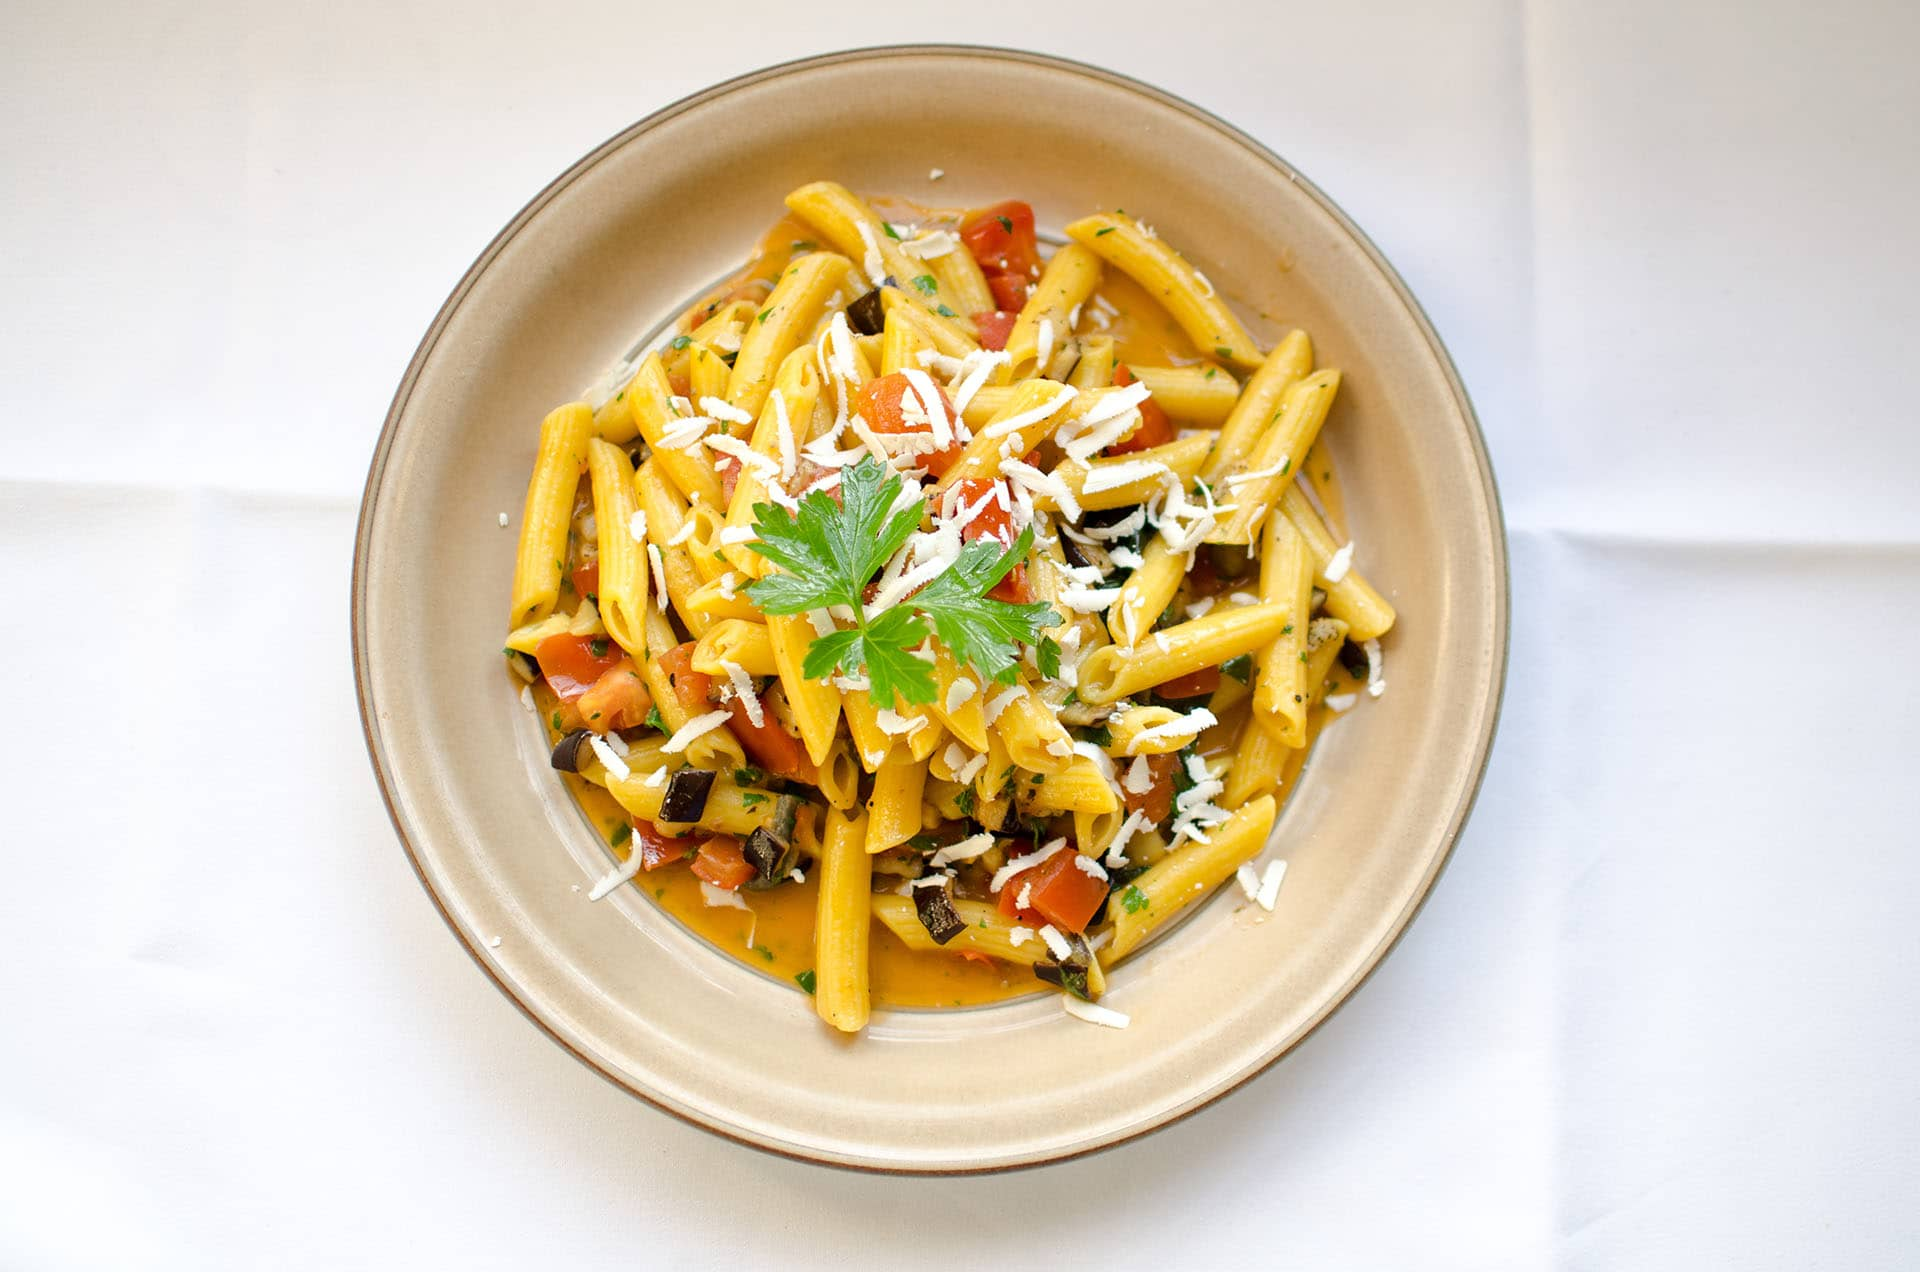
\includegraphics[width=\textwidth]{img/penne.jpg}
  \caption{Ukázka popisovaného obrázku}
  \label{fig:penne}
\end{figure} 

\begin{lstlisting}[caption=Ukázka vyplnění \texttt{alt} atributu elementu \texttt{<img>},label=fig:img]
	<img src="./img/pennenorma.jpg" alt="Penne alla Norma at La Casa Degli Amici, author: Martin Knapovsky" />
\end{lstlisting}

Minifikaci lze provádět ručně - existuje mnoho online řešení (např. \url{https://cssminifier.com}), automatizovaně při každé úpravě souboru (např. pomocí systému Gulp\footnote{\url{http://gulpjs.com}}), nebo také plně automaticky pomocí \textbf{PageSpeed} modulu pro webový server Apache a Nginx\footnote{\url{https://developers.google.com/speed/pagespeed/module/}}. Výhoda PageSpeed modulu spočívá v jeho síle - dokáže automaticky minifikovat soubory typu CSS a JS, komprimovat přenášená data pomocí \textbf{gzip komprese}, dokáže redukovat velikost obrázků a také podporuje \textbf{cachování} - stránky vygenerované pomocí PHP interpretace uloží ve statické podobě a ty jsou následně při HTTP dotazu odeslány uživateli. Jedná se tak o zkrácení času potřebného pro odpověď serveru na uživatelský požadavek na načtení webových stránek.\\

\textbf{Responzivní design}
\label{section:responsive}

Jak již bylo uvedeno v kapitole \ref{section:mobileshift}, mobilní zařízení v počtu provedených vyhledávání předehnala klasické desktopy a vyhledávač Google začal posuzovat responzivitu webových stránek jako jeden ze signálů pro ohodnocení. Responzivní web se \textbf{přizpůsobuje mobilním zařízením} s malým displayem a umožňuje s ním na takovém zařízení \textbf{komfortně pracovat}. V dobách, kdy se začínaly objevovat první mobilní zařízení s internetovým prohlížečem, začaly se hledat cesty, jak do těchto zařízení doručit obsah stávajícíh webových stránek. Z počátku se vytvářely samostatné mobilní weby, na které byl uživatel přesměrován, pokud dotazovaný server zjistil, že je uživatel na mobilním zařízení. Takový přístup se ukázal jako komplikovaný, jelikož musely být spravovány 2 separátní weby - data, funkcionalita, obsah, a tak dále. S tímto přístupem se dnes již setkáváme málokdy - už jenom z toho důvodu, že separátní weby si \textbf{přerozdělují ohodnocení} vyhledávače, které by mohl získat jeden web samotný (viz PageRank algoritmus - \ref{section:pagerank}). Podíváme-li se na statistiky používaných rozlišení zařízení \ref{table:widthsdesktop}, zjistíme, že nejpoužívanějším rozlišením je 640x360 pixelů, což odpovídá jednoznačně mobilním telefonům. Růst tohoto rozlišení a potvrzení statistik v tabulce je možné vidět na obrázku \ref{fig:gsresolution}. V souvislosti s faktem, že mobilní zařízení překonala ve vyhledávání desktopy, vidíme, že responzivní design webových stránek je dnes velmi důležitý. 

\begin{table}[]
\centering
\label{table:widthsdesktop}
\begin{tabular}{lll}
1  & 640x360   & 18.02 \% \\
2  & 1366x768  & 15.66 \% \\
3  & 1024x768  & 8.84 \%  \\
4  & 1920x1080 & 7.18 \%  \\
5  & 667x375   & 4.97 \%  \\
6  & 568x320   & 4.37 \%  \\
7  & 1280x800  & 3.76 \%  \\
8  & 1600x900  & 3.10 \%  \\
9  & 1440x900  & 3.06 \%  \\
10 & 534x320   & 2.90 \% 
\end{tabular}
\caption{Tabulka nejvíce používáných rozměrů zobrazovacích zařízení, zdroj: W3Counter, 10/2016}
\end{table}

\begin{figure}
  \centering
    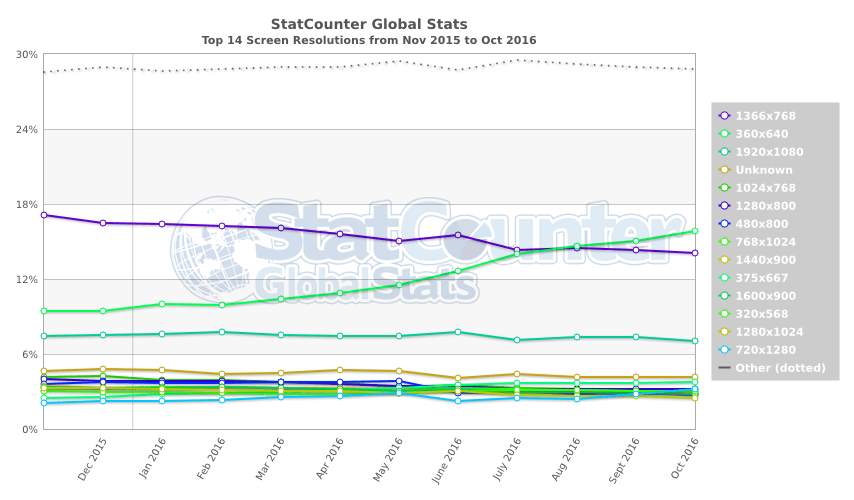
\includegraphics[width=\textwidth]{img/gsresolutions.png}
  \caption{Rozlišení používaná od 11/2015 do 10/2016}
  \label{fig:gsresolution}
\end{figure} 

Responzivní design využívá tzv. \texttt{media-queries}, což je vlastnost CSS definovat rozměry obrazovek, na kterých se má web zobrazovat například v jednosloupcovém rozložení a rozměry, ve kterých se bude zobrazovat ve vícesloupcovém rozložení. Docílíme tak toho, že se responzivní web na zařízení s malým displayem \uv{přeskládá}, aby byl pro uživatele lépe použitelný. Velikostem obrazovky, na kterých se web \uv{přeskládává} (mění svůj \textit{layout}) se říká \textbf{breakpoints}. Změnou rozložení však responzivita nekončí. Obrazovky mobilních zařízení bývají často dotykové, obrazovky desktopů nikoliv. Pomocí media-queries lze také změnit chování webu (JavaScriptová funkcionalita) a umožnit uživateli ovládání pomocí dotyků (např. responzivní obrázkový \uv{slider}). Pokud bychom na mobilním telefonu měli čekat na načtení obrázku s rozlišením 3440x1440px, trvalo by načítání značně dlouhou dobu a velikost načteného obrázku bychom ani nevyužili (obrázek se stejně zobrazí na obrazovce s malým rozlišením). Ideální způsob optimalizace obrázků je vytváření \textbf{několika verzí pro různá zařízení}. Server, na kterém jsou stránky umístěny, se dozví (z HTTP dotazu, nebo pomocí JavaScriptu), že dotaz na načtení stránek je směrován ze zařízení s malým displayem a dodá tak obrázky v menších velikostech. Pro velký FULLHD (1920x1080px) display pak server dodá obrázky větších rozměrů. Pro jednotlivé velikosti obrázků jsou často voleny maximální šířky zobrazovacího zařízení. \\

\textbf{Příklad}:\\
Původní neupravený obrázek má rozlišení s šířkou 3000px. Tento soubor má velikost 4MB. Media-query breakpoint máme stanovený na 1280px a na 1920px. To znamená, že při šířce zobrazovacího zařízení, která spadá mezi tyto breakpointy, se bude naše stránka zobrazovat ve stejném rozložení (layoutu) a se stejným obsahem - se stejným obrázkem. Zařízení s velmi častou zobrazovací šířkou 1366px spadá do těchto mezí a naše stránka tedy bude vypadat stejně jako na obrazovce se zobrazovaní šířkou 1920px. Přípravíme si obrázky pro zobrazení na obrazovce s šířkou menší než 1280px, menší než 1920px a původní obrázek v komprimované podobě (jpeg). Velikosti souborů a jejich šířky jsou: 1280px (75kB), 1920px (200kB) a původní se šířkou 3000px (700kB). Na našem zařízení se šířkou 1366px použijeme obrázek se šířkou odvídající největší možné velikosti obrazovky, kde je dané rozložení platné - 1920px. Obrázek se zmenší dle velikosti zařízení a my jsme tak ušetřily 500kB oproti načítání obrázku v původní velikosti. Na mobilním zařízení s šířkou  obrazovky 640px bychom ušetřily ještě více (615kB). Obrázek není zvětšený a je tedy zobrazený v dobré kvalitě. 

Tématika responzivního designu je obsáhlá a pro tuto práci není hlavním tématem - čtenáři postačí vědět, že něco takového je možné a že je to vhodné pro SEO a také UX. Příklad řešení optimalizace velikosti obrázků si ukážeme v praktické části diplomové práce. \\ 

\textbf{URL adresa}

Častou chybou je vytváření duplicítních URL adres, které vyhledávací robot nechápe jako 1 stránku, ale jako více různých stránek s duplicitním obsahem. V následku toho se díky duplicitnímu obsahu sníží ohodnocení jednotlivých stránek. Může se jednat například o tyto případy:

\begin{itemize}
	\item \texttt{http://www.example.com}
	\item \texttt{http://www.example.com/index.php}
	\item \texttt{http://www.example.com/home}
	\item \texttt{http://example.com}
	\item \texttt{http://example.com/index.php}
	\item \texttt{http://example.com/home}
	\item \texttt{https://example.com/home}
	\item \texttt{https://www.example.com}
	\item a další kombinace
\end{itemize}   

Řešení se nabízí v použití \texttt{mod\_rewrite} modulu pro webový server Apache\footnote{dostupný z \url{https://httpd.apache.org}}. Pomocí tohoto modulu lze vytvářet podmínky pro přepisování adres tak, aby se při zadání např. \texttt{example.com} či \texttt{www.example.com} URL adresa vždy přepsala na \texttt{https://\-www.example.com/\-home}, kterou jsme určily jako hlavní URL pro přístup na domovskou stránku.

\begin{comment}
\begin{lstlisting}[caption=Ukázka jednoduchého \texttt{mod\_rewrite} pravidla,label=code:modrewrite]
<IfModule mod_rewrite.c>
	RewriteEngine On
	RewriteBase /
	RewriteRule ^index\.php$ - [L]
	RewriteCond %{REQUEST_FILENAME} !-f
	RewriteCond %{REQUEST_FILENAME} !-d
	RewriteRule . /index.php [L]
</IfModule>
\end{lstlisting}
\end{comment}

Další požadavek na URL adresu je její \textbf{srozumitelnost}. To, jak URL adresa vypadá, není přímo hodnocím signálem vyhledávače, avšak URL adresa je uživateli zobrazena ve výsledcích vyhledávání a je tedy vhodné, aby byla dobře čitelná. To, jakým způsobem se adresa vytváří, je možné opět ovlivnit v \texttt{.htaccess} souboru pomocí modulu mod\_rewrite.\\

Příklady:
\begin{enumerate}
	\item \texttt{https://www.knapovsky.com/?p=123}
	\item \texttt{https://www.knapovsky.com/aplikace-seo-pro-marketing/}\\
\end{enumerate}

Z příkladů je jasné, že vhodnější je varinta 2, která hned na první pohled odhaluje co se na odkazované stránce nachází.

Velice důležitým prvem SEO je \textbf{udržování statických URL adres}. Pokud vyhledávač jednou naindexuje webovou stránku s určitou URL (například první z příkladů výše) a my pak změníme strukturu URL (příklad č. 2), ztratíme původní ohodnocení stránky. Pokud navíc nezakomponujeme nějaký typ přesměrování ze starého odkazu na nový, ztratíme zpětné odkazy, které jsou stále jedním z nejdůležitějších faktorů pro ohodnocení stránek (kapitola \ref{section:offpageanalysis}). 

\newpage
\textbf{Analýza klíčových slov}

Analýza klíčových slov pomocí SEO nástrojů (\ref{section:seotools}) dokáže odhalit to, \textbf{co lidé nejčastěji vyhledávají a co je zajímá}. Získáme tím přehled o uživatelských strategiích a optimalizací tak připravujeme webové stránky k tomu, aby šli stránky uživatelům vyhledávačů naproti a aby stránky uspokojily jejich poptávku. Při analýze klíčových slov je nutné brát ohled na konkurenci, která již používá klíčová slova, na která se chceme v optimalizaci soustředit. Zvolení špatných klíčových slov může skončit velmi dobrým ohodnocením při klíčových slovech, které nikdo nehledá. Několik minut přemýšlení nad správnými slovy může ušetřit několik měsíců zbytečné práce na optimalizaci webu. 

\label{section:keywordstuffing} 
Jak již bylo uvedeno v kapitole \ref{section:onpageanalysis}, vyhledávače primárně analyzují klíčová slova v \texttt{<title>} HTML tagu, dále v nadpisech - \texttt{<H1>}, \texttt{<H2>}, \texttt{<H3>} atd., v textu odkazů a také v samotném obsahovém textu stránky. Větší váha se přikládá také slovům, které jsou obsaženy v \texttt{<strong>}, \texttt{<b>}, \texttt{<i>}, \texttt{<u>} a \texttt{<meta>}  HTML tagu. U jednotlivých HTML tagů záleží na jejich hustotě (jak často se na stránce vyskytují) a také jak daleko od HTML tagu \texttt{<body>} jsou umístěny. Čím blíže, tím lépe. Obsah \texttt{<meta name='description'>} tagu je použit pro popis vyhledané stránky (obrázek \ref{fig:toolongtitle}) a zdrojový kód \ref{code:title}. Při přesažení určité hustoty klíčového slova je stránka penalizována. Jedná se black-hat SEO techniku, která je nazývaná \textbf{keyword stuffing}. Tato technika byla používaná v dřívějších dobách, avšak dnes již pro optimalizaci není díky aktualizacím vyhledávacích algoritmů použitelná. 

\textbf{Titulek} se zobrazuje ve výsledcích vyhledávání a měl by tedy být \textbf{výstižný}, \textbf{stručný} a \textbf{jedinečný}. Zároveň by neměl přesáhnout délku 55 znaků - více znaků stejně vyhledávač neanalyzuje\footnote{\url{https://moz.com/learn/seo/title-tag}}. Ukázka dlouhého titulku ze zdrojového kódu \ref{code:title} je na obrázku \ref{fig:toolongtitle}. \\

\begin{lstlisting}[caption=Ukázka dlouhého titulku v \texttt{<title>} elementu,label=code:title]
<!DOCTYPE html>
<html>
  <head>
    <title>Ukazka velmi dlouheho titulku, ktery presahuje 55 znaku a je nalezite oriznut</title>
    <meta name="description" content="This is your page description. The font and size of the description has not changed in the latest redesign. Descriptions get cut off after roughly 160 characters and the rest of the description is not visible."/>
  </head>
</html>
\end{lstlisting}

\begin{figure}
  \centering
    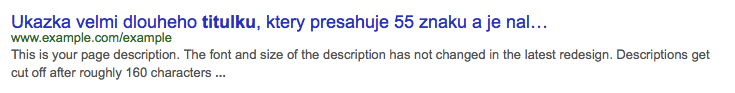
\includegraphics[width=\textwidth]{img/toolongtitle.png}
  \caption{Ukázka ořezu dlouhého titulku}
  \label{fig:toolongtitle}
\end{figure} 

Na obrázku \ref{fig:toolongtitle} je také možné si všimnout, že je tučným písmem zvýrazněno slovo \textbf{titulku}. To je z toho důvodu, že slovo \uv{titulku} bylo původním vyhledávacím řetězcem a vyhledávač označuje slova, která se vyskytovala ve vyhledávacím řetězci.

Váha klíčového slova je určena jeho důležitostí na stránce - je-li například v titulku stránky pět slov, rozděluje se důležitost mezi těchto pět slov. Vzhledem k tomu, že vyhledávače implementují sémantické vyhledávání (kapitola \ref{section:keywordanalysis}), nezáleží dnes už pouze na tom jaká slova jsou použita, ale také na celkovém sémantickém významu webové stránky. Vyhledávač může sémantickou analýzou do určité míry pochopit obsah stránky a může tedy mezí výsledky vyhledávání nabídnout i stránky, které přesně vyhledávaná klíčová slova neobsahují, avšak týkají se stejného tématu, které uživatel vyhledává.

Nemá smysl jedinou stránku optimalizovat pro 15 klíčových slov, protože váha každého samostatného klíčového slova bude tak malá, že bude pro vyhledávacího robota zanedbatelná. V případě optimalizace pro více klíčových slov je vhodnější pro každé důležité klíčové slovo vytvořit vlastní stránku s unikátním obsahem souvisejícím s tématikou vybraného klíčového slova \cite{Komarek2009}.

Pro analýzu klíčových slov lze použít několik nástrojů. Většina z uvedených nástrojů ukazuje statistiky o tom, jak je dané klíčové slovo používané, navrhují alternativní možnosti, analyzují ohodnocení nejlepších vysledků a množství vyhledávání pro analyzované klíčové slovo. V následujícím přehledu jsou uvedeny některé z nástrojů určených k analýze klíčových slov. Další SEO nástroje jsou uvedeny v kapitole \ref{section:seotools}.

Nástroje:
\begin{itemize}
	\item Moz keyword explorer\footnote{\url{https://moz.com/explorer}}
	\item Google AdWords Keyword Planner\footnote{\url{http://adwords.google.com/keywordplanner}}
	\item Google Trends\footnote{\url{http://www.google.com/insights/search/}}
	\item Microsoft Bing Ads Intelligence\footnote{\url{http://advertising.microsoft.com/small-business/adcenter-downloads/microsoft-advertising-intelligence}}
	\item Wordtracker's Free Basic Keyword Demand\footnote{\url{https://freekeywords.wordtracker.com/}}
\end{itemize}

\begin{comment}
\textbf{Tvorba obsahu}
\label{section:qualitycontent}

\todo{Napsat o tvorbe kvalitniho obsahu}
K úspěchu ve vyhledávačích je nutné vytvoření kvalitního a unikátního obsahu tak aby uspokojil poptávku a aby ho lidé sdílely. 

problem prihlaseni


Make a reasonable effort to ensure that advertisement links on your pages do not affect search engine rankings. For example, use robots.txt or rel="nofollow" to prevent advertisement links from being followed by a crawler.

Ensure that  your site appears correctly in different browsers.

If possible, secure your site's connections with HTTPS. Encrypting interactions between the user and your website is a good practice for communication on the web. 
\end{comment}

\newpage
\subsubsection{Off-page SEO}

\uv{Jedním z nejsilnějších parametrů pro řazení výsledků ve vyhledávači je počet a kvalita zpětných odkazů (to jsou odkazy z jiných stránek na váš web). Je to vcelku logické. Můžete mít skvěle optimalizovaný web, ale o jeho kvalitě rozhodují návštěvníci. Pokud na web vede řada odkazů z kvalitních webů, znamená to, že je kvalitní.}\cite{Grimmich}

Jak bylo uvedeno v kapitole o algoritmu PageRank (\ref{section:pagerank}), čím více kvalitních odkazů tím lépe. Budování odkazů lze dělat různými způsoby. Obecně však platí to, že nejlepší je tvorba kvalitního obsahu, který lidé sdílí, píší o něm, komentují ho a popularita stránek tak vzrůstá. \\

\textbf{Tvorba mikrostránek}

Mikrostránky jsou úzce zaměřeny na propagaci jednoho produktu, či tématu a mají za cíl získávat zpětné odkazy z tématicky zaměřených webů a odkazovat na hlavní webovou prezentaci, kterou mikrostránky posilují. Mikrostránky jsou používány k zveřejňování \uv{efektivních článků} - mohou zvýraznit nový produkt nebo technologii, nebo se například může jednat o mikrostránku věnovanou druhům koření v italské kuchyni, ve které jsou umístěny odkazy na posilovanou italskou restauraci. Opět však nejde o to, abychom do stránky vkládaly vysoké množství odkazů a klíčových slov - jde primárně o kvalitní obsah. Jak jsme si ukázali v kapitole \ref{section:howpeoplesearch}, lidé používají různé vyhledávací strategie, díky mikrostránkám mohou získat potřebné informace a pokud bude obsah dobře zpracován, je pravděpodobné, že si zakoupí produkt na našem hlavním webu.\\

\textbf{Zveřejňování článků} 

Blogové články sloužit k zisku hodnotných zpětných odkazů. Články by měly být zveřejňovány na tématicky podobných zpravodajských/blogových stránkách. Získáme tak vyšší ohodnocení a také jsou naše stránky mnohem blíže lidem, kteří se zajímají o danou tématiku.\\

\textbf{Sociální sítě}

Dnes velmi častý způsob propagace. Na sociálních sítích se obsah (s odkazem na naši stránku) může šířit velmi rychle bez nutnosti našeho zásahu. Pokud lidem poskytneme kvalitní obsah, který je zaujme natolik, že ho sdílí, rozšíří se tak naše publikum o ty, kteří jsou na sociální síti se sdílejícím uživatelem v přátelském vztahu (nebo ho minimálně nějak sledují). Pravidelným dodáváním obsahu do sociálních sítí se udržujeme v povědomí a zvyšujeme tak pravděpodobnost, že si od nás zákazník něco koupí. Sociální sítě jsou dnes také prostředkem s vysokým dosahem. Podle článku zpravodajského deníku Telegraph\footnote{\url{http://www.telegraph.co.uk/technology/2016/02/04/facebook-says-there-are-actually-357-degrees-of-separation/}} má sociální síť Facebook už průměrně pouze 3,57 stupňů odloučení, což znamená, že lze od jakéhokoliv uživatele dojít přes jeho přítele, který má další přátele ke komukoliv jinému v této síti. Globálně nyní v průměru potřebujeme projít pouze přes 3,57 uživatelů. Využití sociálních sítí bude ukázáno v praktické části.\\

\newpage
\textbf{Výměna odkazů} 

Výměna odkazů je dohoda mezi dvěma weby o vzájemném umístění zpětného odkazu. Jedná se o velice populární metodu získávání zpětných odkazů. Odkazy se umisťují do patičky, nebo se vytváří určitá partnerská sekce.
Odkazy lze také nakupovat - vyhledávače však takovou činnost považují za nepovolenou techniku a při jejím odhalení stránky penalizují.\\ 

\textbf{Registrace stránek do katalogů}

Umístěním stránek do různých katalogů lze také zvýšit ohodnocení stránek. Nevýhodou katalogů je, že obsahují spoustu odkazů a ohodnocení, které z nich získáme tak tedy není tak vysoké (\ref{section:pagerank}). Příkladem českého katalogu jsou \url{firmy.cz}, které spadají pod český vyhledávač \url{www.seznam.cz}, mezi globálně používané katalogy spadá např. \url{www.yelp.com} a \url{www.yahoo.com}.

Dalšími vhodným způsobem tvorby zpětných odkazů je \textbf{přispívaní do diskuzních fór a komentování} různých tématických příspěvků na zpravodajských serverech a blogu. Je však potřeba mít na paměti, že se často jedná o zpětné odkazy, které obsahují \texttt{nofollow} atribut udávající vyhledávači informaci o tom, že takový odkaz nemá při ohodnocování cílových stránek započítávat (kapitola \ref{section:nofollow}).

\subsubsection{Black-hat SEO}
\label{section:blackhatseo}

Black-hat SEO je označení pro množinu SEO technik, které neetickým způsobem zneužívají mezery algoritmů vyhledávače tak, aby získaly co nejlepší ohodnocení. Souboj vyhledávačů a black-hat SEO je veden od dob kdy obě tyto oblasti vznikly. Jak jsme mohli vidět v popisu historie vyhledávačů (\ref{section:searchenginehistory}) a v popisu vyhledávacích algoritmů (\ref{section:anatomy}), je to právě black-hat SEO, které podněcuje vývoj některých vyhledávacích algoritmů (Google Panda, Google Penguin, ...). 

Google Webmaster Guidelines\footnote{\url{https://support.google.com/webmasters/answer/35769?hl=en}} představují doporučení, která by se při tvorbě webů a jejich SEO měla používat. Stránky uvádí následující body:

\begin{itemize}
	\item Vytvářejte stránky především pro uživatele, nikoli pro vyhledávače.
	\item Neoklamávejte uživatele.
	\item Nepoužívejte triky, které mají za cíl zvýšit hodnocení ve vyhledávačeích. Obvykle je dobré zamyslet se, zda by vám nevadilo, kdyby se o vašem jednání dozvěděli správci konkurenčního webu nebo zaměstnanci společnosti Google. Další vhodné otázky jsou \uv{Pomáhám tímto svým uživatelům? Dělal(a) bych to, kdyby vyhledávače neexistovaly?}
	\item Zamyslete se, co dělá vaše webové stránky jedinečnými, hodnotnými a poutavými. Snažte se, aby vaše stránky oproti ostatním stránkám v oboru vynikaly. 
\end{itemize}

Stránky, které tyto doporuční následují mají jistotu, že nebudou nijak penalizovány. Při odhalení jakékoliv použité black-hat techniky jsou pak stránky penalizovány nízkým ohodnocením.

V následující několika odstavcích si ukážeme jaké techniky black-hat SEO používá. Je nutno zmínit, že techniky, které black-hat SEO používá, je velké množství a jsou známy ty, na které se vyhledávače zaměřují. Mnoho z nich však stále ovlivňuje ohodnocování webů. Vyhledávače o nich neví, nebo nemají způsob, jakým by je odhalily.\\

\textbf{Automaticky generovaný obsah}
\label{bh:generatedcontent}

Automaticky generovaný obsah je obsah, který byl vygenerován programem. Obsah často nemá žádný sémantický význam a zaměřuje se na to, aby obsahoval vyhledáváná klíčová slova.

Příklady:
\begin{itemize}
	\item Automaticky přeložený text bez korektury člověkem
	\item Text generovaný pomocí automatických procesů, jako jsou Markovovy řetězce
	\item Text generovaný pomocí technik synonymizace a obfuskace
	\item Text vygenerovaný extrakcí z Atom nebo RSS zdrojů
	\item Text generovaný z výsledků vyhledávání
	\item Text vzniklý kombinováním obsahu z různých webových stránek bez přidání dostatečné hodnoty\\
\end{itemize}

\textbf{Manipulativní odkazování}
\label{bh:linking}

Jednou z nejvíce populárních technik black-hat SEO je zisk zpětných odkazů pomocí spamu. Algoritmy pro odhalování takových technik jsou stále pokročilejší (kapitola \ref{section:penguin}), avšak stále nejsou dokonalé a spamu je mezi výsledky velké množství. 

Může se jednat o tyto techniky:
\begin{itemize}
	\item Koupě nebo prodej odkazů za účelem zvýšení ohodnocení v algoritmu PageRank (\ref{section:pagerank}). Patří sem platba za odkazy, výměna zboží nebo služeb za odkazy i zaslání produktu zdarma výměnou za to, že o vás příjemce napíše a bude na vás odkazovat. 
	\item Rozsáhlá výměna odkazů nebo vytváření partnerských stránek výlučně za účelem vzá\-jem\-ného odkazování.
	\item Používání automatizovaných programů nebo služeb k vytváření odkazů na stránky za účelem zisku lepšího ohodnocení (jedná o tzv. linkové farmy, které jsou vytvořeny čistě pro manipulaci ohodnocení vyhledávače)
	\item Odkazy vkládané do widgetů, které jsou distribuovány na různé stránky (např. widget zobrazující počet návštěvníků a odkaz na pojištění automobilů)
	\item Reklamy předávající PageRank ohodnocení (reklamy by měly využívat \texttt{rel="nofollow"} atributu)
	\item Komentáře na blogu nebo diskuzích, které používají optimalizované odkazy (u komentářů by se opět měl používat \texttt{rel="nofollow"} atribut) \\
\end{itemize}

\textbf{Cloaking}
\label{bh:cloaking}

Vyhledávací robot není člověk a prochází primárně zdrojový kód stránek, ve kterém toho může nalézt více, než by se dalo očekávat. V některých případech je tato technika povolená (např. pro alternativní text k flash animaci, kterou by vyhledávač neměl jak jinak analyzovat), avšak často je této techniky využívano ke skryvání bloků textu, do kterých se dosazují klíčová slova, která vidí pouze vyhledávač a uživatel nikoliv.
Může se jednat o bílý text na bílém pozadí, o použití malé velikosti písma, nebo o použití \texttt{visibility: none} a dalších podobných CSS stylů.\\

\textbf{Podvodná přesměrování}
\label{bh:redirects}

Přesměrování lze využít pro dobré účely - stránky se přesunují z jedné domény na druhou, URL se mění a my potřebujeme zajistit, aby se lidé se starým odkazem stále dostali k našemu obsahu - použijeme tedy přesměrování. Přesměrování lze však využít také tím způsobem, že je podmíněno typem parametru \texttt{user-agent}, který udává z jakého prohlížeče uživatel prochází stránky a lze pomocí něho i odhalit, že ten, kdo požaduje načtení stránek je vyhledávač, který pomocí svého vyhledávacího robota analyzuje stránky. Jsme tak schopni poskytnout vyhledávači jiný obsah než uživateli a toho je při podvodném přesměrování využíváno. Na stránkách určených pro vyhledávač budou obsažena klíčová slova, pro která chceme náš web ohodnotit. Pomocí této techniky se tak mezi výsledky vyhledávání mohou \uv{protlačit} stránky s původním hledáním nesouvisející - hazardní gambling, prodej snubních prstenů či viagry. 

\subsection{Vyhodnocení SEO}
\label{section:seoreview}

Nejlepším způsobem, jak měřit efektivnost SEO optimalizace, je porovnání návštěvnosti stránek a pozice v SERP na hlavní klíčová slova před SEO optimalizací a po ní. Ovšem hrubý počet návštěvníků, kteří přijdou na stránky, rozhodně nestačí \cite{Komarek2009}. Musíme brát ohled na to, že SEO bývá často prováděno v širším marketingovém kontextu. Kampaně jako různé newslettery, akce a letáky zvyšují návštěvnost a pro vyhodnocení jednotlivých kampaní je vhodné pro každou kampaň vytvořit unikátní URL adresu, přes kterou uživatelé na naše stránky přicházejí. Tím získáme informaci o úspěšnosti jednotlivých kampaní a můžeme lépe vyhodnotit úspěch samotné SEO optimalizace. 

Je přirozené, že se návštěvnost a prodeje mění v závislosti na sezóně. Pokud budeme posuzovat návštěvnost obchodu s dárkovými předměty, bude návštěvnost a prodej jistě vyšší v prosinci než v lednu. Ideální je meziroční sledování díky kterým můžeme odfiltrovat vliv sezónních trendů.

Dalším důležitým faktorem jsou společenské změny - může se jednat o ekonomické recese, změnu vlády, změnu zákona, růst nezaměstnanosti, růst inflace, atd.

Pro vyhodnocení úspěšnosti SEO používáme nástroje, díky kterým lze sledovat mnoho růz\-ných faktorů ovlivňujících kvalitu aplikace SEO. V následujících odstavcích si několik z nich před\-sta\-víme.

\newpage
\subsection{SEO nástroje}
\label{section:seotools}

\subsubsection{Google Analytics}
\label{section:analytics}

Data přímo od zdroje. Google Analytics sbírá informace o návštěvnosti, které nekončí pouhým počtem příchozích, ale také ví z jakého prohlíče uživatelé přistupovali, z jakého zařízení a operačního systému, z jakého města a mnoho dalších informací, dle kterých lze vyhodnotit na které sociální skupiny vaše stránky nejvíce působí, jaký má vaše marketingová strategie dosah a jak se SEO vyplácí. Google Analytics budeme používat pro vyhodnocení v praktické části.

\subsubsection{Google PageSpeed Insights}
\label{section:pagespeedinsights}

Google PageSpeed Insights analyzuje stránky z pohledu jejich optimalizace pro načítání a posuzuje různé faktory:

\begin{itemize}
	\item Velikost souborů
	\item Odezvu serveru
	\item Kvalitu optimalizace obrázků
	\item Rychlost spouštění JavaScriptu
	\item Responzivitu webu
	\item Kvalitu optimalizace načítání externích souborů
\end{itemize}

Data z hodnocení různých faktorů jsou agregována do celkového hodnocení od 0 do 100. Tento nástroj také v případě špatné optimalizace CSS a JS souborů umožňuje stažení jejich optimalizovaných verzí. Tento nástroj budeme používat pro vyhodnocení SEO v praktické části.

\subsubsection{Moz Local Listing Score}
\label{section:mozlocallisting}

Tento nástroj vyhodnocuje informace z více než 15 různých různých sítí jako Foursquare či Facebook a ukazuje nám slabiny, na které bychom se měli při optimalizaci zaměřit. Mnoho návštěvnosti dnes na webové stránky proudí ze sociálních sítí a bez jejich využití se tak ochuzujeme o možný zisk.

\subsubsection{Google Webmaster Tools a Bing Webmaster Tools}
\label{section:webmaster}

Webmaster tools od společnosti Google i Bing slouží k analýze indexace webových stránek. Pomocí těchto nástrojů odhalíme, že se některé z našich stránek neanalyzovaly, nebo že se stránky nelze dobře analyzovat díky obsahu, který je dostupný až po přihlášení, nebo díky příliš komplexnímu JavaScriptu. Pomocí těchto nástrojů lze také vyhledávači odeslat XML sitemapu, pomocí které může vyhledávač lépe indexovat stránky - můžeme tak i vyhledávači předat informace o stránkách, které by normálním crawlingem nenašel. Tento nástroj budeme také používat v praktické části.

\subsubsection{ahrefs}
\label{section:ahrefs}

Tento nástroj je takovým švýcarským nožem mezi SEO nástroji. Je rozdělen mezi několik sekcí:

\begin{itemize}
	\item \textbf{Site Explorer} - Analyzátor zpětných odkazů pro daný web či jednotlivé stránky a analýza síly jednotlivých odkazů. Nástroj sbírá data dlouhodobě a vytváří přehledy v podobě grafů a tabulek.
	\item \textbf{Position Explorer} - Analýza konkurence - Nástroj dokáže analyzovat pozice v SERP pro jednotlivá klíčová slova, dokáže odhalit zda konkurence používá placenou reklamu, kolik za ni platí a také ze kterých stránek získává konkurence nejvíce návštěvnosti. 
	\item \textbf{Content Explorer} - Dokáže ohodnotit kvalitu obsahu a porovnat ji s obsahem konkurence.
	\item \textbf{Position Tracker} - Tento nástroj slouží pro analýzu ohodnocení a pozice ve vyhledávači pro konkrétní klíčová slova, která v nástroji necháme sledovat.
	\item \textbf{Crawl Report} - Dokáže odhalit problémy s analýzou obsahu, které mohou nastat ve chvíli, kdy používáme množství JavaScriptu, nebo nepoužíváme validní HTML syntaxi.
	\item \textbf{Ahrefs alerts} - Skvělý nástroj, který dokáže odhalit nově zveřejněný odkaz na naše stránky a upozornit nás o tom emailem. 
\end{itemize} 

\begin{figure}
  \centering
    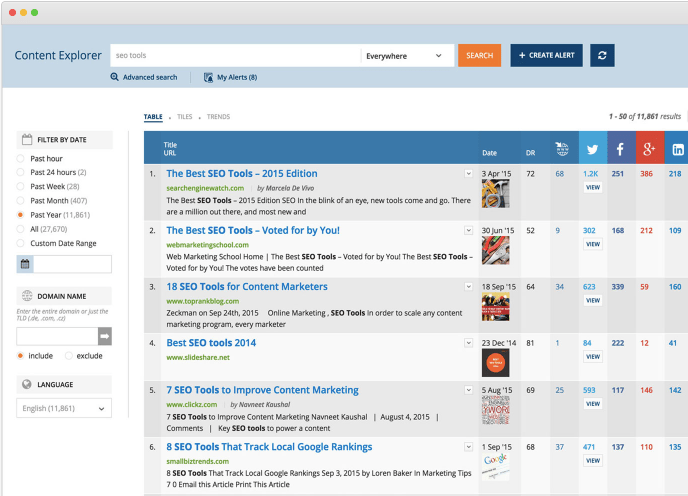
\includegraphics[width=\textwidth]{img/ahrefscontent.png}
  \caption{ahrefs Content Explorer, zdroj: ahrefs.com}
  \label{fig:ahrefscontent}
\end{figure}

Jedná se placený nástroj, který se vyplatí pro pokročilou SEO analýzu.

%\subsection{Budoucnost SEO}
%V kapitole \ref{section:anatomy} jsme si uvedli, jak rychle se mění algoritmy vyhledávačů a jak se stále snaží dosahovat vyšší relevantnosti mezi výhledáváním a výsledky. Vyhledávače se snaží algoritmy uzpůsobit tak, aby jejich ohodnocení bylo co nejpřesnější a SEO tak musí měnit přístupy, které používá.
\subsection{Shrnutí}
V kapitole \ref{section:SEO} byla představena optimalizace pro vyhledávače, její výhody, strategie, techniky a nástroje. SEO je po emailu nejdůležitějším online marketingovým nástrojem a jeho použití se stává nutností. V textu byly uvedeny hlavní techniky, které se dnes pro optimalizaci používají a byly představeny také black-hat SEO techniky, které hledají mezery ve vyhledávacích algoritmech a využívají jich. Znalosti získané v této kapitole budou společně s uvedenými nástroji využity v praktické části.

\section{Shrnutí popisné a úvahové části}
V rámci kapitoly \ref{section:theory} byl prezentován pohled na 3 subjekty, které přicházejí s vyhledáváním do styku - samotný vyhledávač, uživatel a SEO, které reprezentuje webové stránky a jejich snahu umístit se ve výsledcích vyhledávače na předních pozicích. V části o vyhledávačích jsme si ukázali vazbu mezi vyhledávačem a uživatelem a vazbu mezi vyhledávačem a SEO. Vyhledávače jsou přizpůsobovány tak, aby dosáhly největší možné relevance výsledků vůči uživatelskému dotazu a také aby ze svých výsledků odstranily spam, který často vzniká jako důsledek použití black-hat SEO technik, které nemorálním způsobem ovlivňují pořadí výsledků vyhledávače. Rozvoj těchto technik podněcuje rozvoj vyhledávačů a jejich algoritmů. Z textu už také víme, jakým způsobem vyhledávače pracují - procházejí síť WWW, analyzují jednotlivé webové stránky a vytváři si abstraktní reprezentaci sítě - index, pomocí kterého následně hledají odpovědi na uživatelské dotazy. Podborně jsme si představili algoritmus PageRank, jehož výsledek ohodnocení je jedním z hlavních signálů, pomocí kterého vyhledávač ohodnocuje a řadí nalezené výsledky. V Kapitole \ref{section:howpeoplesearch} jsme si ukázali, že dostat svůj web mezi přední výsledky vyhledávání je pouze prvním krokem k úspěchu. Uživatelé mohou provádět nekolikanásobná vyhledávání a teprve poté provádějí akci (zisk požadované informace, nákup, registrace, ...) - k úspěchu je potřeba vybudovat celý ekosystém online prezentace nebo rozšířit marketingovou strategii o další prvky, které dodají člověku důvěru k provedení akce. V kapitole \ref{section:SEO} jsme si pak ukázali možnosti optimalizace webových stránek tak, aby se jejich obsah přiblížil co možná nejvíce lidem schopných konverze. Techniky se zaměřují na on-page optimalizaci, která analyzuje a implementuje optimalizaci obsahového textu, obrázků, URL adres či velikosti dat a off-page optimalizaci, která využívá znalosti algoritmu PageRank a dalších signálů, které vyhledávač používá při řazení výsledků vyhledávání. Kapitola \ref{section:theory} je důležitá pro pochopení návrhu a implementace marketingové strategie v praktické části.     

\chapter{Praktická část}
\label{section:practical}

Praktická část se zabývá návrhem a implementací marketingové strategie obsahující tvorbu webu, SEO a propagaci na sociálních sítí pro italskou restauraci \textbf{La Casa Degli Amici}. Tato restaurace sídlí v jihovýchodním Londýně na adrese \textbf{196 Norwood Road, SE279AU} a jejím vlastníkem je \textbf{Thomas Fiala} (lacasadegliamici@hotmail.com, +44 (0) 7809 463263). Restaurace poptávala vytvoření webu a propagaci na sociálních sítích k rozšíření povědomí o restauraci. Konečný cílem je samozřejmě navýšení zisku restaurace. Ukážeme si návrh webu, jeho implementaci, implementaci SEO a šíření obsahu po sociálních sítích. Výsledek našeho snažení bude analyzován v kapitole \ref{section:seoanalysis}.

Tato kapitola má čtenáři ukázat jak SEO zapadá do širší marketingové strategie, jak se aplikuje na reálném projektu a jaké má tato aplikace důsledky.  

\begin{figure}
  \centering
    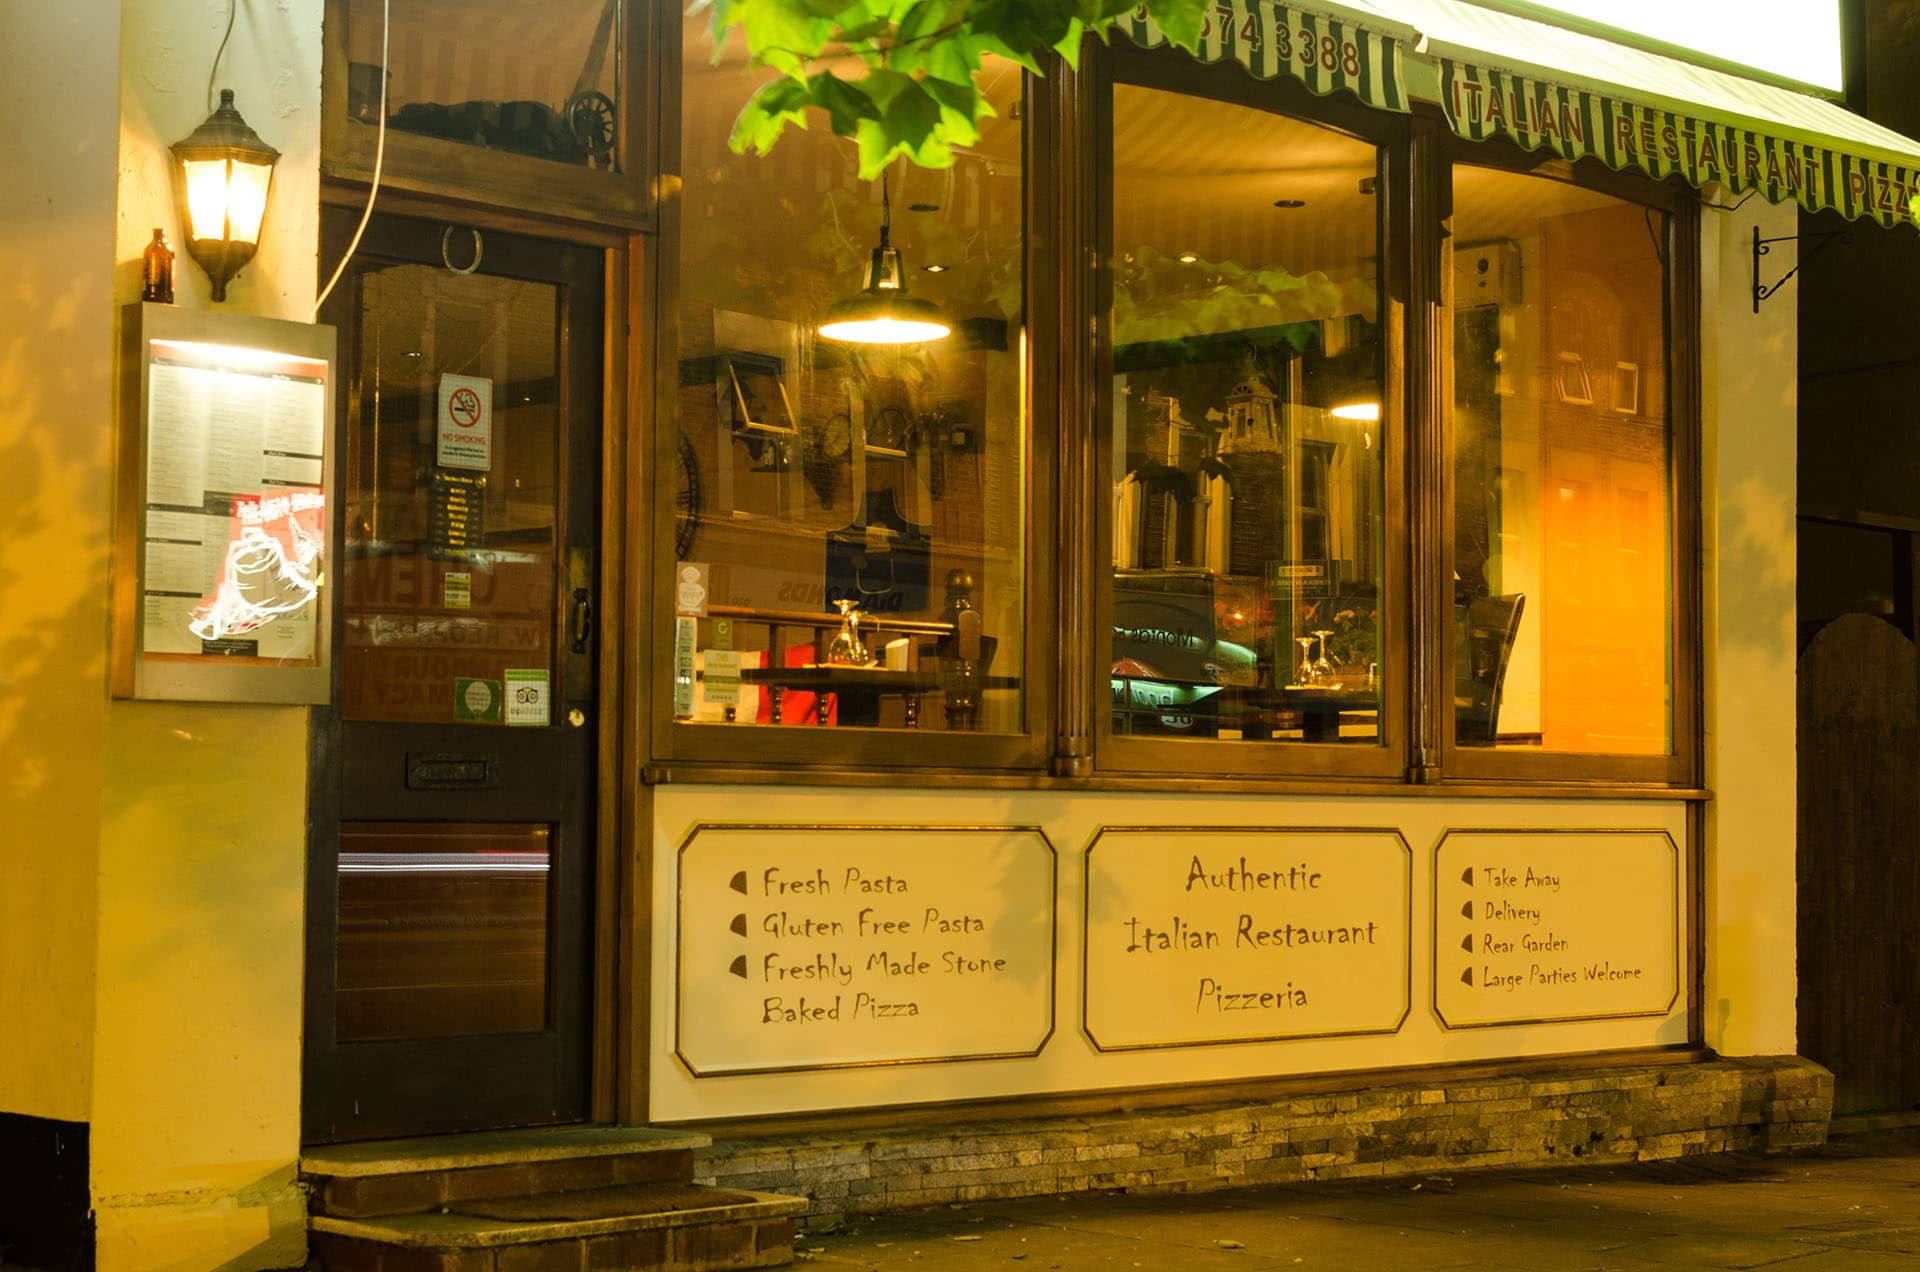
\includegraphics[width=\textwidth]{img/restaurantfront.jpg}
  \caption{Restaurace La Casa Degli Amici, foto: Martin Knapovský}
  \label{fig:restaurantfront}
\end{figure} 

\section{Marketingová strategie}

\subsection{Profil restaurace}

Tato italská restaurace vznikla na místě, kde byla do konce roku 2014 provozována italská restaurace pod jiným majitelem. Restaurace prošla částečnou renovací - do kuchyně byla nainstalována nová ventilace a plynová pec na pizzu. Vnitřní prostor restaurace nabízí 36 míst u stolů pro 2 nebo 4 lidi. K restauraci je připojena venkovní zahrádka, která pojme 42 hostů. Restaurace je umístěna v blízkosti autobusové a vlakové zastávky Tulse Hill a umožňuje rezervaci stolů pomocí telefonní objednávky. Z hlediska flexibility telefonní objednávky byla pro rezervace ponechána tato jediná možnost a možnost rezervace pomocí systému OpenTable, nebo pomocí emailu byla zamítnuta. Po telefonické objednávce poslíček restaurace doručí jídlo na smluvenou adresu. Restaurace nabízí přístup k WiFi - návštěvníci si vyžádají heslo a personál jim ho poskytne. Na březen 2017 se plánuje rozšíření restaurace o zastřešený prostor, který je nyní využíván jako venkovní zahrada.

V prostředí Londýna je vcelku běžné, že návštěvníci restaurace čekají na uvítání a usazení ke stolu. V případě, že chtějí návštěvníci jíst, je jim poskytnuto menu, olivy a pečivo. Restaurace nabízí klasické italské menu a také několik unikátních specialit, jejichž seznam se mění a je vyvěšen uvnitř restaurace. V nabídce je 18 druhů předkrmů, 17 druhů těstovin, 15 druhů pizzy, několik steaků, rybích jídel, rizota, saláty a deserty. V nabídce je také mnoho druhů italských vín a jiných alkoholických nápojů, italské nealkoholické nápoje a samozřejmě také káva a jiné teplé nápoje. Ceny jídel se pohybují v rozmezí od 5,95\pounds ~do 16\pounds.

Restaurace do doby před vytvořením facebookového (FB) profilu a webu neměla vlastní internetový obsah, který by o ní něco vypovídal.  

\subsection{Plán marketingové strategie}

Hlavním cílem strategie je vytvoření online prezentace pro posílení důvěryhodnosti a povědomí o značce za cílem navýšení zisků. Marketingová strategie je iterativní, v prvním kroku nebudeme vytvářet PR články či kupovat nové domény pro mikrostránky, které by posílily hlavní web. Zaměříme se tak na on-page SEO a propagaci na sociálních sítích. 

Kroky marketingové strategie
\begin{itemize}
	\item Zřízení domény \texttt{lacasadegliamici.co.uk}
	\item Zřízení hostingu
	\item Vytvoření propagační fotografií
	\item Vytvoření propagačního videa
	\item Vytvoření grafiky
	\item Vytvoření webu
	\item SEO optimalizace webu
	\item Vytvoření Facebook profilu
	\item Úprava Tripadvisor profilu
	\item Vytvoření Instagram profilu
	\item Provázání služeb sociálních sítí
	\item Propagace obsahu (fotografií, videí, FB)
	\item Soutěže a akční ceny
	\item Jazzové koncerty
	\item Vyhodnocení marketingové strategie
\end{itemize}

Vyhodnocení efektivnosti marketingové strategie bude provedeno na datech o tržbách zís\-ka\-ných od majitele restaurace. Vzhledem k tomu, že marketingový proces je procesem iterativním, bude na základě vyhodnocení rozhodnuto, zda bude marketingová strategie dále prohloubena o PR články a mikrostránky propagující tuto italskou kuchyni.  

\subsection{Profil zákazníka}
\label{section:customer}

Zákazník, na kterého se restaurace soustředí je typem člověka, který si rád posedí v příjemném prostředí restaurace s kvalitním jídlem za výhodnou cenu. Italská kuchyně se také vyznačuje tím, že je jídlo rychle připravené (v průměru 8 minut na jídlo) a zákazník tak může dostat jídlo velmi rychle po svém příchodu. Typický zákazník restaurace bydlí či pracuje v jejím okolí. Velmi často zákazníci přichází ve skupinách a je běžné, že je zarezervováno několik stolů k oslavě narozenin. 

\subsection{Lokální konkurence}
\label{section:competition}
V blízkém okolí restaurace se nachází indická restaurace Village Masaleh, fastfood AK Chicken, portugalská restaurace Castelo a thaiská restaurace Thaicoons. 
Village Masaleh\footnote{\url{http://www.village-masaleh.co.uk}} spustila svůj první web v září 2016 a specializuje se na dovážku jídla. Tato restaurace tak není díky rozdílnosti obchodního modelu a odlišnosti typu kuchyně přímou konkurencí.
Fastfood AK Chicken\footnote{\url{http://www.allinlondon.co.uk/directory/1165/186927.php}} je součástí širšího řetězce restaurací nabízejících smažená kuřata a hranolky. Tato restaurace není vzhledem k jejímu charakteru konkurencí - naše restaurace se zaměřujeme na zákazníka, který rád večeří v klidném prostředí s obsluhou. Tento fastfood nemá vlastní webové stránky.
Castello je portugalská kavárna s malou kuchyní bez vlastní webové prezentace. Stejně tak tomu je i u thajské restaurace Thaicoon, která vlastní doménu, avšak doména je bez obsahu\footnote{\url{http://thaicoons.com}}. 
 
Lokalitně naše restaurace získává vedoucí postavení v zisku zákazníka, na kterého se zaměřuje. Západní Norwood je z pohledu kupní síly zákazníků v porovnání se zbytkem Londýna prů\-mě\-rem - nejedná se o bohatou oblast jako centrum Londýna.\footnote{\url{http://luminocity3d.org/Economy.html\#/10/51.5241/-0.2046}}. V této oblasti se nacházejí 2 vetší vlakové zastávky - West Norwood a Tulse Hill - restaurace těží také z toho, že kolem proudí hodně lidí využívající těchto vlakových spojení. 

\begin{figure}
  \centering
    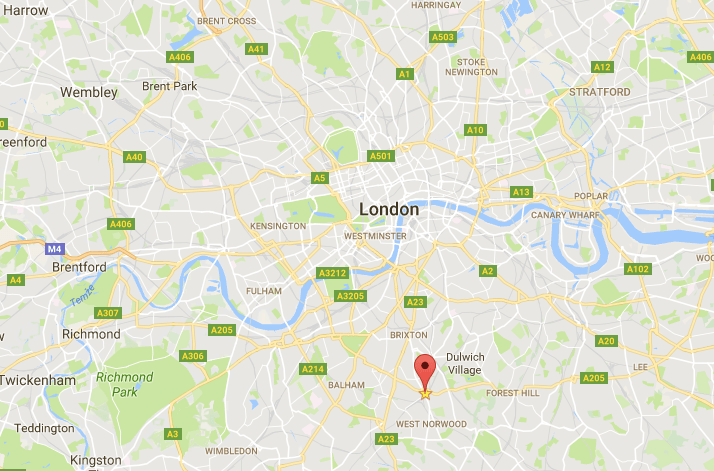
\includegraphics[width=\textwidth]{img/map.png}
  \caption{Poloha restaurace, zdroj: \url{maps.google.com}}
  \label{fig:restaurantmap}
\end{figure} 

Vzhledem k profilu restaurace a profilu jejího zákazníka, budeme propagovat:

\begin{itemize}
	\item klidnou atmosféru,
	\item možnost rezervace,
	\item možnost dovážky,
	\item snadný přístup z vlakových a autobusových zastávek,
	\item kvalitní ingredience a
	\item italskou kuchyni.
\end{itemize}

\subsection{Analýza klíčových slov}
\label{casa:kwanalysis}

K navýšení počtu zákazníků je potřeba nalákat zákazníky z širšího okolí - z tohoto důvodu volíme klíčová slova, která obsahují názvy lokalit jako Herne Hill, Brixton, Crystal Palace a další v kombinaci s řetězcem \texttt{Italian restaurant}. Předpokládá se, že největší návštěvnost restauraci přinese pokrytí řetězců \uv{Italian Restaurant Tulse Hill} a \uv{Italian Restaurant Herne Hill}. K těmto klíčovým slovům, která vložíme do \texttt{<title>} a \texttt{<h1>} tagů přidáme také klíčová slova popisují restauraci tak, jak jsme si to uvedli v předchozí kapitole. Tato dodatečná klíčová slova budou obsažena v obsahovém bloku stránky.  

K analýze klíčových slov byl použit nástroj Moz Keyword Explorer. Tento nástroj byl použit pro analýzu pokrytí různých klíčových slov, které jsme si vybrali:

\begin{itemize}
	\item Italian Restaurant
	\item Tulse Hill
	\item Herne Hill
	\item Crystal Palace
	\item Delivery
	\item Quality Ingredience
	\item Quality Food
	\item Italian Cuisine
	\item ...
\end{itemize}

Na obrázcích \ref{fig:moz1}, \ref{fig:moz2} a \ref{fig:moz3} je ukázána kombinace slov \uv{Italian Restaurant Tulse Hill}, \uv{Italian Restaurant Herne Hill} a \uv{Italian Restaurant London}. Nástroj ohodnocuje kombinaci \uv{Italian Restaurant London} jako kombinaci s větším potenciálem a větší náročností. Vzhledem k tomu, že se soustředíme na lokální zákazníky, používáme klíčová slova popisující obsahující názvy okolních lokalit - tato klíčová slova jsou vzhledem k cíli marketingové strategie naší restaurace vhodnější a mělo by být snažší v pokrytí těchto klíčových slov uspět. Na obrázcích je také možné vidět, že kombinace klíčových slov s lokálními názvy jsou tak málo pokryté, že o nich neexistují data v databázi \url{https://moz.com/explorer/}.  


\begin{figure}
  \centering
    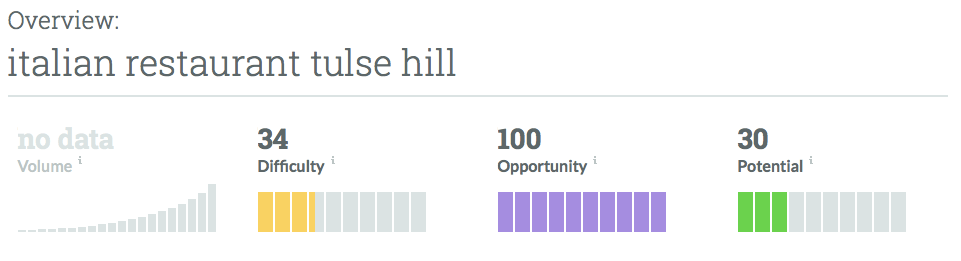
\includegraphics[width=\textwidth]{img/moz1.png}
  \caption{Analýza kombinace klíčových slov \uv{italian restaurant tulse hill}, zdroj: \url{https://moz.com/explorer/}}
  \label{fig:moz1}
\end{figure} 


\begin{figure}
  \centering
    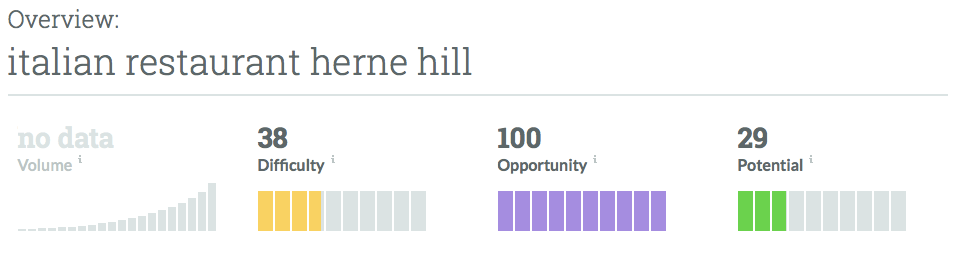
\includegraphics[width=\textwidth]{img/moz2.png}
  \caption{Analýza kombinace klíčových slov \uv{italian restaurant herne hill}, zdroj: \url{https://moz.com/explorer/}}
  \label{fig:moz2}
\end{figure} 


\begin{figure}
  \centering
    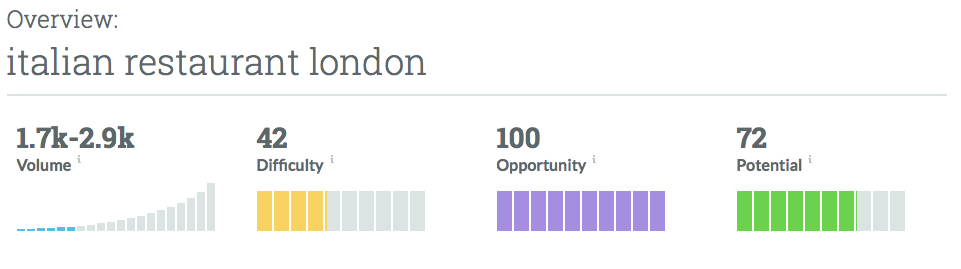
\includegraphics[width=\textwidth]{img/moz3.png}
  \caption{Analýza kombinace klíčových slov \uv{italian restaurant london}, zdroj: \url{https://moz.com/explorer/}}
  \label{fig:moz3}
\end{figure} 


V následující části práce bude ve stručnosti zmíněna implementace jednotlivých bodů marketingové strategie, větší prostor bude poskytnut samotné optimalizaci pro vyhledávače, na kterou se tato práce zaměřuje.

\section{Vytvoření propagačních fotografií a videa}

Fotografie použité na webu byly foceny přímo v restauraci za běžného provozu. Bylo nutné nafotit jídla od každé kategorie, aby následně bylo možné pomocí těchto fotografií oddělit jednotlivé části menu. Dalším nutným krokem bylo nafotit vnitřní a venkovní prostory restaurace - vstup, restauraci samotnou a venkovní zahrádku. Použité fotografie se nacházejí na přiloženém CD. K pořízení fotografií byl použit fotoaparát Nikon D5100 s objektivem Nikon 35mm f/1,8G AF-S DX. 
 
 \begin{figure}
  \centering
    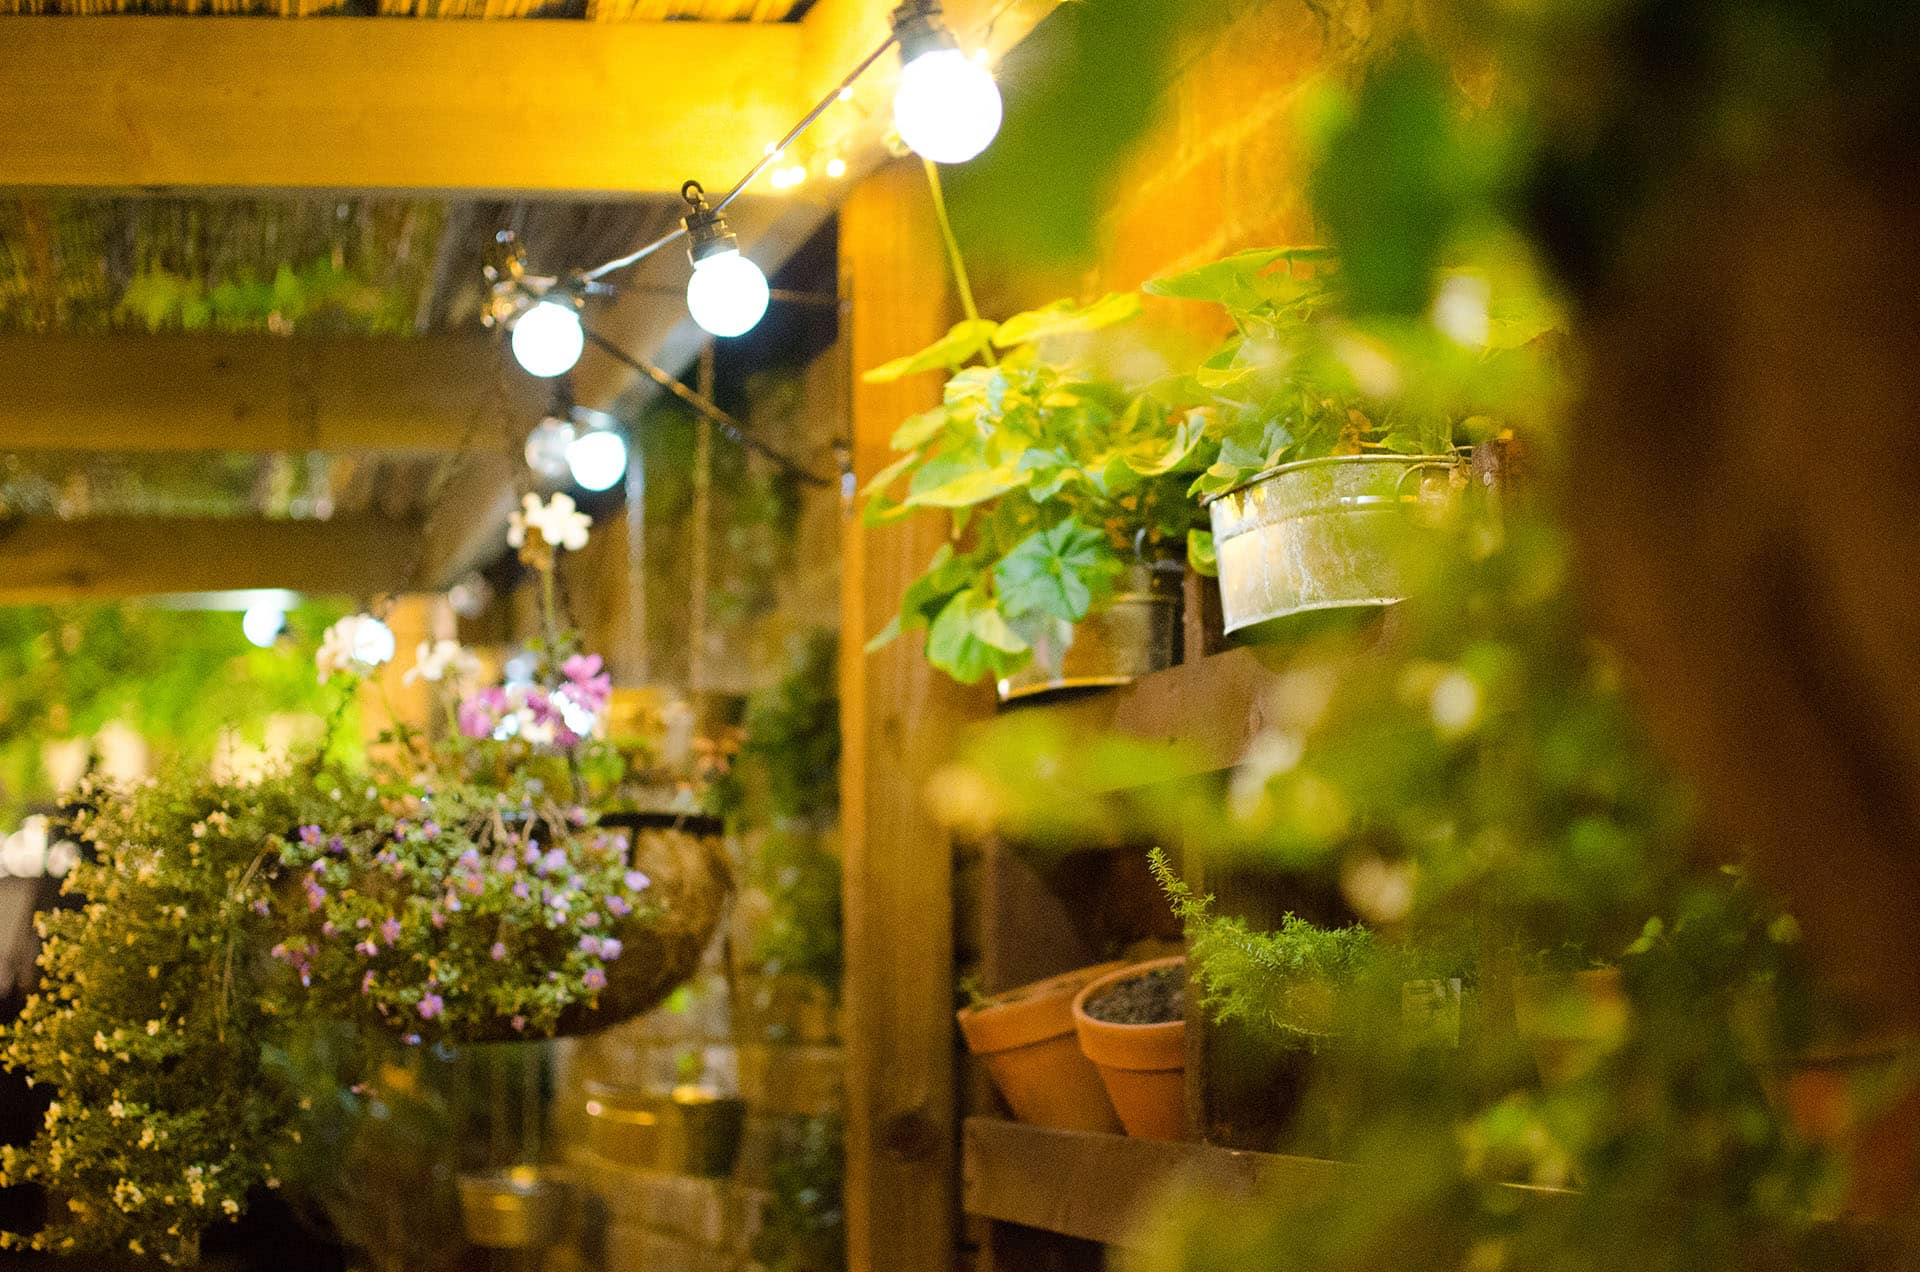
\includegraphics[width=\textwidth]{img/garden.jpg}
  \caption{Ukázková fotografie restaurace, autor: Martin Knapovský}
  \label{fig:garden}
\end{figure} 

Pro restauraci bylo také pořízeno krátké video prezentující jeden z jazzových koncertů. Cílem videa bylo přiblížit návštěvníkům webových stránek atmosféru restaurace a také nahlédnout do zákulisí kuchyně. Video je umístěno na serveru Youtube\footnote{\url{https://www.youtube.com/watch?v=TXiv5hCqXK0}}.

\newpage
\section{Vývoj webu}

\subsection{Zřízení domény}

Doména \url{lacasadegliamici.co.uk} byla zřízena u registrátora \url{names.co.uk} a byla pře\-smě\-ro\-vá\-na na server, na kterém jsou umístěny webové stránky restaurace. \uv{Nameservery} byly nastaveny takto:

\begin{itemize}
	\item NS1: \texttt{ns1.contabo.net (79.143.182.242, 2a02:c200:0:10::882:1)}
	\item NS2: \texttt{ns2.contabo.net (178.238.234.231, 2a02:c200:0:10::891:1)}
	\item NS3: \texttt{ns3.contabo.net (5.189.191.29, 2a02:c200:1:10::842:1)}
\end{itemize}

DNS zóna je spravována na serverech \texttt{contabo.net}.

\subsection{Zřízení hostingu}

Webové stránky jsou hostovány na VPS serveru společnosti Contabo\footnote{\url{https://contabo.com}} s konfigurací \texttt{Intel(R) Xeon(R) CPU E5\-2620 v3 @ 2.40GHz, 4 cores}, \texttt{12GB RAM}, \texttt{300GB SSD}. Na serveru je nainstalován \texttt{Ubuntu Linux 16.04.1}, \texttt{Linux 4.4.0-34-generic, x86\_64} s konfiguračními panely \texttt{Webmin 1.810}, a \texttt{Virtualmin 5.04}\footnote{URL adresa serveru: \url{vmi82405.contabo.host}}. Web \texttt{lacasadegliamici.co.uk} má vytvořen svůj vlastní hosting s diskovou kvótou 10GB. Hosting obsahuje obsahuje firewall, AWstats statistiky, mailové adresy s filtrací spamu, FTP účet, MySQL databáze a uživatelský účet pro přihlášení do konfiguračního rozhraní. Je použit server Apache 2.4.18 s PHP 7.0 a databází MySQL 5.7.15. Kompletní \texttt{phpinfo()} je dostupné na přiloženém CD.

VPS server byl použit z důvodu možnosti pokročilého nastavení serveru - základní sdílený hosting často neumožňuje měnit maximální velikost nahrávaných souborů, změnu \textit{PHP timeoutu}, cachování a další důležitá nastavení, která můžeme využít pro urychlení webových stránek a minimalizaci jejich datové velikosti.

\subsection{Volba redakčního systému}

Web byl postaven na open-source redakčním systému Wordpress\footnote{\url{https://wordpress.org}}, který je napsaný v PHP a MySQL a je vyvíjený pod licencí GNU GPL. Tento redakční systém byl vybrán z důvodu jeho široké uživalské a vývojářské komunity a kvůli velkému množství dostupných pluginů, které urychlují vývoj webu. Wordpress je dle statistik\footnote{\url{https://w3techs.com/technologies/overview/content_management/all}} používán jako redakční systém na více než 25 \% webových stránek na světě. Počet stažení verze 4.4 samotné dosahovalo po 14 dnech od vydání téměř 5,5 milionu\footnote{\url{https://wordpress.org/download/counter/}}. Dalšími často používanými redakčními systémy jsou Joomla\footnote{\url{https://www.joomla.org}} či Drupal\footnote{\url{https://www.drupal.org}} - ty se však v používanosti drží kolem tří procent. 

 \begin{figure}
  \centering
    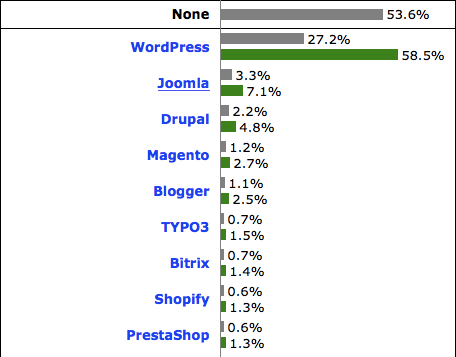
\includegraphics[width=\textwidth]{img/wordpressusage.png}
  \caption{Wordpress jako nejpoužívanější redakční systém, zdroj: W3Techs.com, 26. 11. 2016}
  \label{fig:wordpressusage}
\end{figure} 

Mezi redakčními systémy Wordpress získává téměř šedesátiprocentní část trhu (obrázek \ref{fig:wordpressusage}). Mezi základní vlastnosti Wordpressu patří:
\begin{itemize}
	\item systém má otevřený zdrojový kód, který je dostupný zdarma a kdokoliv ho může upravit
	\item Wordpress dodržuje standardy XML, XHTML a CSS
	\item systém má integrovaného správce odkazů
	\item integrovaná galerie médií (správa obrázků a jejich základní editace přímo v redakčním systému, automatické vytváření miniatur definovaných rozměrů)
	\item kvalitní podpora SEO s množstvím uživatelských nastavení - např. možnost nastavení struktury odkazů
	\item podpora pluginů pro rozšíření funkcí - v oficiálním repozitáři je jich k dispozici téměř 50 000
	\item podpora témat vzhledu
	\item podpora funkčních bloků - tzv. widgetů (např. poslední příspěvky, vlastní text, výpis RSS, atd.)
	\item možnost zařazovat příspěvky do kategorií (i do více najednou)
	\item možnost přidávat příspěvkům štítky (tagy) pro zlepšení navigace
	\item lze vytvářet hierarchii (strom) stránek
	\item podpora pro trackback a pingback (automatické odeslání informace o novém obsahu externím službám a přijetí tohoto upozornění, pokud na stránky někdo jiný odkáže)
	\item podpora vkládání externího obsahu pomocí formátu oEmbed
	\item podpora více uživatelských účtů s odlišnými oprávněními
\end{itemize}

Pro stavbu webu \url{lacasadegliamici.co.uk} byla použivata verze \texttt{Wordpress 4.5.3}, která vyšla 21. června 2016. 

\subsection{Šablona webu}

Jak již bylo napsáno v popisu systému Wordpress, tento systém podporuje šablony, pomocí kterých je možné nastavit vzhled webu. Vzhled by měl být lákavý, aby zaujmuj uživatele a společně s kvalitním obsahem ho udržel na stránkách. Po konzultaci s majitelem restaurace byla použita šablona ROSA\footnote{\url{https://themeforest.net/item/rosa-an-exquisite-restaurant-wordpress-theme/7920093}}, která posloužila jako dobrý základ pro vývoj webu. Šablona byla upravována přepisováním souborů v tzv. \texttt{child-theme}, což je podšablona, která obsahuje pouze upravené soubory a ty, které v ní nejsou obsaženy, načítá z původní šablony. Pomocí této dědičnosti je tak možné aktualizovat originální šablonu a v  podšabloně zachovávat úpravy. Šablona je rovněž připravená pro eCommerce řešení WooCommerce\footnote{\url{https://woocommerce.com}}, díky kterému lze v budoucnu webovou prezentaci restaurace přeměnit na internetový obchod pro rozvážku jídla. 

\subsection{Použité pluginy}

Pluginy slouží k rozšíření základní funkcionality Wordpressu. Může se jednat o plugin pro výpis zákaznického hodnocení, kalendář s možností rezervace, nebo například plugin pro práci s databází. Díky početné komunitě, která Wordpress obklopuje, můžeme najít velké množství pluginů. Následuje seznam a stručný popis jednotlivých Wordpress pluginů, které byly použity pro vývoj webu a pro následnou SEO optimalizaci.

\begin{itemize}
	\item \textbf{Contact Form 7}\footnote{\url{https://wordpress.org/plugins/contact-form-7/}} - Plugin, který umoňuje tvorbu jednoduchých kontaktních formulářů pomocí tzv. \uv{shortcodes} 
	\item \textbf{Pixcodes}\footnote{\url{https://wordpress.org/plugins/pixcodes/}} - Tento plugin umožňuje použivání shortcodes pro tvorbu sloupců a pro vkládání různého druhu obsahu - galerie, videa, tlačítka, ...
	\item \textbf{W3 Total Cache}\footnote{\url{https://wordpress.org/plugins/w3-total-cache/}} - Alternativa k Google PageSpeed Apache modulu, která nabízí uživatelské nastavení cache, minifikace souborů, cache prohlížeče, CDN a dalších prvků, které lze použít k urychlení webových stránek (viz kapitola \ref{section:datasizeoptimalization}).
	\item \textbf{WP Smush}\footnote{\url{https://wordpress.org/plugins/wp-smushit/}} - Plugin, který umožňuje nahrávání nových obrázků do Wordpress systému s jejich automatickou optimalizací
	\item \textbf{Yoast SEO}\footnote{\url{https://wordpress.org/plugins/wordpress-seo/}} - Plugin určený k on-page SEO, tvorbě XML sitemap, práci s Google Webmaster Tools atd.  
\end{itemize}

\newpage
\subsection{Struktura webu}

Struktura a obsah webu odpovídá bodům, které jsme si vytyčili v kapitole \ref{section:competition}. Propagujeme klidnou atmosféru, možnost rezervace, dovážky, snadný přístup z autobusových a vlakových stanic, kvalitní ingredience a italskou kuchyni. Web obsahuje 9 základních stránek a 10 podstránek menu. Následuje jejich seznam a stručný popis:

\begin{itemize}
	\item Domovská stránka
	\item Menu
		\begin{itemize}
			\item Předkrmy
			\item Těstoviny
			\item Rizoto
			\item Velké saláty
			\item Přílohy
			\item Ryby
			\item Steaky
			\item Omáčky
			\item Pizza
			\item Dezerty
		\end{itemize}
	\item Rezervace
	\item Lokace
	\item Kontakt
	\item Podmínky použítí
	\item DMCA
	\item Zásady ochrany osobních údajů
	\item XML sitemapa
\end{itemize}  

\subsubsection{Hlavička a patička webu}

Hlavička webu obsahuje \textbf{menu} s odkazy na domovskou stránku, menu, rezervace, lokaci a kontakt. Při najetí na odkaz v menu, vyjíždí nabídka pro podstránky jednotlivých typů jídel. Uživatel tak nemusí listovat celým menu a může ihned přejít na sekci, která ho zajímá. Hlavička je k vidění na obrázku \ref{fig:lacasasample}.

Patička webu je na obrázku \ref{fig:footer}. Patička obsahuje odkazy na sociální sítě, na kterých jsou zveřejňovány výhodné nabídky, adresu restaurace, telefonní číslo do restaurace, odkazy na podmínky použití, DMCA a zásady ochrany osobních údajů, odkaz na sitemapu a na stránky autora webu\footnote{\url{https://www.knapovsky.com}}. Pomocí dvojitých šipek se lze po kliknutí dostat zpět na horní část aktuálně zobrazené stránky. Odstraňuje se tak nutnost \uv{scrollovat} přes celou stránku.

 \begin{figure}
  \centering
    
\includegraphics[width=\textwidth]{img/footer.png}
  \caption{Vzhled webu - patička, zdroj: \url{lacasadegliamici.co.uk}, 26. 11. 2016}
  \label{fig:footer}
\end{figure} 

\subsubsection{Domovká stránka}

Domovská stránka obsahuje několik podsekcí, které jsou odděleny tzv. \uv{parallax obrázkem} - obrázek se při pohybu stránky pohybuje jinou rychlostí než zbytek stránky a vzniká tak lákavý prostorový efekt. 

 \begin{figure}
  \centering
    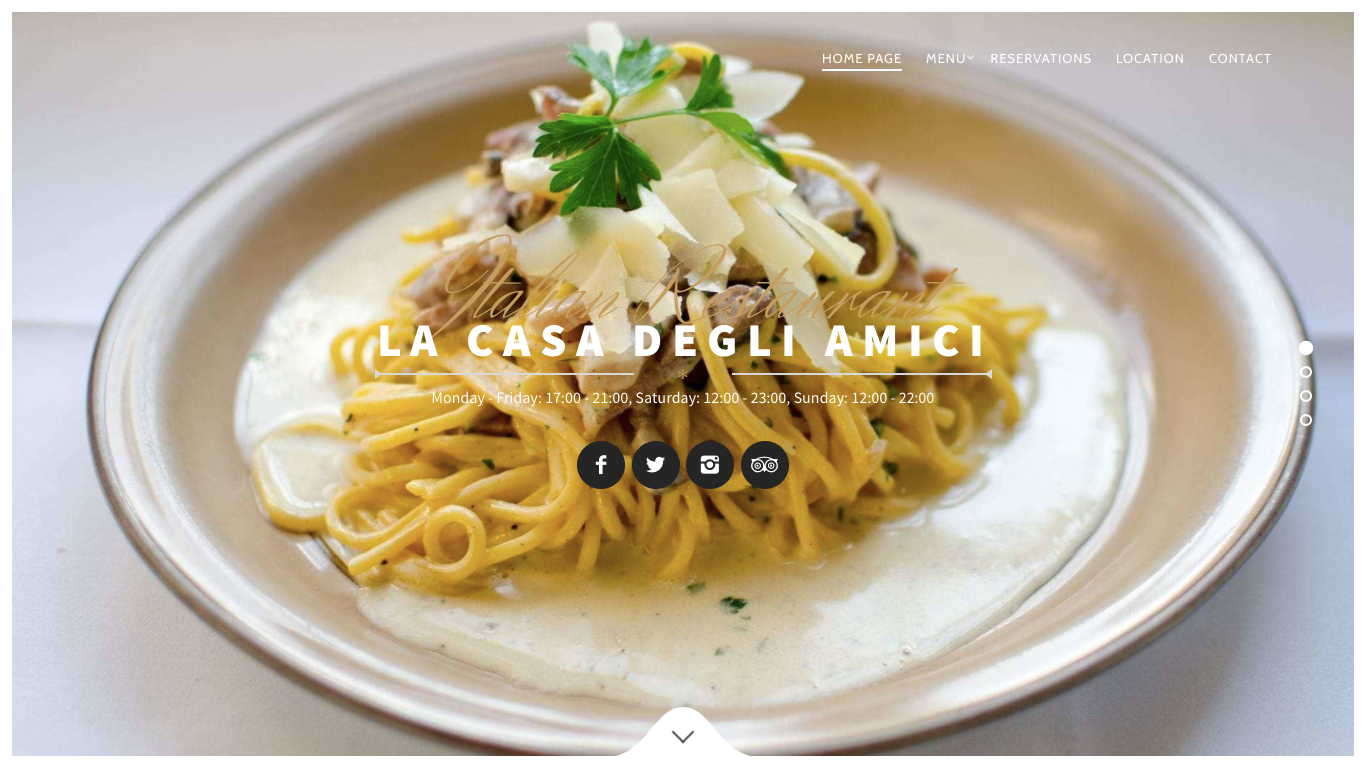
\includegraphics[width=\textwidth]{img/lacasasample.png}
  \caption{Vzhled domovské stránky webu, zdroj: \url{lacasadegliamici.co.uk}, 26. 11. 2016}
  \label{fig:lacasasample}
\end{figure} 

Horní část domovské stránky jsme si ukázali na obrázku \ref{fig:lacasasample}. Při načtení stránky je uživateli prezentována fotografie jídla z restaurace, otevírací doba restaurace a odkazy na sociální sítě - Facebook, Twitter, Instagram a Tripadvisor. V pravé části stránky se zobrazují 4 tečky, které slouží k posunu mezi jednotlivými částmi domovské stránky. Jednotlivé části domovské stránky ve stručnosti popisují restauraci a směrují uživatele na podstránky pro rezervaci, menu a opět na sociální sítě.

 \begin{figure}
  \centering
    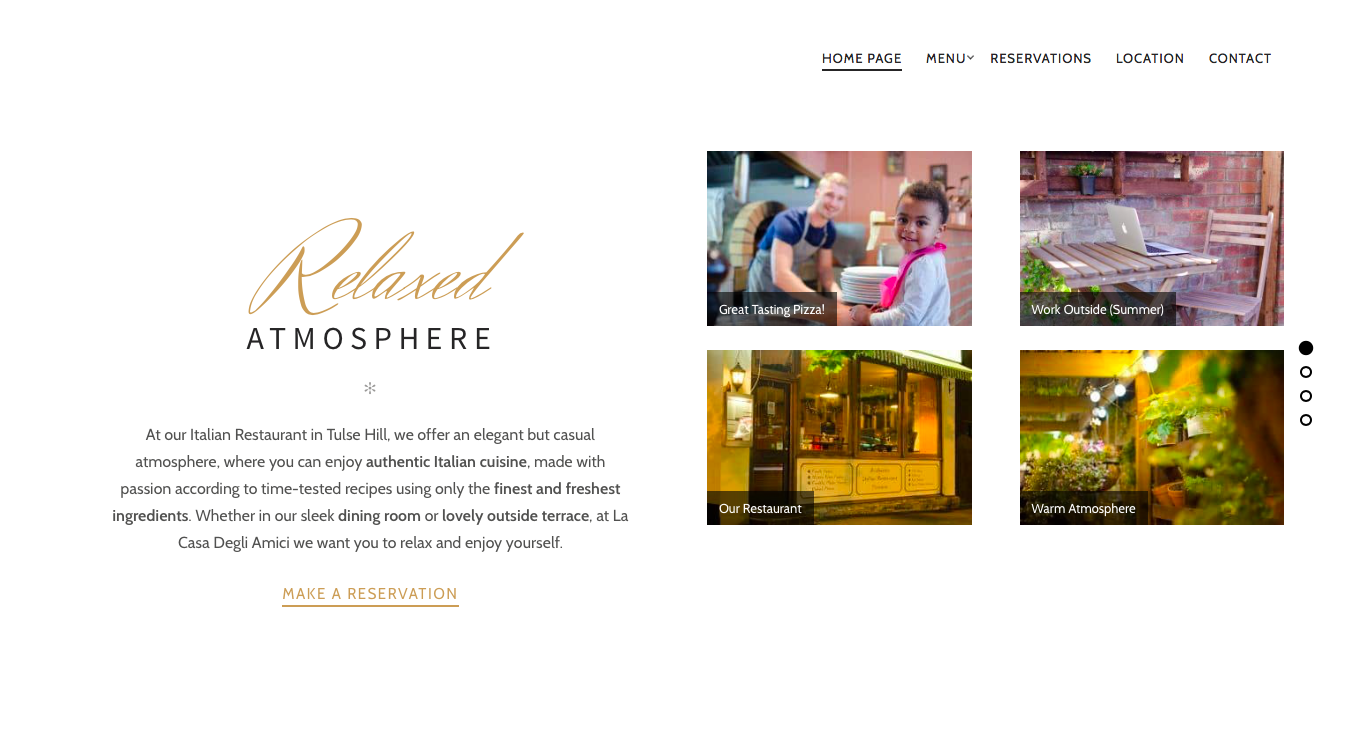
\includegraphics[width=\textwidth]{img/lacasarelaxed.png}
  \caption{Vzhled domovské stránky webu - základní info, zdroj: \url{lacasadegliamici.co.uk}, 26. 11. 2016}
  \label{fig:lacasarelaxed}
\end{figure} 

Na obrázku \ref{fig:lacasarelaxed} je vyobrazena další část domovské stránky, která stručně popisuje prostory a atmosféru restaurace. Pro lepší představu je popis doplněn fotografiemi v pravé části. Na obrázku je také možné si povšimnout, že menu se podbarvilo na bílou barvou a posunulo se spolu s tím, jak se uživatel posunul ve stránce. Uživateli je tak menu stále dostupné a může rychle přejít mezi jednotlivými stránkami webu. 

Následuje povídání o menu restaurace, o specialitách, ingrediencích a odkaz na kompletní menu (obrázek \ref{fig:lacasahomemenu}). Na předchozím i tomto obrázku je možné vidět volbu klíčových slov tak, aby odpovídaly předchozí analýze (kapitola \ref{casa:kwanalysis}) a zároveň věrně popisovaly restauraci.  

 \begin{figure}
  \centering
    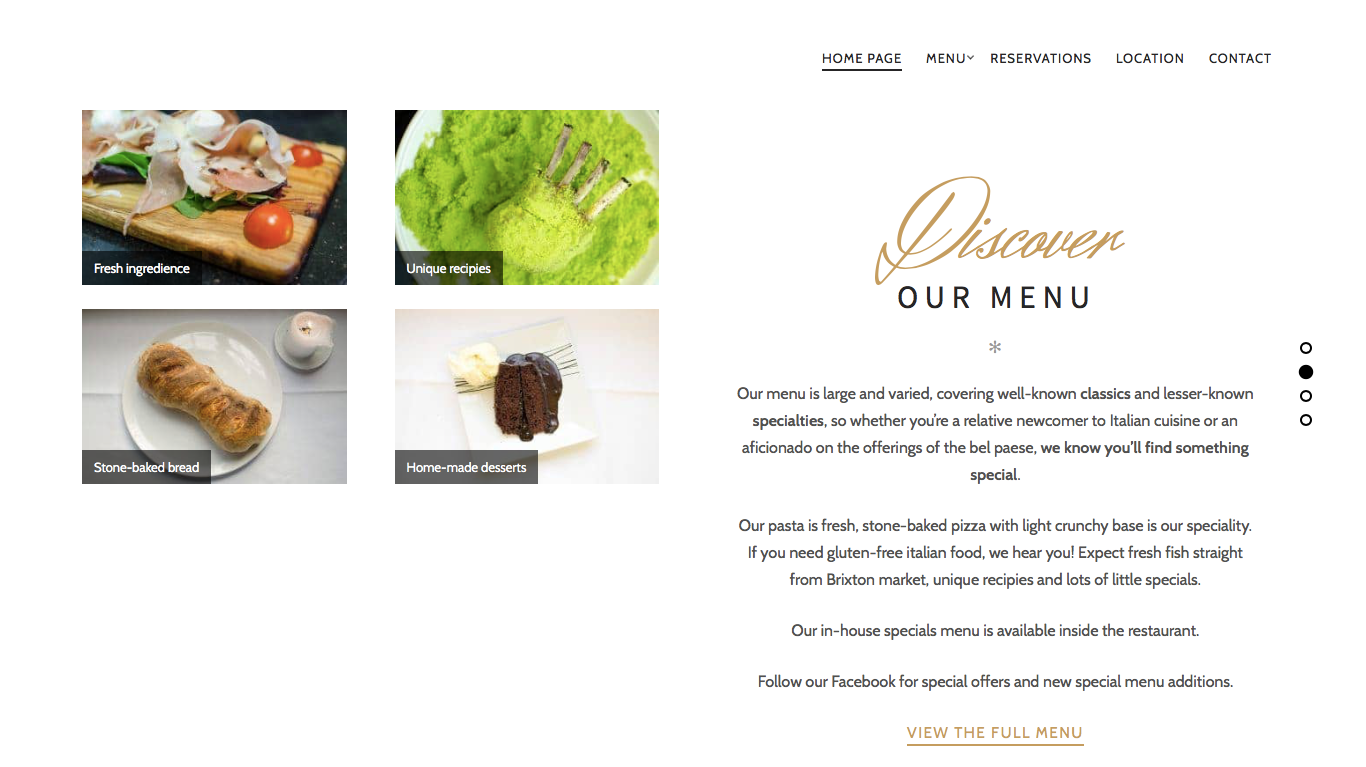
\includegraphics[width=\textwidth]{img/lacasahomemenu.png}
  \caption{Vzhled domovské stránky webu - popis menu, zdroj: \url{lacasadegliamici.co.uk}, 26. 11. 2016}
  \label{fig:lacasahomemenu}
\end{figure} 

Dále na domovské stránce nalezneme odkaz na recenze z TripAdvisoru a odkaz na video z restaurace. Video ve dvou a půl minutách přibližuje atmosféru restaurace při jazzovém koncertu z 2. 7. 2016. Video je velmi dobrým popisným prostředkem, který uživateli dobře přiblíží prostory restaurace a také proces pečení pizzy a vaření těstovin\footnote{video dostupné z \url{https://www.youtube.com/watch?time_continue=2&v=TXiv5hCqXK0}}. Video je také součástí přílohy diplomové práce.

Následuje část stránky (obrázek \ref{fig:delivery}), která nabízí dovážku do míst v jihovýchodního a jihozápadního Londýna. Text obsahuje názvy jednotlivých lokalit v kombinaci s jejich poštovními kódy, které jsou v rámci Londýna často používané k lokalizaci domů a podniků. Volba tohoto textu plyne ze skutečnosti popisované v marketingové strategii - snažíme se nalákat lidi z okolí restaurace a používáme k tomu názvy okolních lokalit v kombinaci s názvem restaurace a dalšími klíčovými slovy obsaženými v textu. 

 \begin{figure}
  \centering
    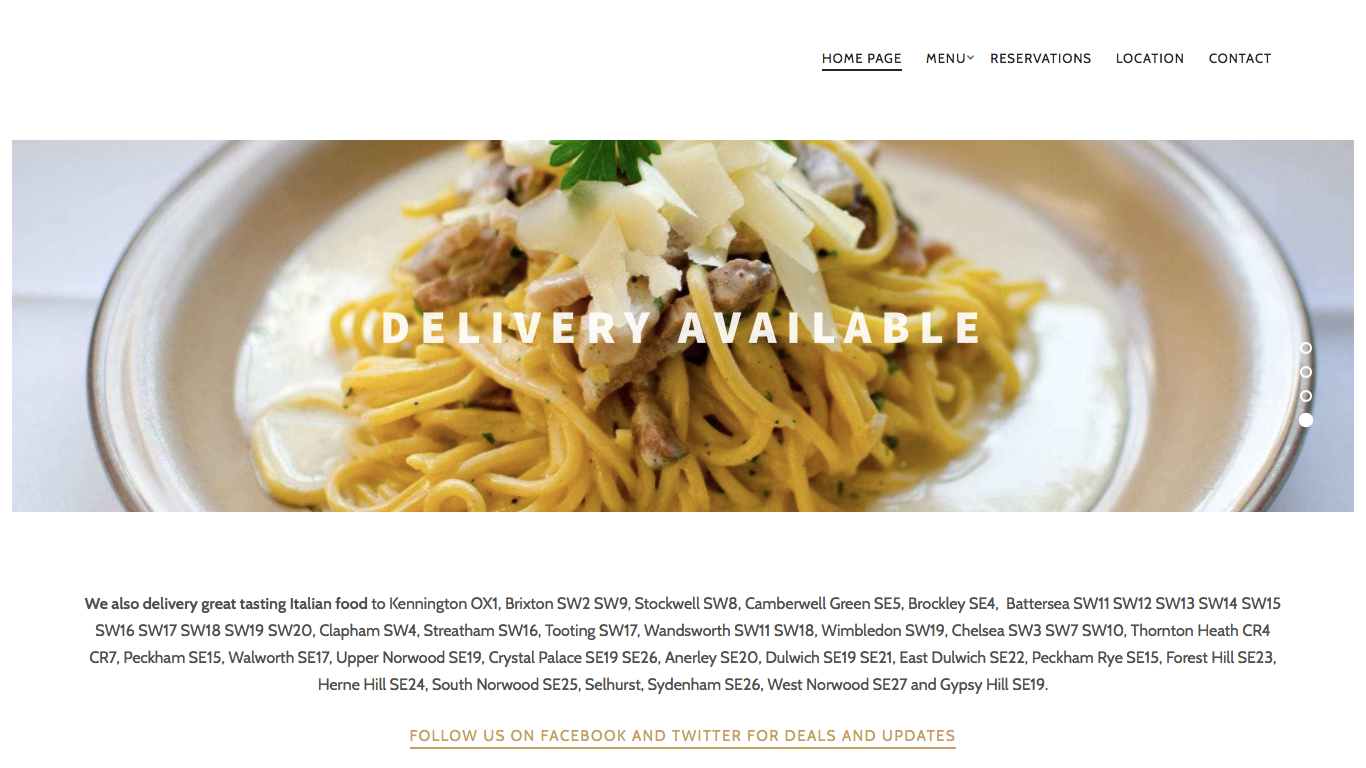
\includegraphics[width=\textwidth]{img/delivery.png}
  \caption{Vzhled domovské stránky webu - část nabízející dovážku, zdroj: \url{lacasadegliamici.co.uk}, 26. 11. 2016}
  \label{fig:delivery}
\end{figure} 

\subsubsection{Menu}
\label{casa:menu}

Menu obsahuje mnoho obrázků s parallax efektem, který by měl zaměřit pozornost uživatele na samotný obrázek a nalákat ho tak k objednání jídla, nebo k návštěve restaurace. Každý typ jídla má svou sekci, ke které je možné se rychle dostat pomocí odkazu v hlavičce, nebo pomocí JavaScriptové navigace v pravé části obrazovky. Menu v úvodním textu vyzdvihuje kvality kuchyně a nabízí výhodné menu. 

Každé jídlo má svůj italský název (přání majitele restaurace), popis jídla a soupis ingrediencí. V menu jsou uvedeny klasická jídla této restaurace, seznam specialit je často měněn a je tedy uveden v restauraci a propagován pomocí sociálních sítí. Ukázka menu je na obrázku \ref{fig:menu}.

 \begin{figure}
  \centering
    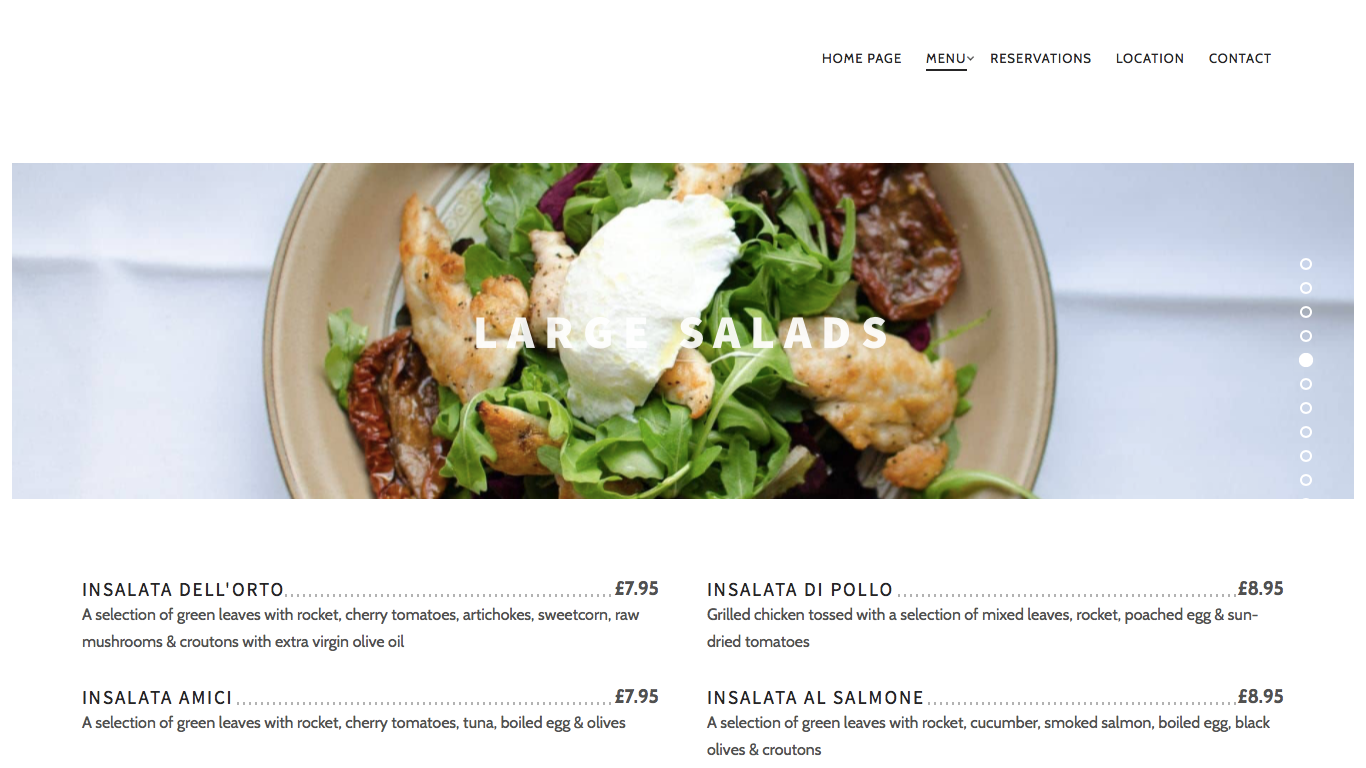
\includegraphics[width=\textwidth]{img/menu.png}
  \caption{Vzhled menu, zdroj: \url{lacasadegliamici.co.uk}, 26. 11. 2016}
  \label{fig:menu}
\end{figure} 

\subsubsection{Rezervace}

Jak bylo uvedeno v profilu restaurace, rezervace a objednávky probíhají telefonicky a není tedy potřeba vytvářet či navazovat další systém, který by rezervace a objednávky spravoval. Stránka rezervace obsahuje počet dostupných míst a prostorů k rezervaci, jejich fotografie a postup rezervace. 

\subsubsection{Lokace}

Lokační stránka obsahuje interaktivní mapu s polohou restaurace a trasu od nejbližších autobusových a vlakových stanic. Pro lepší orientaci je zde také vložena fotografie restaurace. 

\subsubsection{Kontakt}

Kontaktní stránka obsahuje konktní formulář, jehož obsah je odeslán majiteli restaurace. Ukázka formuláře je na obrázku \ref{fig:form}.

 \begin{figure}
  \centering
    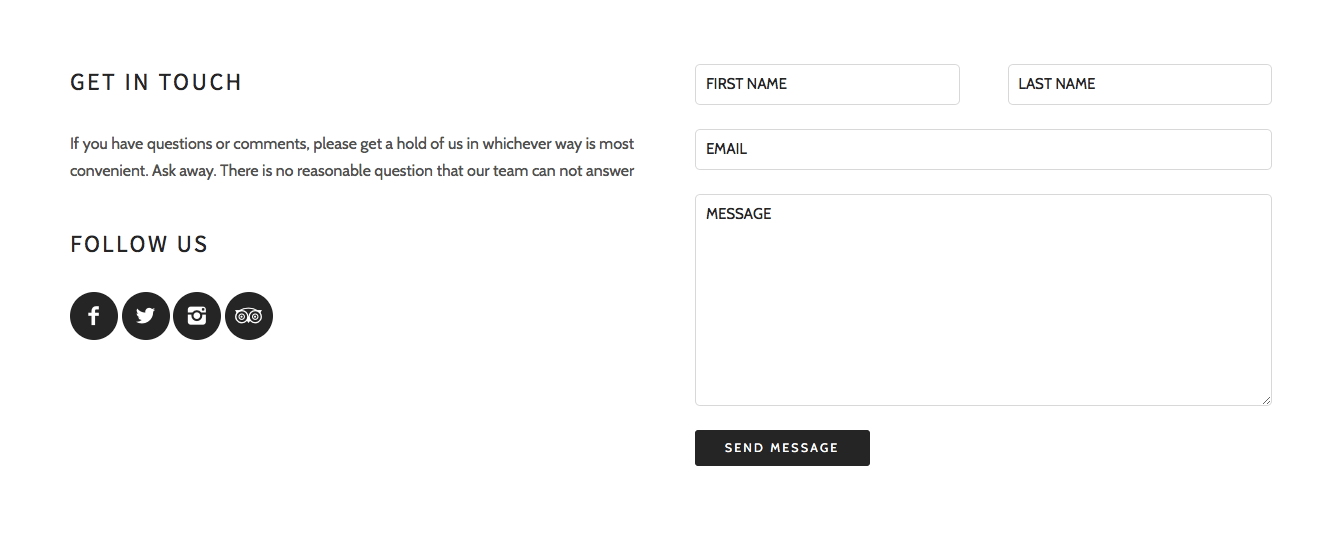
\includegraphics[width=\textwidth]{img/form.png}
  \caption{Vzhled kontaktního formuláře, zdroj: \url{lacasadegliamici.co.uk}, 26. 11. 2016}
  \label{fig:form}
\end{figure} 

\subsubsection{Podmínky použití a další stránky}

Podmínky použití obsahují právní podmínky k použití webových stránek \texttt{lacasadegliamici.\-co.\-uk}, DCMA neboli \textbf{D}igital \textbf{M}illenium \textbf{C}opyright \textbf{A}ct stránka ustanovuje podmínky pro zacházení s autorským obsahem na webových stránkách a také způsoby pro nahlášení nelegálně publikovaného obsahu. Zásady ochrany osobních údajů uvádějí jakým způsobem je zacházeno s osobními údaji uživatelů. Tyto 3 stránky jsou důležité pro vyhledávač Google, který přítomnost těchto stránek na webu zohledňuje při ohodnocení stránky\footnote{\url{http://backlinko.com/google-ranking-factors\#}}. 

\subsubsection{XML sitemapa}

Na webu je také dostupná XML sitemmapa, která obsahuje strukturu webu včetně provázání jeho jednotlivých stránek a bude použita pro indexaci nástrojem Google Webmaster Tools. 

\section{Aplikace vybraných SEO technik}

V této části práce si projdeme způsob, kterým byl optimalizovaný web \texttt{lacasa\-degli\-amici\-.co\-.uk}. Budeme se často odkazovat na kapitolu \ref{section:SEO}, která položila teoretické základy nutné k pochopení souvislostí mezi informacemi, které budou následovat. 

\subsection{On-Page SEO}

Pro on-page optimalizaci byl použit Wordpress plugin Yoast SEO, který umožňuje optimalizovat titulky a meta popisky jednotlivých stránek, umožňuje jednoduché propojení s Google Webmaster Tools a umožňuje generovat XML sitemapy, které se pak do Webmaster Tools nahrávají.  

Yoast SEO plugin umožňuje ohodnocení kvality optimalizace přímo v adminstraci webových stránek. Každá ze stránek webu byla upravena tak, aby titulek obsahoval název stránky (Menu, Reservation, ...) a telefonní číslo pro rychlou objednávku. Délka titulku se pohybuje kolem 55 znaků. Hodnocení, které plugin provádí je určeno pro obsah, který neobsahuje shortcodes a také není určen pro stránky, jejichž obsah se skládá z více wordpressových podstránek - tak je tomu například u domovské stránky a jídelního menu. Jak je možné vidět na obrázku \ref{fig:yoast}, plugin si stěžuje na krátký text a vynechání \texttt{<h2>} HTML tagu, který by obsahoval klíčové slovo \uv{italian}. Pokud však načteme celou stránku, kterou takto plugin ohodnotil (domovská stránka), zjistíme, že klíčové slovo je obsaženo poměrně často a že text domovské stránky obsahuje 332 slov, což je více než plugin pro dobré ohodnocení požaduje. 

\begin{figure}
  \centering
    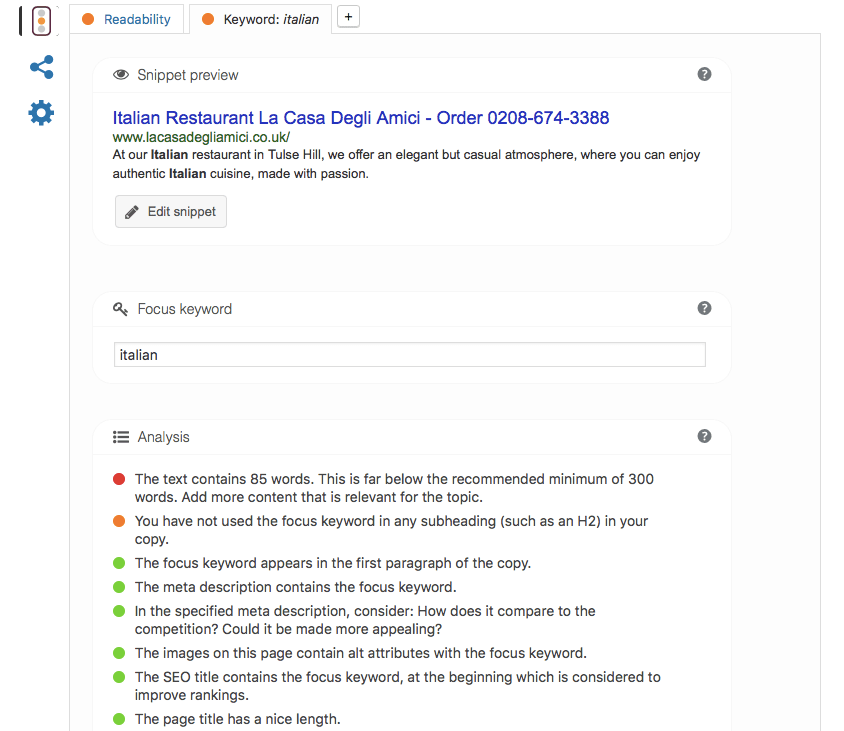
\includegraphics[width=\textwidth]{img/yoast.png}
  \caption{Optimalizační plugin Yoast SEO, zdroj: \url{lacasadegliamici.co.uk}, 26. 11. 2016}
  \label{fig:yoast}
\end{figure} 

\subsubsection{Komprimace přenášených dat}

Použitý server Apache byl nastaven tak, aby komprimoval přenášená data pomocí gzip komprimace. Komprimuje se HTML stránka, CSS i JS. U samotného HTML souboru domovské stránky bylo uspořeno více než 40kB s efektivností komprimace 78,9 \%.

 \begin{figure}
  \centering
    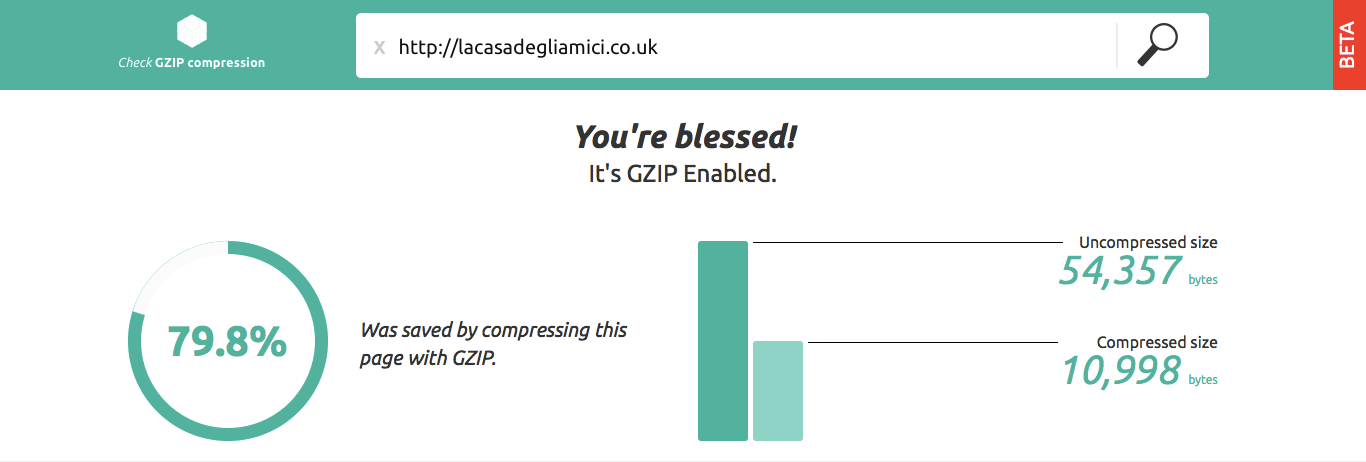
\includegraphics[width=\textwidth]{img/gzip.png}
  \caption{Úspora vzniklá zapnutím \texttt{gzip} komprese, zdroj: \url{checkgzipcompression.com}, 26. 11. 2016}
  \label{fig:gzip}
\end{figure} 

\subsubsection{Minifikace souborů a CDN}
\label{section:minifycdn}

HTML soubory byly minifikovány pomocí HTML Tidy\footnote{\url{http://www.html-tidy.org}}, JavaScript pomocí JSMin\footnote{\url{http://crockford.com/javascript/jsmin}} a CSS pomocí YUI compressor\footnote{\url{http://yui.github.io/yuicompressor/}}. CSS styly jsou spojeny do jednoho souboru, takže prohlížeč při načítání stylů nemusí posílat více HTTP dotazů.

CSS soubory, který byly spojeny:
\begin{itemize}
	\item wp-content/plugins/contact-form-7/includes/css/styles.css - Styl pluginu pro tvorbu formulářů - 1,24kB
	\item wp-content/plugins/pixlikes/css/public.css - Styl pluginu pixlikes
	\item wp-content/themes/rosa/style.css - Styl šablony ROSA - 337kB
	\item wp-content/themes/rosa-child/style.css - Styl dceřinné šablony ROSA - 2kB
	\item wp-content/plugins/jetpack/css/jetpack.css - Styl pluginu Jetpack - 60kB
\end{itemize}

Výsledný minifikovaný a zkombinovaný CSS soubor má 301kB. Ušetřily jsme tak přibližně 25 \% CSS datových přenosů.

JS soubory byly taktéž minifikovány a zkombinovány. Vzhledem ke vzájemným závislostem mezi soubory muselo být načítání rozděleno na načítání knihoven důležitých pro vykreslování stránky a na načítaní knihoven, které mohou být spuštěny až po načtení stránky. Soubory, které jsou načítány v \texttt{<head>} elementu jsou blokující a je tedy nutné omezit jejich množství na minimum. Ostatní soubory jsou načítány asynchronně (bez blokace vykreslování stránky) před ukončujícím HTML tagem \texttt{<\slash body>}.

Kombinujeme tyto JS soubory:
\begin{itemize}
	\item wp-includes/js/jquery/jquery.js - blokující	
	\item wp-includes/js/jquery/jquery-migrate.min.js - blokující
	\item wp-includes/js/wp-emoji-release.min.js - neblokující
	\item wp-content/themes/rosa/assets/js/plugins.js - neblokující
	\item wp-content/themes/rosa/assets/js/main.js - neblokující
\end{itemize} 

Pro obecně často používané knihovny byly použity CDN (více kapitola \ref{section:datasizeoptimalization}). Výsledná část HTML hlavičky načítající soubory z CDN je na obrázku \ref{fig:head}. Kompletní hlavička je přiložena na CD. 

 \begin{figure}
  \centering
    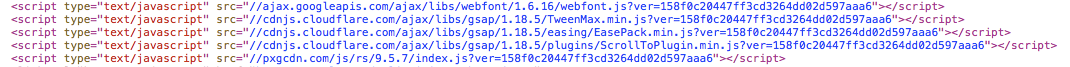
\includegraphics[width=\textwidth]{img/head.png}
  \caption{Optimalizovaná hlavička webu, zdroj: \url{lacasadegliamici.co.uk}, 26. 11. 2016}
  \label{fig:head}
\end{figure} 

\subsubsection{Fotografie}

Fotografie použité na webu byly zmenšeny na délku delší hrany 1920px (z původních 4449px) a u fotografií byly odstraněny nepotřebné meta informace. Fotografie byly dále komprimovány do datového formátu jpg. Velikost fotografie tak poklesla v průměru o 88 \% (rozdíly dle komplexnosti obrazové informace) a výsledná velikost velikost se pohybuje kolem 200kB. Z těchto fotografií byly následně vygenerovány menší obrázky pro použití na mobilních zařízeních. Obrázky byly vygenerovány s délkou delší hrany 150px, 300px a 1024px. Obrázky jsou pomocí atributu \texttt{srcset} HTML elementu \texttt{<img>} specificky načítány pro každou velikost zobrazovacího zařízení. Redukujeme tak množství přenášených dat na menších zařízeních, kde je velký obrázek zbytečný, a kde množství přenášených dat bývá zpoplatněno, nebo omezeno. Do systému webových stránek byl donahrán plugin \texttt{WP SMUSH}, který automaticky redukuje velikost nově nahrávaných obrázků - majitel restaurace tak nemusí obrázek upravovat v programu a bude mít při nahrávání nových obrázků jistotu, že budou optimalizované. 

\subsubsection{Responzivita}

Web je plně responzivní a přizpůsobuje své rozložení šířce zobrazovacího zařízení. CSS pravidla zahrnující \texttt{media-queries} jsou rozdělena do šířek:

\begin{itemize}
	\item 480px
	\item 640px
	\item 900px
	\item 1024px
	\item 1366px
\end{itemize}

Kombinací pravidel pro tyto šířky bylo docíleno toho, že stránka své rozložení přeskládává tak, aby se se stránkou dobře zacházelo na různých typech zařízení. Obsah, který je běžně rozdělen do dvou sloupců je přesklán do jednoho sloupce, aby byl text v nich obsažený lépe čitelný a obrázky lépe viditelné. Stránka je zobrazená na celou šířku zařízení, je odstraněn rámeček, který stránku ohraničuje na zařízení širším než 900px. Obrázky, které jsou na širším zařízení zobrazeny ve dvou sloupcích, jsou na menším zařízení zobrazeny v jednom sloupci a jsou vloženy pod text, který se běžně nachází vedle nich. Položky jídelního menu jsou na menším zařízení zobrazeny také v jednom sloupci.

Velké změny v zobrazení na mobilním zařízení doznalo také menu webu. To je na mobilních zařízeních reprezentováno pomocí ikony v levé horní části stránek a po kliknutí na tuto ikonu z levé hrany obrazovky vyjíždí menu přizpůsobené pro ovládání dotykem (obrázek \ref{fig:webmenu}).

 \begin{figure}
  \centering
    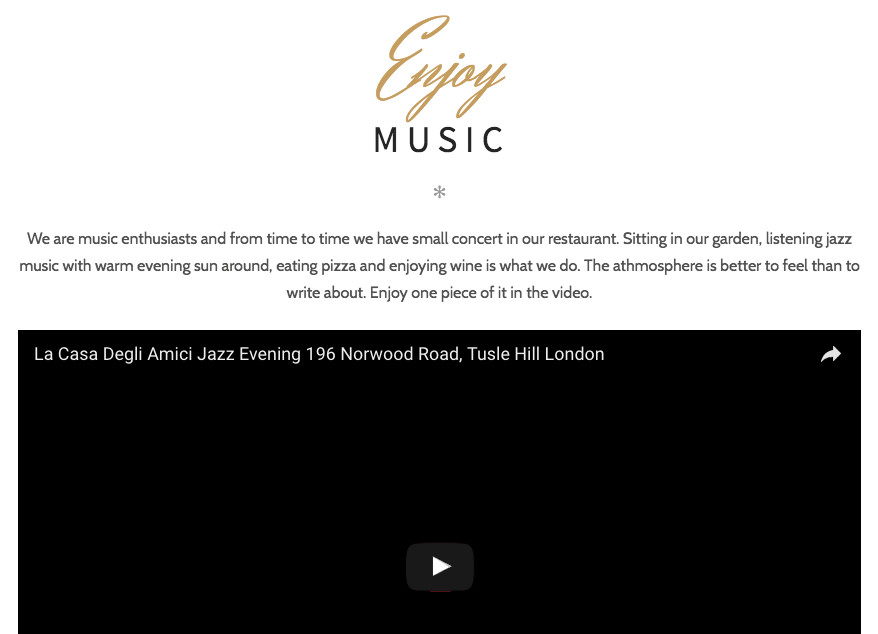
\includegraphics[width=\textwidth]{img/responsivity.png}
  \caption{Změna rozložení na mobilním zařízení (text a video jsou běžně vedle sebe), zdroj: \url{lacasadegliamici.co.uk}, 26. 11. 2016}
  \label{fig:responsivity}
\end{figure} 

 \begin{figure}
  \centering
    
\includegraphics[width=\textwidth]{img/webmenu.png}
  \caption{Menu pro mobilní zařízení, zdroj: \url{lacasadegliamici.co.uk}, 26. 11. 2016}
  \label{fig:webmenu}
\end{figure} 

Responzivita je jedním z důležitých signálů webových vyhledávačů. Posouzení kvality optimalizace bude provedeno v kapitole \ref{section:seoanalysis}.

\subsubsection{URL}
\label{section:URL}

Adresy jednotlivých stránek byly upraveny tak, aby URL adresy sémanticky popisovaly obsah stránek a uživatel z nich tak hned mohl vyčíst, co stránky obsahují. Bylo toho docíleno pomocí \texttt{.htaccess} souboru a modulu \texttt{mod\_rewrite}, který je obsažen na přiloženém CD. Struktura URL je pevná a nebude se měnit - zamezíme tak problémům s přerozdělením ohodnocení jedné stránky do více URL adres, problémům s odkazy, které nikam nesměřují a problémům s duplicitním obsahem. Nově vzniklé stránky v tomto systému dostanou unikátní adresu odvozenou od jejich názvu. 

Příklady:
\begin{itemize}
	\item \url{http://www.lacasadegliamici.co.uk/menu/starters/}
	\item \url{http://www.lacasadegliamici.co.uk/contact/}
\end{itemize}

\subsubsection{Cache}

Hosting byl nastaven tak, aby stránky, které server Apache vygeneruje, uchovával a ulehčil tak serveru práci. Dotazy na server jsou tak vyřízeny rychleji. V cache jsou mimo vygenerovaných stránek uloženy také spojené a minifikované CSS a JS soubory. Při změně původních souborů jsou soubory v cache aktualizovány. Je spuštěna také objektová cache, která uchovává často používané PHP objekty. Nastavení cache je obsaženo v \texttt{.htaccess} souboru přiloženém na CD.

Vyhodnocení technické optimalizace bude provedeno pomocí Google PageSpeed Insights v kapitole \ref{section:seoanalysis}.

\subsection{Off-page SEO}

Dle aktuálních statistik (obrázek \ref{fig:socialstats}) byla pro šíření povědomí o restauraci vybrána nejpoužívanější sociální síť Facebook, která byla provázána s populární fotografickou sociální sítí Instagram. Instagram byl také vybrán z důvodu jednoduchosti používání - majiteli restaurace stačí chytrý mobilní telefon s nainstalovanou Instragram aplikací, udělá fotografii, připíše popisný text a sdílí obsah. Na těchto sítích restaurace zveřejňuje propagační obsah, akční nabídky a soutěže. Vzhledem k tomu, že webová stránka a profily na sociálních sítích představují první online prezentaci restaurace a marketingová strategie se nejdříve musí osvědčit, nebyly zveřejněny žádné PR články, které by zvýšily množství zpětných odkazů. Pokud se současný marketingový postup osvědčí, je v plánu marketingovou strategii rozšířit. 

\begin{figure}
  \centering
    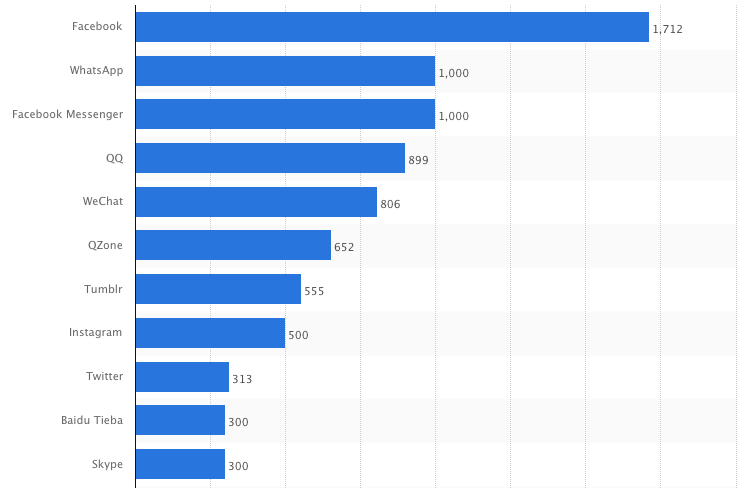
\includegraphics[width=\textwidth]{img/socialstats.png}
  \caption{Nejpoužívanější sociální sítě - počet aktivních účtů v milionech, zdroj: \url{statista.com}, 27. 11. 2016}
  \label{fig:socialstats}
\end{figure}  

\subsubsection{Facebook}

Pro restauraci byl vytvořen facebookový profil\footnote{\url{https://www.facebook.com/lacasadegliamici.co.uk/}}, který byl použit pro pozvánky na jazzové večery (obrázek \ref{fig:livejazz}) pro zveřejňování aktuálního dění v restauraci - např. galerie z proběhlých akcí (obrázek \ref{fig:jazzgalery}), pro zveřejňování nabídek (čerstvé ryby - obrázek \ref{fig:fish}, pizza za 5,95\pounds, nabídka drinků Pimm's) a soutěží o jídlo zdarma (obrázek \ref{fig:competition}). Přihlášením do soutěže uživatelé poskytli svou e-mailovou adresu, která bude v budoucnu využita pro zasílání novinek prostřednictvím služby Mailchimp\footnote{\url{http://mailchimp.com}}. Obsah byl propagován pomocí placené reklamy na Facebooku. Vyhodnocení marketingové strategie na sociálních sítích je v kapitole \ref{section:seoanalysis}.

\begin{figure}
  \centering
    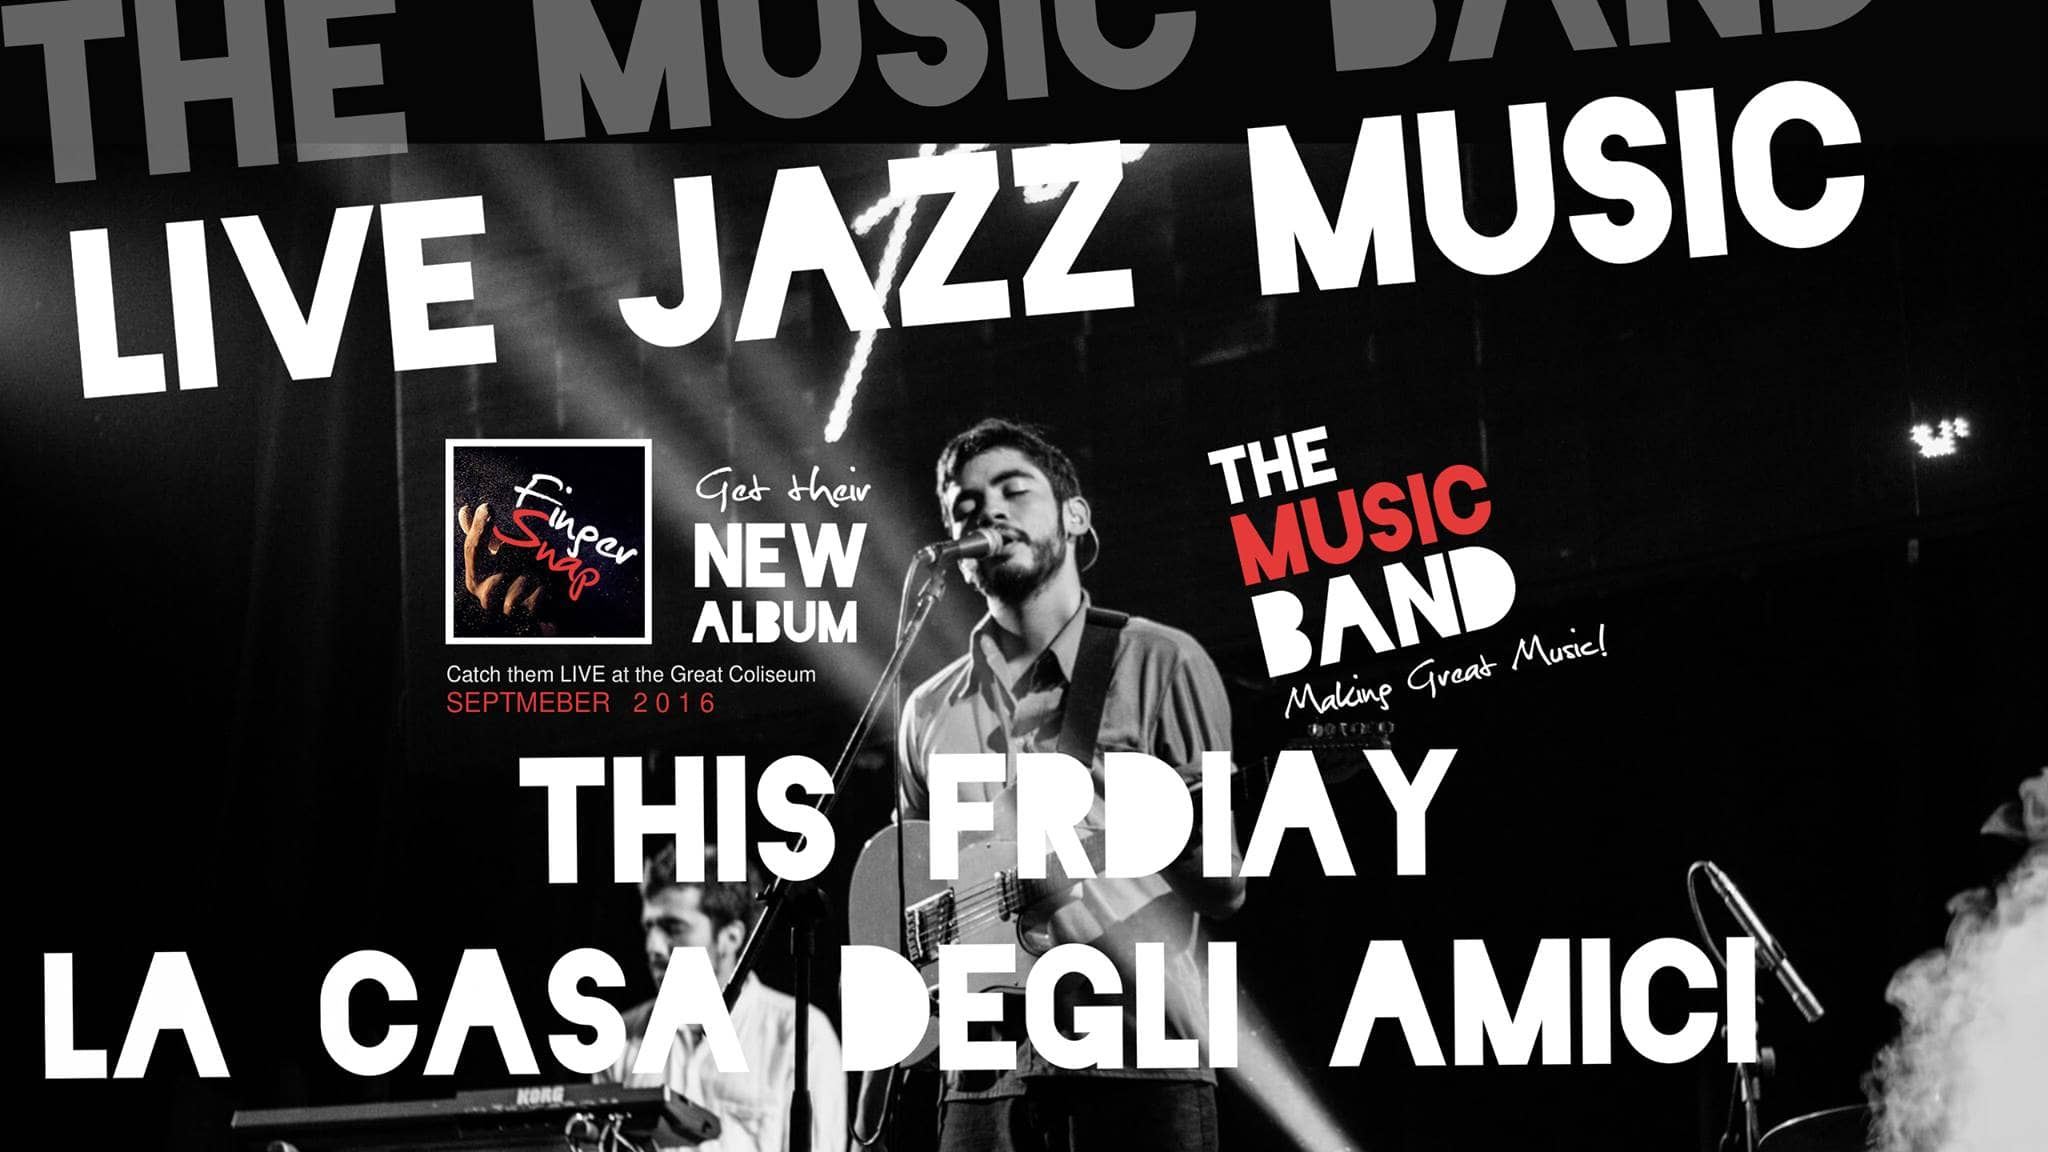
\includegraphics[width=\textwidth]{img/livejazz.jpg}
  \caption{Jedna z pozvánek na jazzový večer v restauraci La Casa Degli Amici na fb profilu}
  \label{fig:livejazz}
\end{figure} 

\begin{figure}
  \centering
    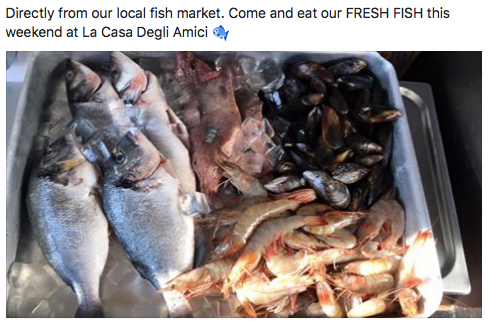
\includegraphics[width=\textwidth]{img/fish.png}
  \caption{Aktuální nabídka čerstvých ryb zveřejněná na fb profilu}
  \label{fig:fish}
\end{figure} 

\begin{figure}
  \centering
    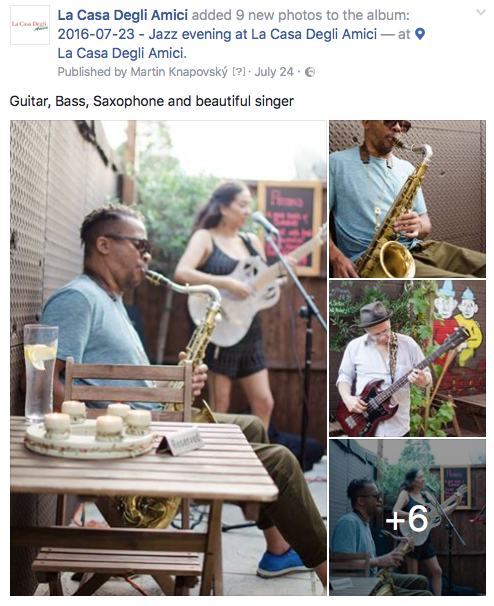
\includegraphics[width=\textwidth]{img/jazzgallery.png}
  \caption{Ukázka zveřejněné galerie na fb profilu}
  \label{fig:jazzgalery}
\end{figure} 

\begin{figure}
  \centering
    
\includegraphics[width=\textwidth]{img/competition.png}
  \caption{Soutěž o jídlo zdarma na fb profilu}
  \label{fig:competition}
\end{figure} 

\subsubsection{Instagram}

Skrze instagramový profil\footnote{\url{https://www.instagram.com/lacasadegliamici/}} byla sdílena videa a fotografie pořízené v restauraci. Obsah vložený na Instagram je automaticky vkládán i na facebookový profil restaurace. Ukázka instagramového profilu je na obrázku \ref{fig:instagram}.

\begin{figure}
  \centering
    
\includegraphics[width=\textwidth]{img/instagram.png}
  \caption{Ukázka instagramového profilu restaurace}
  \label{fig:instagram}
\end{figure} 

\subsubsection{TripAdvisor}

TripAdvisor je internetový portál věnovaný cestování a turismu. Obsahuje především recenze hotelů, restaurací, památek atd. Stránky obsahují také diskuzní fórum cestovatelů. Obsah Trip\-Advisoru je vytvářen samotnými uživateli - uživatelé sdílejí fotografie a recenzují navštívené podniky. Tripadvisor je dle statistik z roku 2016 (obrázek \ref{fig:tripstats}) nejnavštěvovanějším cestovatelským portálem, který je běžně používán i lokálně pro nalezení nových restaurací s kvalitním ohodnocením. Z tohoto důvodu jsme se na TripAdvisor zaměřili.

\begin{figure}
  \centering
    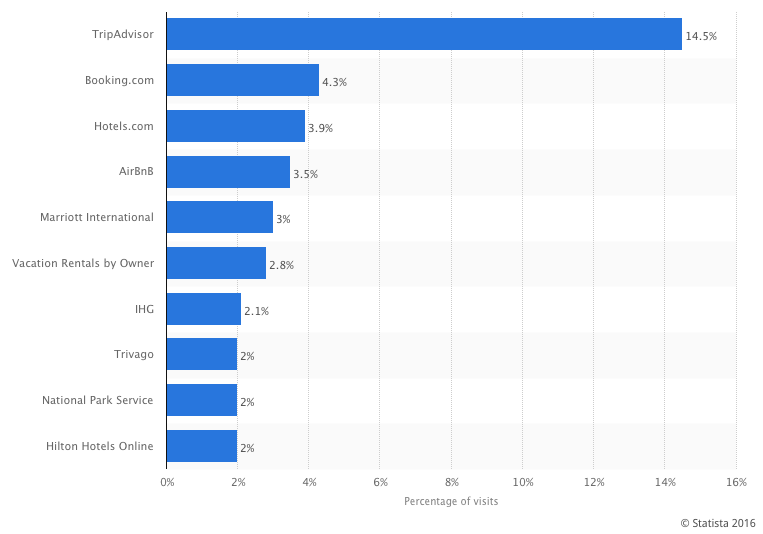
\includegraphics[width=\textwidth]{img/tripstats.png}
  \caption{TripAdvisor v porovnání s konkurencí - procento na trhu cestovatelských portálů, zdroj: \url{statista.com}}
  \label{fig:tripstats}
\end{figure} 

TripAdvisor profil se stal často používaným - pravděpodobně i proto, že na vstupní dveře restaurace byla nalepena nálepka, která podněcuje hosty k zanechání recenze. Od června 2016 do 27. 11. 2016 bylo zanecháno 49 hodnocení s průměrným ohodnocením 4,5 z 5 možných bodů. 

\begin{figure}
  \centering
    
\includegraphics[width=\textwidth]{img/triprating.png}
  \caption{Ohodnocení restaurace La Casa Degli Amici na TripAdvisor.com, zdroj: \url{tripadvisor.com}, 27. 11. 2016}
  \label{fig:tripstats}
\end{figure} 

\section{Analýza marketingové strategie}
\label{section:seoanalysis}

V této části vyhodnotíme účinnost marketingové strategie se zaměřením na vyhodnocení účinnosti SEO. Statistiky jsou získány z nástroje ahrefs, Google Webmaster Tools, Google Analytics, Facebook Insights a také od majitele restaurace. Vzhledem k vícevrstvosti modelu marketingové strategie je nejvhodnějším typem vyhodnocení změny výdělku restaurace v porovnání se stejným obdobím v minulém roce. Webová stránka byla spuštěna 1. 8. 2016, Facebookový a Instagramový profil existují od 24. 6. 2016. Vyhodnotíme nejdříve jednotlivé aspekty provedené optimalizace a poté se zaměříme na vyhodnocení celkové marketingové strategie.

\subsection{Analýza webu pomocí PageSpeed Insights}

PageSpeed Insights je nástroj, který umožňuje změřit kvalitu optimalizace webových stránek z mnoha faktorů. Tento nástroj byl představen v kapitole \ref{section:pagespeedinsights}. Vyhodnocení bylo provedeno 23. 11. 2016 s výsledkem 90/100 pro desktopová zařízení a 74/100 pro zařízení mobilní. Obrázky provedeného měření jsou kvůli svým rozměrům umístěny v příloze \ref{app:pagespeed} a jsou také umístěny na CD. 

\subsubsection{Vyhodnocení optimalizace pro desktopy}

Text se odkazuje k obrázku \ref{fig:pagespeeddesktop}. Na desktopových zařízeních web \url{www.lacasadegliamici.co.uk} splnil tato pravidla:

\begin{itemize}
	\item gzip komprese
	\item minifikace JavaScriptu
	\item minifikace CSS
	\item minifikace HTML
	\item optimalizace obrázků
	\item priorita viditelného obsahu
	\item vyhnutí se přesměrování ze vstupní stránky
	\item krátká doba odezvy 
\end{itemize}

Bylo doporučeno změnit datum vypršení platnosti dat v mezipaměti prohlížeče pro soubor \texttt{ad\_status.js}, který je načítaný skrze kód vygenerovaný na serveru Youtube. Tento soubor byl do webové stránky vložen jako HTML \texttt{<iframe>} element, který svůj obsah donačítá z umístění zadaného v jeho atributu\footnote{\url{http://www.w3schools.com/TAgs/tag_iframe.asp}} (v našem případě Youtube). Donačtený obsah může dále načítat JavaScriptové knihovny potřebné pro svou správnou funkci. Toto je právě případ souboru \texttt{ad\_status.js}, který je takto donačítán a není tedy možné změnit datum vypršení platnosti v mezipaměti prohlížeče. V druhém případě jde o stejný problém donačítání souborů - tentokrát však ze serveru \texttt{maps.google.com}. Řešením by bylo nahrát video přímo na hosting našeho webu a vynechat tak Youtube. Problém je však v tom, že se tak ochudíme o možnost efektivně sdílet obsah v síti Youtube a to je pro SEO a marketingovou strategii nevýhodné. Google Mapy by bylo také možné vynechat, avšak pokud má být web uživatelsky přívětivý, umožní jeho uživateli interaktivně pracovat s mapou přímo na našem webu, aby si mohl udělat lepší představu o poloze restaurace.

Další doporučení padlo na eliminaci blokujícího JavaScript a CSS kódu. Jak již bylo dříve uvedeno v kapitole \ref{section:minifycdn}, některé z JavaScript souborů nelze odstranit z hlavičky našich webových stránek - jedná se o soubory \texttt{jquery.js} a \texttt{jquery-migrate.min.js}. Tyto soubory jsou spojeny do jednoho souboru a ten je minifikován. Výsledný soubor je tedy při našech podmínkách optimalizovaný na nejvyšší možnou mez. Další blokující JavaScript soubory jsou knihovny, které jsou načítány z různých CDN serverů. Vzhledem k tomu, že se jedná o knihovny, které jsou často používány při stavbě dnešních webových stránek, je pravděpodobné, že je bude uživatel při načítání stránky našeho webu již mít uloženy ve vyrovnávací paměti (cache) webového prohlížeče a načte je tedy z ní a nemusí soubory načítat z CDN serveru. Ve výsledku se tedy načítání urychlí a PageSpeed Insights musíme v tomto případě brát s rezervou. 

Celkové hodnocení 90/100 je tedy maximální možné skóre, které při dodržení nejlepších postupů může náš web získat.

\subsubsection{Vyhodnocení optimalizace pro mobilní zařízení}

Zobrazení na mobilním zařízení musí splňovat stejné podmínky jako destopová zařízení, avšak ohodnocení je přísnější - na obrázku \ref{fig:pagespeedmobile} je možné vidět, že hodnocení pro mobilní zařízení upozorňuje na ty stejné problémy, které již byly popsány při analýze vyhodnocení ohodnocení pro desktopové systémy. Při ohodnocení 74/100 tak také dosahuje nejvyššího možného ohodnocení.

Hodnocení Google PageSpeed Insights se také zabývá UX designem. V případě našich stránek byla splněna všechna posuzovaná pravidla:

\begin{itemize}
	\item konfigurace viewportu (rozměrů zobrazovacího zařízení)
	\item použití čitelné velikosti písma
	\item přizpůsobení velikosti obsahu viewportu
	\item vyhnutí se nadměrnému použití pluginů
\end{itemize}

Dle hodnocení tak bylo dosaženo kvalitní responzivity a použitelnosti na desktopových i na mobilních zařízeních. Ohodnocení PageSpeed Insights je jedním z důležitých signálů, které používá vyhledávač Google k ohodnocení výsledků vyhledávání - pro SEO je tedy velmi výhodné mít technicky kvalitně optimalizované webové stránky. 

\subsection{Návštěvnost webu}

Pro hodnocení návštěvnosti webu byl použit nástroj Google Analytics, pomocí kterého byly sledovány různé faktory, které je možné vidět na obrázku \ref{fig:visitors}. Celkově bylo od spuštění webu \url{lacasadegliamici.co.uk} (1. 8. 2016) zaznamenáno do 29. 11. 2016 834 přístupů na web, ze kterého bylo shlédnuto 2301 stránek. 25 \% přístupů bylo od uživatelů, kteří již dříve web navštívili. V průměru uživatelé při jednom přístupu shlédli 2,76 stránek a setrvali na webu 2 minuty a 22 sekund.  

Návštěvnost je pro restauraci dostačující - hlavní efekt marketingové strategie uvidíme na navýšení zisku restaurace. Větší návštěvnosti lze dosáhnout aplikací off-page SEO optimalizace, která je doporučená jako další krok marketingové strategie. Jedná se o rozšíření zpětných odkazů, psaní PR a blogových článků a tvorbu mikrostránek.


\begin{figure}
  \centering
    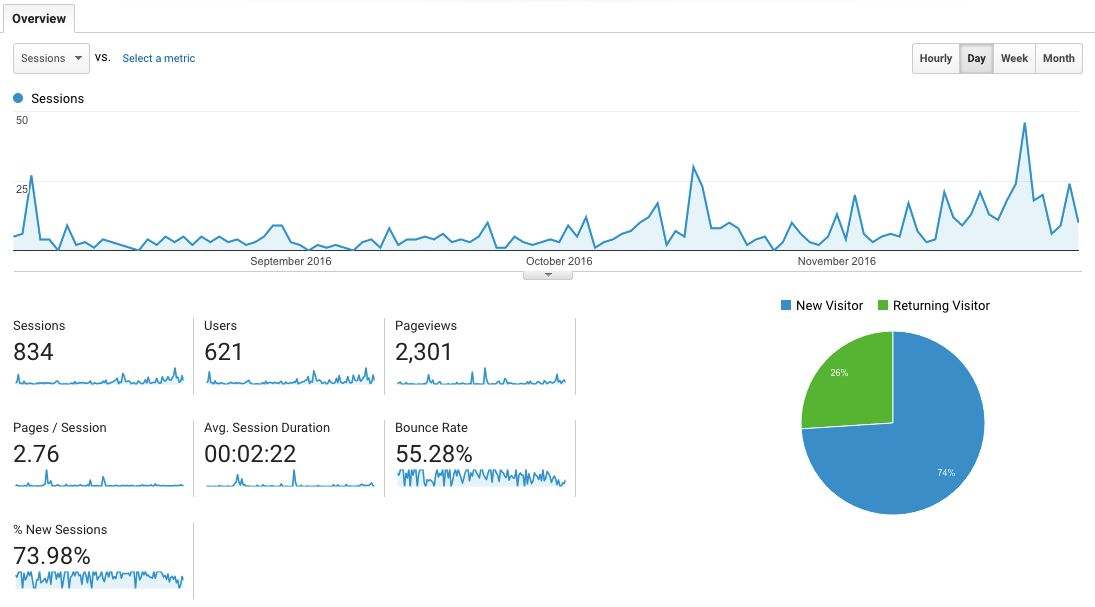
\includegraphics[width=\textwidth]{img/visitors.png}
  \caption{Analýza návštěv webu, zdroj: Google Analytics, 29. 11. 2016}
  \label{fig:visitors}
\end{figure} 

\subsection{Dostupnost a odezva serveru}

Pokud uživatel klikne na stránku, která se následně nenačte, ztrácí důvěru. Z tohoto důvodu je nutné zajistit stabilitu serveru, na kterém jsou webové stránky umístěny. Na obrázku \ref{fig:webmin} je vidět, že server byl k 29. 11. 2016 dostupný 95 dní, 16 hodin a 37 minut bez výpadku. 

\begin{figure}
  \centering
    \includegraphics[width=\textwidth]{img/webmin.png}
  \caption{Dostupnost serveru a další údaje z panelu Webmin, 29. 11. 2016}
  \label{fig:webmin}
\end{figure} 

Kvalita optimalizace serveru byla dále měřena pomocí nástroje Google Webmaster Tools. Odezva serveru postupnou optimalizací klesla až na 228ms (obrázek \ref{fig:loadingtime}). Nástroj PageSpeed Insights zhodnotil tuto délku odezvy jako vhodnou, Google doporučuje držet odezvu kolem 200ms\footnote{\url{https://developers.google.com/speed/docs/insights/Server}}.  

\begin{figure}
  \centering
    \includegraphics[width=\textwidth]{img/loadingtime.png}
  \caption{Odezva serveru, zdroj: Google Webmaster Tools, 27. 11. 2016}
  \label{fig:loadingtime}
\end{figure} 

\begin{comment}
\subsection{Indexace}

Stane se, že vyhledávací robot není schopen přečíst všechny stránky, které se na daném webu nacházejí (kapitola \ref{section:jsanalysis}). Pomocí nástroje Google Webmaster Tools bylo ověřeno, že  
\begin{figure}
  \centering
    \includegraphics[width=\textwidth]{img/site-errors.png}
  \caption{Odezva serveru, zdroj: Google Webmaster Tools, 27.11.2016}
  \label{fig:siteerrors}
\end{figure} 
\end{comment}

\subsection{Off-page}

K posílení pozice ve webových vyhledávačích je off-page optimalizace zásadní. V současném stavu je off-page optimalizace hodnocena jako nedostatečná. Pokud se aktuální strategie osvědčí, bude rozšířena o off-page SEO, které bude zahrnovat tvorbu mikrostránek na vlastních doménách, placené PR články a blogové příspěvky věnované italské kuchyni. Webové stránky restaurace jsou pro psaní takových blogových článků připraveny. I přesto, že jsme se nesoustředili na zisk odkazů, můžeme analyzovat zpětné odkazy, které vznikly samovolně. Nárůst množství odkazů je vidět na obrázku \ref{fig:refferingpages}. 

\begin{figure}
  \centering
    \includegraphics[width=\textwidth]{img/referringpages.png}
  \caption{Nárůst počtu odkazů, zdroj: ahrefs, 27. 11. 2016}
  \label{fig:refferingpages}
\end{figure} 

\begin{table}[]
\centering
\label{table:backlinks}
\begin{tabular}{lll}
Domény                   & Odkazy & Cílové stránky \\
scoop.it                 & 9     & 1              \\
youtube.com              & 5      & 1              \\
knapovsky.com            & 2      & 1              \\
findeen.co.uk            & 1      & 1              \\
irnon.com                & 1      & 1              \\
finerestaurantfinder.com & 1      & 1              \\
yellow.place             & 1      & 1             
\end{tabular}
\caption{Domény, na kterých jsou umístěny zpětné odkazy, zdroj: Google Webmaster Tools, 27.11.2016}
\end{table}

\subsection{Klíčová slova}

Pro hodnocení pokrytí klíčových slov jsme zvolily analýzu vyhledávacích řetězců, přes které se přistupovalo na webové stránky. Na obrázku \ref{fig:visitors} bylo vidět, že celkově byl web od 1. 8. do 29. 11. navštíven 834krát. Z těchto návštěv byla více než polovina (448) z vyhledávače Google. Klíčová slova, která byla použita pro vyhledávání, a ze kterých se následně přešlo na webové stránky, jsou uvedeny v tabulce \ref{table:keywordstat}   
 
\begin{table}[]
\centering
\label{table:keywordstat}
\begin{tabular}{llll}
Pořadí & Dotaz & Kliknutí & Pozice ve vyhledávači \\
1      & la casa degli amici           & 69 & 3,3 \\
2      & italian restaurant tulse hill & 44 & 1,0 \\
3      & casa degli amici              & 31 & 2,0 \\
4      & italian tulse hill            & 27 & 1,0 \\
5      & la casa degli amici london    & 24 & 2,1 \\
6      & italian restaurants near me   & 21 & 1,0 \\
7      & casa degli                    & 15 & 6,0 \\
8      & pizza tulse hill              & 11 & 10 \\
9      & la casa degli                 & 9 & 1,0 \\
10     & pizza delivery                & 9 & 1,0 \\
11     & tulse hill pizza              & 7 & 9,6 \\
12     & buffet east london            & 7 & 19 \\
13     & pizza west norwood            & 7 & 1,0 \\
14     & pizza delvery                 & 6 & 1,0
\end{tabular}
\caption{Kombinace klíčových slov, ze kterých bylo přistoupeno na web z vyhledávače Google, zdroj: Google Webmaster Tools, 29. 11. 2016}
\end{table}

Řetězec \uv{Tulse Hill}, na který jsme se soustředili, se často vyskytuje ve vyhledávání, dalším častým řetězcem je \uv{West Norwood}, což je název většího územního celku, ve kterém se nachází Tulse Hill a Herne Hill. Dle pozice ve vyhledávači lze usuzovat, že lokální pokrytí vyhledávání s řetězcem \uv{Italian restaurant} bylo úspěšné. V tabulce je na 6. místě řetězec \uv{italian restaurants near me} s pozicí 1 - toto dokazuje kvalitní lokální pokrytí Do budoucna by bylo vhodné pokrýt vyhledávání \uv{Italian Restaurant Herne Hill} a další kombinace klíčových slov obsahující lokální názvy. Kompletní statistiky jsou umístěny na CD.

\subsection{Facebook}

Restaurace na svém FB profilu získala maximální možné uživatelské hodnocení 5/5 (obrázek \ref{fig:fbreview}). Bylo zaplaceno několik kampaní, které propagovaly soutěže o jídlo a pozvánky na koncerty. Dosah příspěvků se takovouto propagací zvýšil z průměrných 500 lidí až na 8000 lidí (obr. \ref{fig:fbreach}). Hlavní publikum bylo v rozmezí 35 až 44 let (obr. \ref{fig:fbpublic}) a od 24. 6. 2016 (založení FB profilu) do 27. 11. 2016 stoupl počet kliknutí na tlačítko \uv{To se mi líbí} na 391 (obr. \ref{fig:fblikes}). Tito uživatelé dostávají na obsah, který restaurace sdílí, notifikaci a restaurace se tak lépe udržuje v povědomí těchto uživatelů.     

\begin{figure}
  \centering
    \includegraphics{img/fb-review.png}
  \caption{Uživatelské ohodnocení FB profilu restaurace, zdroj: Facebook.com, 27.11.2016}
  \label{fig:fbreview}
\end{figure}

\begin{figure}
  \centering
    \includegraphics[width=\textwidth]{img/fb-likes.png}
  \caption{Nárůst \uv{To se mi líbí} na sociální síti Facebook, zdroj: Facebook.com, 27. 11. 2016}
  \label{fig:fblikes}
\end{figure} 

\begin{figure}
  \centering
    \includegraphics[width=\textwidth]{img/fb-public.png}
  \caption{Obecenstvo FB profilu restaurace, zdroj: Facebook.com, 27. 11. 2016}
  \label{fig:fbpublic}
\end{figure} 

\begin{figure}
  \centering
    \includegraphics[width=\textwidth]{img/fb-reach.png}
  \caption{Dosah příspěvků na FB profilu restaurace, zdroj: Facebook.com, 27. 11. 2016}
  \label{fig:fbreach}
\end{figure} 

\begin{figure}
  \centering
    \includegraphics[width=\textwidth]{img/fb-views.png}
  \caption{Počet shlédnutí FB profilu restaurace, zdroj: Face\-book\-.com, 27. 11. 2016}
  \label{fig:fbviews}
\end{figure} 

\subsection{Příjmy restaurace}
\label{section:incomes}

Konečnou analýzou marketingové strategie a úspěšnosti SEO je vyhodnocení příjmů restaurace v porovnání se stejným obdobím v roce 2015. Statistiky, ze kterých byl vytvořen graf na obrázku \ref{fig:incomes} poskytl majitel restaurace Thomas Fiala. Na obrázku je možné vidět meziroční nárůst příjmů, který zvýšil příjmy přibližně o 15 - 20 \%. Od srpnu 2016 je vidět další nárůst přijmů, který přičítáme spuštění webu a propagaci na sociálních sítích. Ve 40. týdnu roku 2016 byl zaznamenána rekordní tržba 5126\pounds, která překonala tržbu z roku 2015 o 2425\pounds. 

\begin{figure}
  \centering
    \includegraphics[width=\textwidth]{img/incomes.png}
  \caption{Porovnání příjmů restaurace od června do listopadu 2015 a 2016, zdroj: La Casa Degli Amici - Thomas Fiala, 10. 11. 2016}
  \label{fig:incomes}
\end{figure} 

\section{Souhrn praktické části}

V praktické části byla ukázán návrh a implementace marketingové strategie restaurace La Casa Degli Amici. Soustředily jsme se primárně na SEO, avšak zmínili jsme také propagaci na sociálních sítích Facebook a Instagram. Webová stránky, které byly v praktické části představeny slouží pro ilustraci aplikace SEO pro marketing. Dle výše uvedených statistik lze aktuální průběh marketingové strategie a SEO označit za úspěšný - restaurace vstupuje do povědomí lidí pohybujících se v jejím okolí, o restauraci se více diskutuje (viz FB), na restauraci se sdílí více recenzí (viz TripAdvisor) a zvyšují se příjmy. Posílením marketingové strategie o rozsáhlejší off-page SEO by restaurace mohla získat ještě více.

\chapter{Závěr}

Vyhledávání se stalo běžnou součástí našich životů a změnilo způsob jakým se lidé učí, pracují, sdílejí, nakupují, zkoumají a interagují. Organizace všeho druhu - značky, charita, podnikatelé a také jednotlivci potřebují určitý druh online prezentace, která bude vyhledatelná pomocí univerzálního vyhledávače typu Google, aby se tak dostali blíže k lidem. S tím, jak se společnost stále více přesouvá do online světa, budou způsoby tvorby, publikace a distribuce stále důležitější a sofistikovanější. Práce byla stavěna hierarchicky od jednoduchého ke složitému, aby bylo možné pokrýt široké obecenstvo s minimálními nároky na vstupní znalosti a představit tak SEO jako důležitou součást marketingových strategií. V této práci jsme si ukázali, jakým způsobem fungují vyhledávače, jak lidé vyhledávají, jaký obsah je pro vyhledávače vhodný, proč je důležité tvořit kvalitní obsah, jak optimalizovat webové stránky pro vyhledávače, jakými nástroji kvalitu optimalizace analyzovat a také jak se SEO integruje do celkové marketingové strategie. V návrhové části jsme navrhli a implementovali marketingovou strategii pro londýnskou restauraci La Casa Degli Amici. Pro restauraci byl vytvořen web, profily na sociálních sítích a obsah, který byl propagován ke zvýšení povědomí o restauraci a navýšení příjmů. Výsledky strategie byly analyzovány se zaměřením na SEO a na změnu příjmů. Dle statistik v kapitole \ref{section:incomes} byl zjištěn viditelný pozitivní efekt aplikované marketingové strategie. Marketingovou strategii je doporučeno rozšířit o psaní PR článků, mikrostránek a blogových článků, které zvýší povědomí o restauraci a také počet zpětných odkazů, čímž se tak získá lepší ohodnocení ve vyhledávačích.

 Cíl práce zněl: \uv{Cílem této práce je detailně popsat aktuální způsoby optimalizace webových stránek a ukázat jejich aplikaci v širší marketingové strategii italské restaurace La Casa Degli Amici.} Troufám si tvrdit, že cíl diplomové práce byl splněn. Text je - díky jeho přístupnosti - také možné využít jako příručku pro optimalizaci vlastních webových stránek.

\newpage\thispagestyle{empty}

\appendix
\chapter{Terminologický slovník}
\label{section:dictionary}

\begin{sortedlist}

\sortitem{Markup - Sekvence znaků nebo symbolů, které jsou umístěny v textu k označení způsobu rozložení dokumentu při tisku, nebo pro popis logické struktury dokumentu.}
\sortitem{Vaporware - Označení pro produkt, který je veřejně ohlášen, avšak nikdy není prodáván, nebo zrušen.}
\sortitem{Počítačový robot - Počítačový program, který pro svého majitele opakovaně vykonává nějakou rutinní činnost - sběr dat, odesílán a zpracování požadavků, ...}
\sortitem{Hypertext - Způsob strukturování textu, který není lineární - obsahuje tzv. hypertextové odkazy, které v textu odkazují na jiný text, na který lze pomocí hyperlinku přejít.}
\sortitem{X.500 - Sada mezinárodních standardů vyvinutých Mezinárodní telekomunikační unií (ITU-T) pro adresářové služby v počítačových sítích.}
\sortitem{FTP - Protokol pro přenos souborů mezi počítači pomocí počítačové sítě. Používá protokol TCP z rodiny TCP/IP a může být používán nezávisle na použitém operačním systému.}
\sortitem{Fulltextové vyhledávání - Speciální způsob vyhledávání informací v databázích nebo v textových souborech, které jsou obvykle předem připraveny, tj. indexovány, aby bylo možno nalézt libovolné slovo (řetězec znaků) v nejkratším možném čase.}
\sortitem{USENET - Systém elektronických diskuzních skupin distribuovaný prostřednictvím internetu po celém světě. Uživatelé posílají veřejné příspěvky do skupin, které se dále dělí na vlákna.}
\sortitem{WHOIS - Databáze sloužící k evidenci údajů o majitelích internetových domén a IP adres.}
\sortitem{Klíčové slovo - V informatice je to slovo nebo identifikátor, který má specifický význam v programovacím jazyce. Význam klíčových slov se v různých jazycích liší. V knihovnictví se klíčová slova používají pro označení tématu knihy a její zařazení do katalogu, většinou výběrem slov z řízeného rejstříku. Podobně jsou na webu použitá klíčová slova při vyhledávání webových stránek.}
\sortitem{Meta informace - Metadata - Data poskytující informace o jiných datech. Například EXIF nebo ID3.}  
\sortitem{Hlavička webu - Část webové stránky, která je umístěna na jejím samotném začátku a je opakována v rámci celého webu.}
\sortitem{Webmaster - Správce internetových stránek.}
\sortitem{Outsourcing - Znamená, že firma vyčlení různé podpůrné a vedlejší činnosti a svěří je smluvně jiné společnosti čili subkontraktorovi, specializovanému na příslušnou činnost.}
\sortitem{Rekurzivní algoritmus - Rekurze je v programování situace, kdy je procedura nebo funkce volána v rámci jednoho vlákna dříve, než je dokončeno její předchozí volání.}
\sortitem{Fuzzy logika - Podobor matematické logiky odvozený od teorie fuzzy množin, v němž se logické výroky ohodnocují mírou pravdivosti. Liší se tak od klasické výrokové logiky, která používá pouze dvě logické hodnoty - pravdu a nepravdu, obvykle zapisované jako 1 a 0.}
\sortitem{Gray box - šedá skříňka - Kombinace bílé skříňky, jejíž struktura a funkce jsou transparentní a černé skříňky, která má naopak své vnitřní fungování a strukturu skrytou.}
\sortitem{HTTPS - Nadstavba síťového protokolu HTTP, která umožňuje zabezpečit spojení mezi klientem a serverem před odposloucháváním, podvržením dat a umožňuje též ověřit identitu protistrany.}
\sortitem{robots.txt - Soubor pomocí kterého můžeme povolit a zakázat indexaci webových stránek a souborů}
\sortitem{Shortcode - Řetězec, který slouží pro vkládání pluginů přímo do Wordpress stránek (bez nutnosti zásahu do PHP kódu). Shortcode je uzavřen v hranatých závorkách. }
\sortitem{Schema markup - Značky popisující obsah webových stránek pomocí značek uveřejněných na \url{schema.org}. Slouží k předání informace o významu obsahu pro vyhledávače, které jsou schopny tuto informaci zpracovat. }
\sortitem{ID3 tag - Kontejner pro metadata, který byl primárně vyvinut pro počítačový hudební formát MP3, lze jej však nelézt i jinde.}
\sortitem{Layout - Grafické rozvržení tiskové nebo elektronické stránky, případně i jiné plochy.}
\sortitem{Linkbuilding - Práce za účelem získání zpětného odkazu - jedná se například o psací do diskusí/fór a sociálních sítí za účelem získání zpětných odkazů (primární účel: zpětný odkaz, sekundární: noví návštěvníci)}
\sortitem{SEO – Search Engine Optimization – Optimalizace pro vyhledávače.}
\sortitem{SEM – Search Engine Marketing – Marketing ve vyhledávačích (Sklik, Adwords).}
\sortitem{PPC – Pay per Click – Platba za proklik. PPA – Pay per Action – Platba za akci (konverzi).}
\sortitem{CPM – Cost per Mile – Cena za 1000 zobrazení.}
\sortitem{CTR – Click–through rate – Míra prokliku, vyjadřuje poměr kliknutí k počtu zobrazení.}
\sortitem{SERP – Search engine results page – Stránka s výsledky vyhledávání.}
\sortitem{Adwords – PPC reklamní systém od společnosti Google.}
\sortitem{URL – Uniform Resource Locator – Internetová adresa webové stránky.}
\sortitem{Tagy (elementy) – Značky, které se používají při psaní (x)html kódu.}
\sortitem{Sémantika – Stylistická pravidla pro správné využití (x)html elementů.}
\sortitem{Zpětné odkazy – Back links – Zpětný odkaz je odkaz, který vede na web z jiného webu. Množství a kvalita zpětných odkazů ovlivňuje off-page faktory webu. Odkazy mají největší vliv na hodnotu ranku vyhledávačů.}
\sortitem{ROI – Return on Investment – Návratnost investice. Jedná se o poměr zisku a investované částky.}
\sortitem{Metadata – Informace uložené v hlavičce webu.}
\sortitem{Copywriting – Psaní textu pro web.}
\sortitem{Keyword – Klíčové slovo.}
\sortitem{Sitemapa webu – Jedná se o hierarchicky seřazený seznam všech stránek webu. Pomáhá vyhledávači najít stránky, které jsou umístěné hluboko ve stromové struktuře webu.}
\sortitem{TLD – Top Level Domain – Domena první úrovně (např .cz).}
\sortitem{CSS – Cascading Style Sheets – Kaskádové styly.}
\sortitem{Black-hat SEO – Nepovolené praktiky SEO, které vyhledávače postihují.}
\sortitem{Keyword stuffing – Nesmyslné nadměrné používání klíčových slov v textu webu. Patří mezi nepovolené praktiky SEO a vyhledávače mohou takovéto weby penalizovat.}
\sortitem{Long Tail – Dlouhý ocas – Často vyhledávaná slova tvoří jen malou část z celkových dotazů ve vyhledávači. Většina vyhledávaných frází je hledána třeba jen jednou nebo málokdy. Většinu dotazů ve vyhledávači tvoří právě málo vyhledávané fráze.}
\sortitem{Navigační dotaz – Navigational query – Hledání webu pomocí vyhledávání doménového jména ve vyhledávači.}
\sortitem{UIP – Počet návštěvníků s unikátní IP adresou za určité období.}
\sortitem{Visit – Návštěva – Většina počítadel započítává jednu návštěvu jednoho návštěvníka max. jednou za 30 minut. Impression – Imprese – Udává počet zobrazení (např. počet zobrazení reklamního banneru).}
\sortitem{Validita – Aby byl web validní, musí dodržovat předepsané standarty (např. W3C).}
\sortitem{W3C – World Wide Web Consortium – Mezinárodní konsorcium, které vyvíjí webové standarty.}
\sortitem{Katalog – Seznam webů uspořádaných do kategorií.}
\sortitem{Description – Meta tag description by měl obsahovat stručný popis dané stránky webu.}
\sortitem{Konverze – Provedení určité akce na webu – např. nakoupení zboží, přihlášení se k odběru novinek apod.}
\sortitem{Subdoména – Doména 3., nebo nižšího řádu.}
\sortitem{Traffic – Návštěvnost.}
\sortitem{Volná shoda – Veškeré dotazy ve vyhledávačích, které obsahují dané klíčové slovo.}
\sortitem{Přesná shoda – Patří sem veškeré dotazy ve vyhledávačích, které jsou hledány pomocí přesného znění hledané fráze.}
\sortitem{Slider - Obrázková galerie, u které lze mezi obrázky přecházet pomocí šipek na obrazovce nebo na klávesnici}
\sortitem{PHP Timeout} - Doba, po kterou může být provádět PHP skript

\end{sortedlist}

\chapter{Aktualizace Google Algoritmů}
\label{app:GoogleUpdates}
\begin{itemize}
\item \textbf{1996} - Vznik algoritmu PageRank - hodnocení relevatnosti webových stránek na základě počtu a kvality odkazů, které na ně odkazují
\item \textbf{02/2003} - Boston - Aktualizace indexu, která způsobila fluktuaci pořadí výsledků.
\item \textbf{04/2003} - Cassandra - Google začal penalizovat skryté texty, odkazy a tzv. Link-farmy, které byly používány pro získání lepšího ohodnocení.
\item \textbf{05/2003} - Dominic - Změna ve způsobu analýzy zpětných odkazů.
\item \textbf{06/2003} - Esmeralda - Příprava na přechod od měsíčních aktualizací indexu na denní aktualizace.
\item \textbf{07/2003} - Fritz - Namísto měsíčního indexování začal Google indexovat na denní bázi, což přinášelo aktuálnější výsledky a hodnocení. 
\item \textbf{09/2003} - Google vytvořil doplňkový index dokumentů, které dle PageRank algoritmu nebyly důležité. Zvýšil se tak celkový počet indexovaných dokumentů bez ztráty kvality výsledků vyhledávání.
\item \textbf{11/2003} - Florida - Velká změna, která zneplatnila některé staré SEO techniky jako např. Keyword stuffing. Mnoho bussinessů končí, Google lépe rozumí kontextu.
\item \textbf{01/2004} - Austin - Pokračování penalizace SEO technik - penalizace META stuffingu a neviditelného textu.
\item \textbf{02/2004} - Brandy - Velký nárůst počtu indexovaných dokumentů. Implementace LSI (Latent Semantic Indexing), lepší porozumění synonym a kontextu. Lepší analýza klíčových slov.
\item \textbf{01/2005} - NoFollow Update - Google implementuje ochranu před spamem, který se uveřejňoval na blozích a fórech ve formě spamových odkazů, které zvyšovaly PageRank cílového dokumentu.
\item \textbf{02/2005} - Allegra - Vylepšení LSI
\item \textbf{05/2005} - Bourbon - Změna v indexaci duplicitního obsahu. 
\item \textbf{06/2005} - XML Sitemaps - Google umožnil odeslání XML mapy webu skrze webmaster tools a zlepšit tak schopnost indexovat web.
\item \textbf{06/2005} - Počátek sběru dat z uživatelského vyhledávání pro personalizaci výsledků. 
\item \textbf{10/2005} - Provázání výsledků s Google Maps a poskytnutí lepších lokálních výsledků.
\item \textbf{10/2005} - Jagger - Aktualizace, která se čistě soustředí na boj proti spamu. Penalizace odkazových farem a placených odkazů. 
\item \textbf{11/2005} - Big Daddy - Nový procházecí a indexovací systém. URL canonicalization a přesměrování. Odstranění stránek nízké kvality. 
\item \textbf{05/2007} - Universal Search - Do výsledků vyhledávání byly přidány novinky, videa, obrázky a další obsah, který byl relevantní s vyhledávaným řetězcem.
\item \textbf{02/2009} - Podpora Canonical Tagu, který umoňuje vyhledávači sdělit, kde se v případě duplicitního obsahu nachází obsah původní. 
\item \textbf{11/2009} - Real-Time Search - Do výsledků vyhledávání byly přidány výsledky z Twitter Feedu, Google News a později také ze sociálních sítí. 
\item \textbf{04/2010} - Přidání lokální placené reklamy do výsledků vyhledávání.
\item \textbf{06/2010} - Caffeine - Zmeny tzv. Caffeine algorimu. Zrychlení vyhledávání a o 50 \% čerstvější index. 
\item \textbf{08/2010} - Google Instant Update - Zobrazování výsledků už ve chvíli, kdy uživatel zadával řetězec s dotazem.
\item \textbf{10/2010} - Negative reviews - Penalizace dokumentů, které získávaly vysokou pozici díky množství negativních referencí. viz DecorMyEyes 
\item \textbf{12/2010} - Social Signals - Mezi signály se zařadil Twitter a Facebook
\item \textbf{01/2011} - Overstock penalty - Přímý útok Googlu na spammery. Webmasteři overstock.com využívaly značného množství black-hat SEO technik.
\item \textbf{03/2011} - Farmer a Panda - Jedna z nejdůležitějších aktualizací, která postihla přibližně 12 \% uživatelských dotazů. Aktualizace se opět zaměřuje na spam a penalizuje automaticky generovaný obsah a weby zneužívající AdSense.
\item \textbf{04/2011} - Panda 2 - Google začíná sbírat data o webech, které uživatelé zablokovali a chápe tyto weby jako nevhodné.
\item \textbf{06/2011} - Panda 2.2 - Aktualizace se zaměřuje na weby, které duplikují obsah a penalizuje je.
\item \textbf{11/2011} - Freshness update - Tato aktualizace ovlivnila 35 \% dotazů. Google se zaměřil na prioritizaci obsahu, který je časově novější.
\item \textbf{01/2012} - Google ohlásil radikální změnu v personalizaci výsledků, agresivně do výsledků vkládá Google+ data. Přidává také tlačítko na vypnutí personalizace.
\item \textbf{04/2012} - Penguin - Další update, který bojuje proti spamu - keyword stuffing, ovlivnil 3,1 \% anglických dotazů.
\item \textbf{05/2012} - Knowledge Graph - Google spustil knowledge graph, který přidává dodatečné informace o objektech
\item \textbf{08/2012} - Google začíná penalizovat weby, které obdržely DMCA požadavky na stažení obsahu. 
\item \textbf{09/2012} - EMD (Exact-Match Domain) aktualizace 
\item \textbf{09/2012} - Panda aktualizace \#20
\item \textbf{10/2012} - Balík 65 aktualizací obsahující aktualizaci Knowledge Graph a změnu ohodnocení kvality stránek
\item \textbf{10/2012} - Penguin aktualizace \#3
\item \textbf{12/2012} - Knowledge Graph pro španělštinu, francouzštinu, němčinu, portugalštinu, japonštinu, ruštinu a italštinu. Rozšíření možností Knowledge Graphu
\item \textbf{12/2012} - Panda aktualizace \#23 - ovlivnění 1,3 \% výsledků
\item \textbf{03/2013} - Poslední Panda aktualizace před začleněním tohoto algoritmu do jádra vyhledávacích algoritmů
\item \textbf{05/2013} - Phantom aktualizace (bez podrobností o změnách)
\item \textbf{05/2013} - Domain Crowding (bez podrobností o změnách)
\item \textbf{05/2013} - Penguin 2.0 (bez podrobností o změnách)
\item \textbf{06/2013} - Panda Dance (bez podrobností o změnách)
\item \textbf{06/2013} - Payday Loan aktualizace - zaměřuje se na potírání spamu propagující půjčky a porno stránky
\item \textbf{07/2013} - Aktualizace Knowledge Graphu - rozšíření výsledků s Knowledge Graphem o 50,4 \%
\item \textbf{08/2013} - Aktualizace zvýhodňující čerstvý obsah, který se hloubkově zabývá specifickým tématem
\item \textbf{08/2013} - Hummingbird aktualizace - zlepšení sémantické analýzy obsahu
\item \textbf{10/2013} - Penguin 2.1 (bez podrobností o změnách)
\item \textbf{12/2013} - Authorship Shake-up\footnote{\url{http://www.hivedigital.com/2013/12/19/authorshippocalypse-google-authorship-penguin-finally-appeared/}} aktualizace 
\item \textbf{02/2014} - Page Layout aktualizace \#3 - Page Layout penalizuje stránky s vetším množstvím reklamy
\item \textbf{05/2014} - Payday Loan 2.0 aktualizace - redukce spamu
\item \textbf{05/2014} - Panda 4.0 - Ovlivněno 7,5 \% vyhledávání v anglickém jazyce
\item \textbf{06/2014} - Payday Loan 3.0 - boj se spamem
\item \textbf{06/2014} - Odstranění fotografií autorů
\item \textbf{07/2014} - Pigeon - změna ohodnocení lokálních výsledků
\item \textbf{08/2014} - HTTPS/SSL aktualizace - Google preferuje načítání webových stránek prostřednictvím zabezpečených protokolů
\item \textbf{09/2014} - Panda 4.1 - změna 3 \- 5 \% výsledků
\item \textbf{10/2014} - Změna rozložení bloku výsledků novinek
\item \textbf{10/2014} - Penguin 3.0 - změna <1 \% výsledků
\item \textbf{10/2014} - Pirate 2.0 - Boj s porušováním autorských práv
\item \textbf{12/2014} - Rozšíření Pigeon z 07/2014 - rozšíření na UK, Kanadu a Austrálii
\item \textbf{04/2015} - Mobilegeddon - upřednostnění respozivních webů
\item \textbf{07/2015} - Panda 4.2 (bez podrobností o změnách)
\item \textbf{10/2015} - RankBrain - Začlenění strojového učení do ohodnocování výsledků
\item \textbf{02/2016} - Aktualizace systému AdWords
\item \textbf{05/2016} - Mobile-friendly 2 aktualizace - upřednostnění responzivních webů
\item \textbf{09/2016} - Penguin 4.0 - Penguin algoritmus začleněn do jádra vyhledávače
\end{itemize}


\chapter{PageSpeed měření ze dne 23. 11. 2016}
\label{app:pagespeed}

\begin{figure}
  \centering
    \includegraphics[width=\textwidth]{img/pagespeed-desktop.png}
  \caption{PageSpeed Insights ohodnocení desktopové verze webu, zdroj: \url{https://developers.google.com/speed/pagespeed/insights}}
  \label{fig:pagespeeddesktop}
\end{figure} 

\begin{figure}
  \centering
    \includegraphics[width=\textwidth]{img/pagespeed-mobile.png}
  \caption{PageSpeed Insights ohodnocení mobilní verze webu, zdroj: \url{https://developers.google.com/speed/pagespeed/insights}}
  \label{fig:pagespeedmobile}
\end{figure} 

\chapter{Seznam příloh na CD}

\section{Adresářová struktura}
\begin{forest}
  for tree={
    font=\ttfamily,
    grow'=0,
    child anchor=west,
    parent anchor=south,
    anchor=west,
    calign=first,
    inner xsep=7pt,
    edge path={
      \noexpand\path [draw, \forestoption{edge}]
      (!u.south west) +(7.5pt,0) |- (.child anchor) pic {folder} \forestoption{edge label};
    },
    before typesetting nodes={
      if n=1
        {insert before={[,phantom]}}
        {}
    },
    fit=band,
    before computing xy={l=15pt},
  }  
[CD
  [Dokumenty
  ]
  [Fotografie
  ]
  [Google
  ]
  [Server
  ]
  [Video
  ]
  [Web
  ]
]
\end{forest}

\section{Popis}
V adresáři \texttt{Dokumenty} lze nalézt zdrojový \LaTeX~kód této diplomové práce. V adresáři \texttt{Fo\-to\-gra\-fie} se nacházejí fotografie propagující restauraci La Casa Degli Amici. Tyto fotografie byly použity při tvorbě webu. Adresář \texttt{Google} obsahuje v souboru \texttt{Mega SERP}\footnote{zdroj: \url{https://moz.com/blog/mega-serp-a-visual-guide-to-google}} přehled všech možných prvků, které se mohou objevit ve výsledcích vyhledávání Google. Dále jsou zde obsaženy statistiky z Google Analytics - soubor \texttt{Search Analytics.csv}. V adresáři \texttt{Server} se nacházejí soubory \texttt{htaccess} (viz kapitola \ref{section:URL}), \texttt{lacasadegliamici.co.uk.conf} (nastavení virtuálního serveru Apache), snímky obrazovky potvrzující ohodnocení nástrojem Google PageSpeed Insights z 23. 11. 2016, soubor \texttt{robots.txt} určující chování vyhledávacích robotů a soubor \texttt{phpinfo()}, ve kterém je možné nalézt kompletní nastavení použitého hostingu. Adresář \texttt{Video} obsahuje videa použitá pro propagaci restaurace na sítích Youtube a Instagram a adresář \texttt{Web} obsahuje kompletní webové stránky včetně databáze. Pro přístup do administrace je možné použít uživatelské jméno \texttt{knam00} a heslo \texttt{thesis2016}.


\vspace{\fill}

\newpage\addcontentsline{toc}{chapter}{Literatura} 
\label{section:bib}
\begin{thebibliography}{1}
\bibitem{usageresearch2}
ZHU, C. \textit{Proceedings: the Third International Conference on Multimedia Information Networking and Security}. 1. Los Alamitos: IEEE Computer Society, 2011, s.~225-228. ISBN 978-1-4577-1795-6.

\bibitem{usageresearch}
PURCELL, KRISTEN. Search and email still top the list of most popular online activities. In: \textit{PewResearchCenter} [online]. Washington DC, 2011 [cit. 2016-11-03]. Dostupné z: \url{http://www.pewinternet.org/2011/08/09/search-and-email-still-top-the-list-of-most-popular-online-activities/}

\bibitem{ataleoftwostudies}
A TALE OF TWO STUDIES: Establishing Google \& Bing Click-Through Rates. In: \textit{Relevance.com} [online]. Indianapolis: Relevance.com, 2015 [cit. 2016-11-03]. Dostupné z: \url{http://digital.relevance.com/hubfs/Rebranded\_Case\_Studies/WhitePaper\_ATaleofTwoStudies\_RELEVANCE\_2015.pdf?}t=1478195168961

\bibitem{dreammachines}
NELSON, Theodor. \textit{Computer lib: you can and must understand computers now}. \uv{First edition}--cover. South Bend?: Nelson, 1975. ISBN 08-934-7002-3.

\bibitem{literarymachines}
NELSON, Theodor. \textit{Literary machines: the report on, and of, project Xanadu concerning word processing, electronic publishing, hypertext, thinkertoys, tomorrow's intellectual revolution, and certain other topics including knowledge, education and freedom}. Sausalito, CA: Mindful Press, 1992. ISBN 08-934-7062-7.

\bibitem{aswemaythink}
BUSH, Vannervar. As We May Think. \textit{The Atlantic}. 1945.

\bibitem{Jansen2008}
JANSEN, Bernard J., Danielle L. BOOTH a Amanda SPINK. Determining the informational, navigational, and transactional intent of Web queries. \textit{Information Processing}. 2008, \textbf{44}(3), 1251-1266. DOI: 10.1016/j.ipm.2007.07.015. ISSN 03064573. Dostupné také z: \url{http://linkinghub.elsevier.com/retrieve/pii/S030645730700163X}

\bibitem{Enge2015}
ENGE, Eric., Stephan. SPENCER, Rand. FISHKIN, Jessie C. STRICCHIOLA a John. BATTELLE. \textit{The Art of Seo / Eric Enge, Stephan Spencer, Rand Fishkin and Jessie C. Stricchiola ; foreword by John Battelle}. 3rd Edition. Sebastopol, Calif.: O'reilly, 2015. ISBN 05-965-1886-2.

\bibitem{Hamel2008}
HAMEL, Stéphane. Web Analytics vendors market shares. In: \textit{S.Hamel’s blog} [online]. 2008 [cit. 2016-11-04]. Dostupné z: \url{http://blog.immeria.net/2008/01/web-analytics-vendors-market-shares.html}

\bibitem{Mukherjee2003}
MUKHERJEE, Shibnath. \textit{A Probabilistic Model for Optimal Searching of the Deep Web}. 2003. DOI: 10.1.1.12.4308.

\bibitem{Hussien2014}
HUSSIEN, A.S. Factors Affect Search Engine Optimization. \textit{IJCSNS International Journal of Computer Science and Network Security}. 2014, 2014(9), 28-33.

\bibitem{Battelle2005}
BATTELLE, John. \textit{The search: how Google and its rivals rewrote the rules of business and transformed our culture}. New York: Portfolio, 2005. ISBN 18-578-8361-6.

\bibitem{Fishkin2015}
FISHKIN, Rand a Moz Staff. Beginners Guide to SEO. \textit{Moz.com} [online]. 2015: Moz.com, 2015 [cit. 2016-11-05]. Dostupné z: \url{https://moz.com/beginners-guide-to-seo}

\bibitem{Huang2014}
HUANG, Wei Zhong. Research on Web Search Engine Optimization and its Application. \textit{Applied Mechanics and Materials}. 2014, \textbf{687-691}, 1908-1911. DOI: 10.4028/www.scientific.net/AMM.687-691.1908. ISSN 1662-7482. Dostupné také z: \url{http://www.scientific.net/AMM.687-691.1908}

\bibitem{Gunjan2012}
GUNJAN, Vinit Kumar, Pooja, Monica KUMARI a Dr Amit KUMAR. Search engine optimization with Google. \textit{IJCSI International Journal of Computer Science Issues}. Greater Noida, India: Department of computer science and engineering, School of engineering \& technology, Sharda University, 2012, \textbf{2012}(9), 206-214. ISSN 1694-0814.

\bibitem{Aull2014}
AULL, Jake. \textit{WordPress SEO success: search engine optimization for your WordPress Website or blog}. Indianapolis: Que, 2014. ISBN 07-897-5288-3.

\bibitem{Kubicek2008}
KUBÍČEK, Michal. \textit{Velký průvodce SEO: jak dosáhnout nejlepších pozic ve vyhledávačích}. Brno: Computer Press, 2008. ISBN 978-80-251-2195-5.

\bibitem{Collins2015}
COLLINS, Tyler. \textit{Google Ranking Factors: SEO Is Not Dead} [online]. 2015: The Huffington Post Blog, 2015 [cit. 2016-11-08]. Dostupné z: \url{http://www.huffingtonpost.com/tyler-collins/google-ranking-factors-se_b_6823786.html}

\bibitem{Dean2016}
DEAN, Brian. We Analyzed 1 Million Google Search Results. Here’s What We Learned About SEO. In: \textit{Backlinko} [online]. 2016 [cit. 2016-11-08]. Dostupné z: \url{http://backlinko.com/search-engine-ranking}

\bibitem{Martin2016}
MARTIN, James. Top 6 SEO Ranking Factors of 2016. \textit{CIO.com} [online]. 2016 [cit. 2016-11-08]. Dostupné z: \url{http://www.cio.com/article/3104104/search/top-6-seo-ranking-factors-of-2016.html}

\bibitem{WikiPageRank}
PageRank. In: \textit{Wikipedia: the free encyclopedia} [online]. San Francisco (CA): Wikimedia Foundation, 2001- [cit. 2016-11-11]. Dostupné z: \url{https://en.wikipedia.org/wiki/PageRank}

\bibitem{Zoltan2006}
ZOLTÁN, Gyöngyi, BERKHIN Pavel, Garcia-Molina HECTOR a Pedersen JAN. Link spam detection based on mass estimation. In: \textit{Proceedings of the 32nd International Conference on Very Large Data Bases (VLDB '06, Seoul, Korea)}. 2006, s.~439-450.

\bibitem{PageRankPatent}
PAGE, Lawrence. \textit{Method for node ranking in a linked database}. USA. US7058628. Zapsáno 2.6.2001.

\bibitem{Page1998}
PAGE, Lawrence a Sergey BRIN. The anatomy of a large-scale hypertextual Web search engine. \textit{Computer Networks and ISDN Systems}. 1998, \textbf{30}(1-7), 107-117. DOI: 10.1016/S0169-7552(98)00110-X.

\bibitem{Page1998_2}
PAGE, Lawrence, Sergey BRIN, Rajeev MOTWANI a Terry WINOGRAD. \textit{The PageRank citation ranking: Bringing order to the Web} [online]. 1998, \textbf{1998} [cit. 2016-11-11]. Dostupné z: \url{http://ilpubs.stanford.edu:8090/422/1/1999-66.pdf}

\bibitem{Granka2010}
GRANKA, Laura A. The Politics of Search: A Decade Retrospective. \textit{The Information Society}. 2010, \textbf{26}(5), 364-374. DOI: 10.1080/01972243.2010.511560. ISSN 0197-2243. Dostupné také z: \url{http://www.tandfonline.com/doi/abs/10.1080/01972243.2010.511560}

\bibitem{KonradBecker2009}
BECKER, Konrad \textit{Deep search: the politics of search beyond Google}. Innsbruck: Studien Verlag, 2009. ISBN 978-370-6547-956.

\bibitem{Doctorow2001}
DOCTOROW, Cory. Metacrap: Putting the torch to seven straw-men of the meta-utopia. \textit{ELearningGuru} [online]. 2001 [cit. 2016-11-14]. Dostupné z: \url{http://www.well.com/~doctorow/metacrap.htm}

\bibitem{Flynn1996}
FLYNN, Larry. \textit{Desperately Seeking Surfers} [online]. New York Times, 1996 [cit. 2016-11-14]. Dostupné z: \url{http://www.nytimes.com/1996/11/11/business/desperately-seeking-surfers.html}

\bibitem{Gyongyi2005}
GYONGYI, Zoltan a Hector GARCIA-MOLINA. Link Spam Alliances. \textit{Proceedings of the 31st VLDB Conference} [online]. Trondheim, Norsko, 2005 [cit. 2016-11-14]. Dostupné z: \url{http://infolab.stanford.edu/~zoltan/publications/gyongyi2005link.pdf}

\bibitem{Cutts2009}
CUTTS, Matt. \textit{PageRank Sculpting} [online]. 2009 [cit. 2016-11-14]. Dostupné z: \url{https://www.mattcutts.com/blog/pagerank-sculpting/}

\bibitem{Komarek2009}
KOMÁREK, Miroslav. \textit{SEO optimalizace webových stránek} [online]. Praha, 2009 [cit. 2016-11-16]. Diplomová práce. Vysoká škola ekonomická, Praha. dostupné z: \url{http://theses.cz/id/ssniks/}.

\bibitem{Grimmich}
GRIMMICH, Š. \textit{SEO - Zpětné odkazy} [online]. 2007 [cit. 2016-10-28]. dostupné z: \url{http://www.tvorba-webu.cz/seo/zpetne_odkazy.php}

\end{thebibliography}

\end{document}
